% !TeX root = ../车云协同液罐车防侧翻行驶规划与控制研究.tex

\chapter{车端防侧翻轨迹跟踪控制与模型试验}
\label{chap04_antirollover_control}
根据第\ref{chap03_vehicle_cloud_collaborate}章关于车云协同液罐车防侧翻体系架构的分析，车端需要具备状态性风险的实时识别与干预能力，并通过失效冗余防止风险进一步演变为事故。其核心在于两点：一是车辆实时稳定性干预，二是失效条件下的应急处置保障。本章聚焦于车端防侧翻轨迹跟踪控制。首先，建立车液耦合动力学模型并介绍横纵耦合液体晃动建模方法；其次，构建面向防侧翻轨迹跟踪控制的优化问题；最后，搭建车液耦合联合仿真平台，并通过缩比例模型车试验验证车端稳定性干预能力。


\section{横纵向耦合液体晃动建模}
    \label{sec:liquid_sloshing}
    % TODO:与引言部分动力学模型相呼应
    
    横纵向耦合液体晃动建模是进行防侧翻控制的第一步。本文采用机械等效模型谱系中的低阶等效力/力矩表征方法，其关键在于使模型输入输出特性与实际液体晃动对罐体的作用一致，而不是替代CFD对完整流场的重构。如图~\ref{fig:sloshing_modeling}所示，以往研究中普遍关注侧倾平面内的二维液体流动，并将其建模为各种类型的摆（单摆\cite{zhaoweiqiang2018equivalent}、椭圆摆\cite{salem2000rollover}、多质量椭圆摆\cite{yangxiujian2018multimass}等），在二维平面内能有效反映液体晃动带来的罐液耦合力特性。
    \begin{figure}
    \centering
    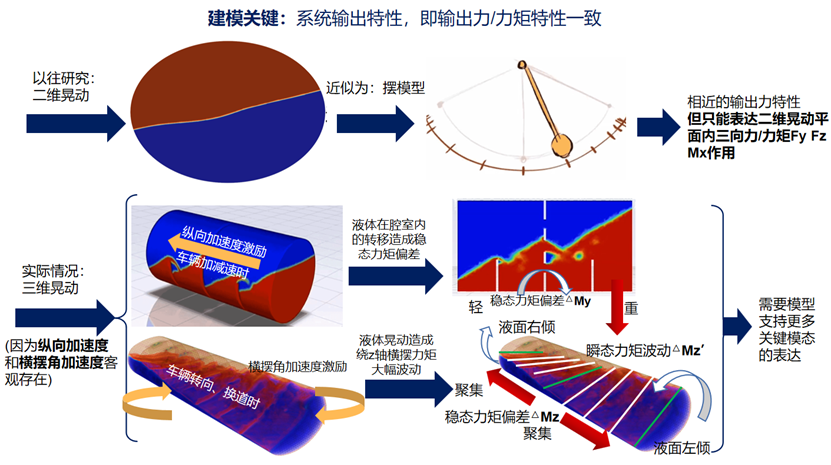
\includegraphics[width=1.0\linewidth]{fig/chap4/sloshing_modeling.png}
    \caption{多模态罐内液体非线性模型建立分析}
    \label{fig:sloshing_modeling}
    \end{figure}

    二维晃动模型对于垂向力、侧向力以及侧倾力矩三个指标已能达到较高建模精度\cite{Komasa2023observing}，但其高精度通常依赖二维晃动假设，难以完整反映实际罐内液体运动。真实行驶过程中，纵向加速度和横摆角加速度客观存在，液体晃动具有明显三维特征。除横纵向流动耦合外，液体在腔室间转移会造成稳态俯仰力矩偏差；车辆转向时，横摆角加速度还会激励罐体两侧方向相反的液体晃动，并引起横摆力矩波动。这些动态均会影响行驶稳定性，但难以由传统二维模型充分表达。

    同时，根据第~\ref{subsubsec:resource_analysis}节资源分析的结果，云端需构建高效高保真的车液耦合仿真平台，以支撑算法仿真测试。该平台依赖高保真液罐车动力学仿真模型、典型仿真工况和仿真器，而罐液耦合模型是高保真快速仿真的基础。因此，需要建立一种既能表达更多关键模态，又能满足快速计算需求的机械等效模型。

    \subsection{滑动伸缩天平模型}
        \label{sub:sliding_telescopic_libra_model}
        \subsubsection{曲面滑动质点建模与计算}
            由于车辆在纵向上按规定至少每间隔\SI{1.7}{m}安装一个防浪板，而防浪板可以将罐体在纵向上划分成多个充液腔室。在传统二维平面的晃动研究中，万滢\cite{wanying2020antirolover}单独考虑横向与纵向晃动，利用准静态分析发现纵向单个腔室的矩形截面内，液体沿着近似圆角矩形的路径晃动，其曲线下部可近似为椭圆的一部分。为反映液体的横纵向耦合流动，本研究首先提出“浴盆”横纵向耦合模型（Basin Model），如图~\ref{fig:mass_surface}所示，即用在三维曲面上滑动的质点的形式建模液体的横纵向耦合晃动，用可解析的表达式实现纵向截面近似圆角矩形，横向截面为椭圆的质心移动平面，即可实现横纵向耦合晃动的模拟。
            \begin{figure}
            \centering
            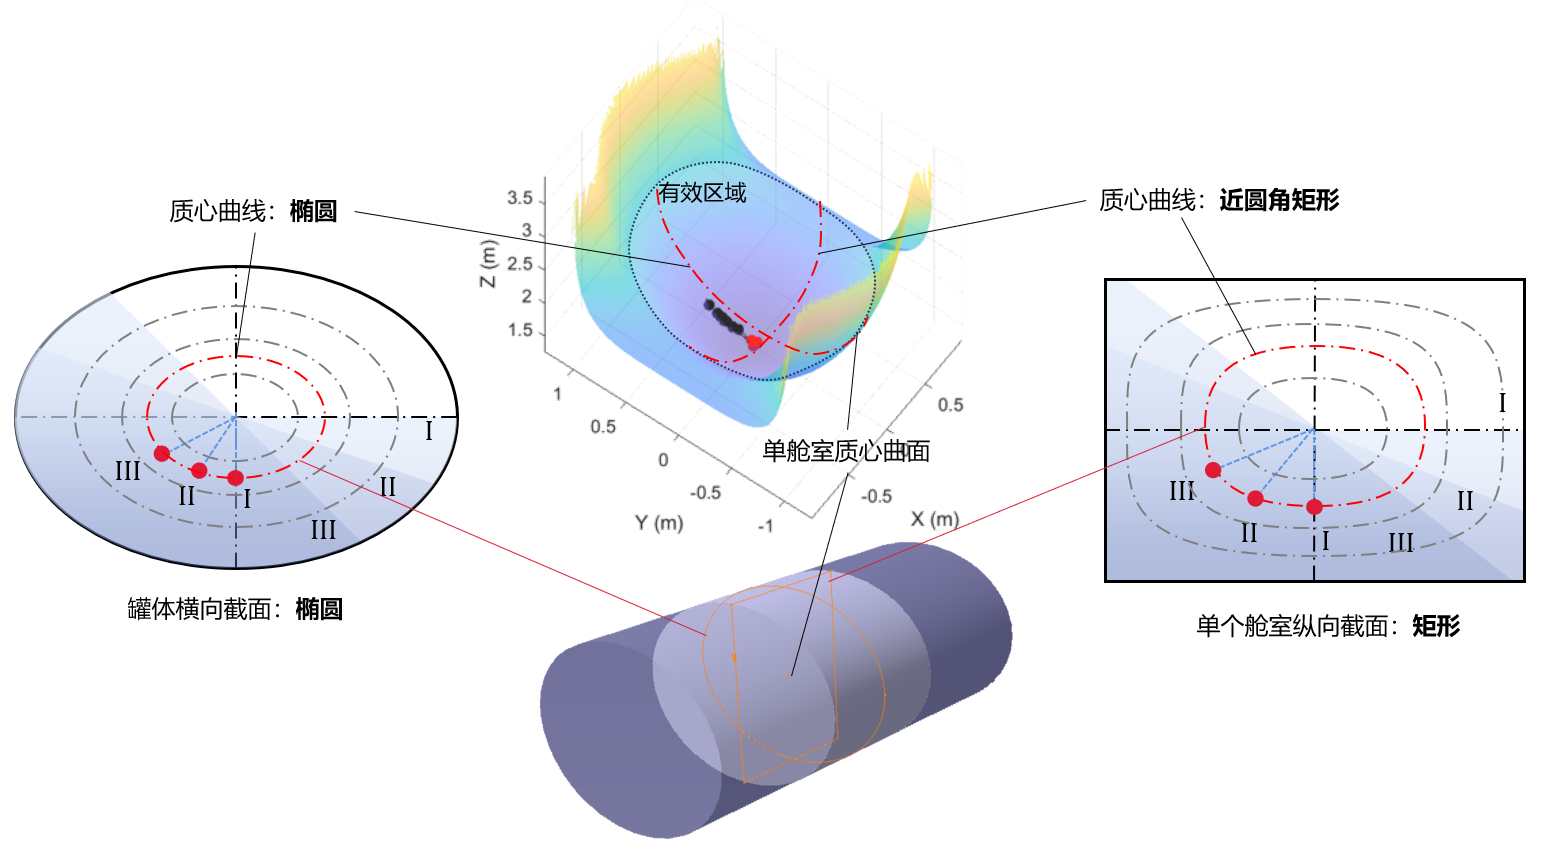
\includegraphics[width=1.0\linewidth]{fig/chap4/mass_surface.png}
            \caption{浴盆模型质心滑动平面设计}
            \label{fig:mass_surface}
            \end{figure}

            浴盆模型采用动力学方法求解集中质量在曲面上滑动时产生的输出力与力矩，该曲面即建模了在每个充液腔室内部液体晃动时其质心轨迹形成的曲面，虽输出力与力矩的表达式没有解析形式，但只要求曲面光滑且数值稳定性较高。


            本研究进一步细化方案，如图~\ref{fig:stl_model}所示，为表达液体在腔室间转移造成的稳态俯仰力矩，提出“滑动浴盆”模型，将浴盆模型中曲面的位置当做另一个集中质量在任意光滑曲线上滑动，该曲线建模了不同纵向稳态激励下罐内所有液体整体质心的轨迹。进一步，本研究提出了“滑动天平”模型，通过引入两个对称的浴盆来体现罐体绕Z轴旋转时产生的横摆力矩波动，并最终提出了“滑动伸缩天平”（Sliding Telescopic Libra, STL）模型，以进一步捕捉随液罐旋转而趋向于两侧的液体造成的横摆力矩稳态值的增加。

            \begin{figure}
            \centering
            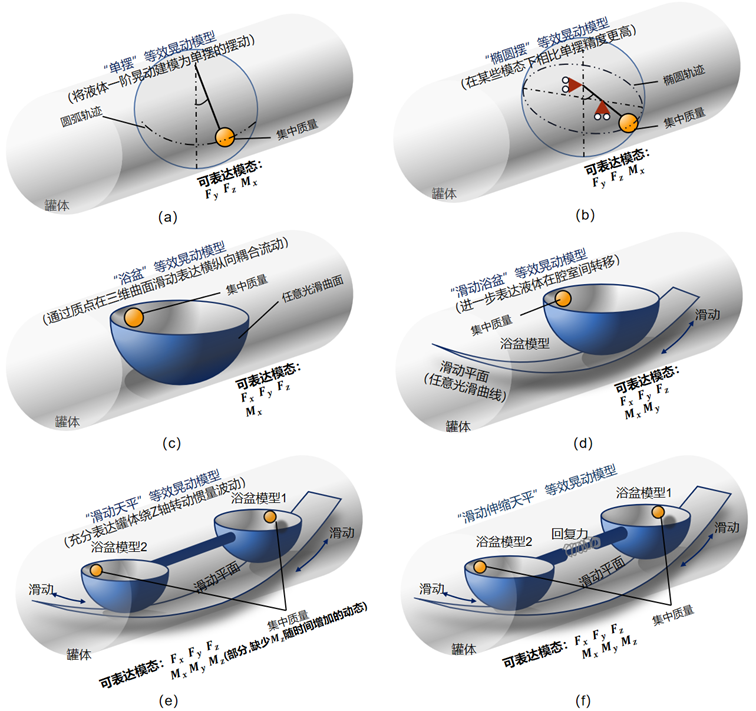
\includegraphics[width=1.0\linewidth]{fig/chap4/stl_model.png}
            \caption{滑动伸缩天平模型推导过程}
            \label{fig:stl_model}
            \end{figure}


            建立的STL模型作为非线性高精度机械等效扰动模型可表示为$\{\dot{x}_1, \dot{x}_1, Q_1\} = f_1(x_1,u|w_1)$，其中$x_1$为模型状态向量，$u$为模型输入激励向量，$w_1$为模型参数向量，$\dot{x}_1$为模型状态向量对时间的导数，$Q_1$为模型输出广义力；

            STL模型包含6个自由度，分别为两个浴盆各自内部小球的2个移动自由度$x_1,y_1$以及$x_2,y_2$，两个浴盆的共同滑动自由度$x_0$，以及两个浴盆之间的相对滑动自由度$d$；对应状态量共11个，如表~\ref{tab:stl_state}所示。所有状态量合称为$X_{STL}$。STL模型的参数包括18个，如表~\ref{tab:stl_param}所示，所有参数合称为$\boldsymbol{w_1}$。STL模型的输入包含6个维度，分别如表~\ref{tab:stl_input}所示。


            % 表2：STL模型状态变量定义
            \begin{table}[h]
            \centering
            \caption{STL模型状态变量定义}
            \label{tab:stl_state}
            \begin{tabular}{ccl}
            \toprule
            序号 & 状态符号 & 说明 \\
            \midrule
            1 & $x_0$ & 浴盆模型沿曲线的整体纵向位移 \\
            2 & $\dot{x_0}$ & 浴盆模型沿曲线的整体纵向位移速度 \\
            3 & $x_1$ & 浴盆1内小球的x向位移 \\
            4 & $y_1$ & 浴盆1内小球的y向位移 \\
            5 & $\dot{x_1}$ & 浴盆1内小球的x向速度 \\
            6 & $\dot{y_1}$ & 浴盆1内小球的y向速度 \\
            7 & $x_2$ & 浴盆2内小球的x向位移 \\
            8 & $y_2$ & 浴盆2内小球的y向位移 \\
            9 & $\dot{x_2}$ & 浴盆2内小球的x向速度 \\
            10 & $\dot{y_2}$ & 浴盆2内小球的y向速度 \\
            11 & $d$ & 两个浴盆模型的相对偏置距离 \\
            \bottomrule
            \end{tabular}
            \end{table}

            \begin{table}[h]
            \centering
            \caption{STL模型参数及其在充液率\SI{50}{\percent}时的识别结果}
            \label{tab:stl_param}
            \begin{tabular}{cclc}
            \toprule
            序号 & 参数名 & 说明 & 参数值（单位） \\
            \midrule
            1 & $k_{\alpha}$ & 浴盆曲面范数阶数 & 3.59 ($-$) \\
            2 & $k_{\sigma}$ & 浴盆曲面方形系数 & 7.71 ($-$) \\
            3 & $k_x$ & 浴盆曲面X轴范围 & 1.04 (m) \\
            4 & $k_y$ & 浴盆曲面Y轴范围 & 1.29 (m) \\
            5 & $k_z$ & 浴盆曲面Z轴范围 & 3.24 (m) \\
            6 & $h$ & 浴盆曲面底部净高 & 1.26 (m) \\
            7 & $a_p$ & 滑动平面曲线长半轴 & 15.5 (m) \\
            8 & $b_p$ & 滑动平面曲线短半轴 & 0.61 (m) \\
            9 & $p_r$ & 滑动平面曲线幂次 & 0.53 ($-$) \\
            10 & $m$ & 晃动部分质量 & 14498.66 (kg) \\
            11 & $c_{damp}$ & 小球晃动的阻尼系数 & 0.17 (s⁻¹) \\
            12 & $c_x$ & 浴盆X向移动阻尼系数 & 3.84 (s⁻¹) \\
            13 & $k_{a,dec}$ & 浴盆X向移动加速度换算系数 & 0.56 ($-$) \\
            14 & $s_{dev}$ & 浴盆曲面静态偏置距离 & 3.12 (m) \\
            15 & $k_{v,dec}$ & X向速度衰减系数 & 9.14 ($-$) \\
            16 & $k_{ax,pow}$ & X向加速度衰减系数 & 0.42 ($-$) \\
            17 & $a_{dev}$ & 浴盆曲面偏置的自衰减系数 & 0.20 (s⁻¹) \\
            18 & $b_{dev}$ & 浴盆曲面偏置的输入换算系数 & 0.12 (s⁻¹) \\
            \bottomrule
            \end{tabular}
            \end{table}


            

            % 表4：STL模型输入变量定义
            \begin{table}[h]
            \centering
            \caption{STL模型输入变量定义}
            \label{tab:stl_input}
            \begin{tabular}{cclc}
            \toprule
            序号 & 输入符号 & 说明 & 单位 \\
            \midrule
            1 & $a_x$ & 施加到罐体的纵向加速度 & $\mathrm{m/s^2}$ \\
            2 & $a_y$ & 施加到罐体的横向加速度 & $\mathrm{m/s^2}$ \\
            3 & $\phi$ & 罐体的侧倾角 & $\mathrm{rad}$ \\
            4 & $\ddot{\phi}$ & 罐体的侧倾角加速度 & $\mathrm{rad/s^2}$ \\
            5 & $\dot{\psi}$ & 罐体的横摆角速度 & $\mathrm{rad/s}$ \\
            6 & $\ddot{\psi}$ & 罐体的横摆角加速度 & $\mathrm{rad/s^2}$ \\
            \bottomrule
            \end{tabular}
            \end{table}

            STL模型可以用于和车辆动力学模型联合仿真，但模型的数学表达无法彻底解析化，而是通过数值方式来表达其计算过程的。首先定义一个三维空间中的曲面$F$作为浴盆，$z = F(x, y)$，$F$要求连续可微；同时定义一个二维空间中的曲线$C$作为钢丝，$z = C(x)$。在第$k$个时刻，通过如下方式描述两个浴盆同时沿着空间中曲线的滑动情况：

            定义第$k$时刻下曲线的切向量$\vec{t}_k$（默认方向的）以及法向量$\vec{n}_k$
            \begin{equation}
            C_1 = \frac{\mathrm{d}C(x)}{\mathrm{d}x}\bigg|_{x=x_{0,k}}, \vec{t}_k = \frac{1}{\sqrt{1 + C_1^2}}[1, C_1], \vec{n}_k = \frac{1}{\sqrt{1 + C_1^2}}[C_1, -1]
            \end{equation}

            每个时刻作用于两个浴盆共同质心上的加速度是实际$\mathrm{x}$方向加速度$a_x$和垂向的重力加速度$-g$经过非线性化映射后的结果。
            \begin{equation}
            \vec{a}_k' = \begin{bmatrix} k_{a,dec} a_{x,k}^{k_{ax,pow}} \\ -g \end{bmatrix}
            \end{equation}

            \begin{figure}
            \centering
            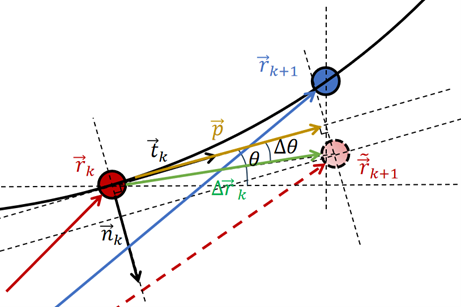
\includegraphics[width=0.5\linewidth]{fig/chap4/sliding_lumped_mass.png}
            \caption{二维曲线/三维曲面上滑动质点建模}
            \label{fig:sliding_lumped_mass}
            \end{figure}

            假定两个浴盆的质心不受曲线约束，而是可以在二维平面上自由移动，那么利用运动学公式可以简单计算出自由运动时两盆质心的位置$\vec{\tilde{r}}_{k+1}$，以及此时相对于上一时刻真实位置的增量$\Delta \vec{r}_k$。具体计算过程示意图如图~\ref{fig:sliding_lumped_mass}所示。

            \begin{equation}
            \vec{\tilde{r}}_{k+1} = \vec{r}_k + \vec{v}_k' \Delta t + \frac{1}{2} \vec{a}_k' (\Delta t)^2, ~\Delta \vec{r}_k = \vec{\tilde{r}}_{k+1} - \vec{r}_k
            \end{equation}

            \begin{equation}
            \theta_k = \tan^{-1} \frac{\mathrm{d}C(x)}{\mathrm{d}x}\bigg|_{x_{0,k}}, ~
            \Delta \theta_k = \mathrm{sign}(\dot{\vec{n}}_k \cdot \Delta \vec{r}_k) \cos^{-1} \frac{\vec{t}_k \cdot \Delta \vec{r}_k}{\|\vec{t}_k\| \|\Delta \vec{r}_k\|}
            \end{equation}

            \begin{equation}
            x_{0,k+1} = \vec{r}_{1,k} - \|\Delta \vec{r}_k\| \sin \Delta \theta_k \sin \theta_k,~
            z_{0,k+1} = C(x_{0,k+1}) ,~ \vec{r}_{k+1} = \begin{bmatrix} x_{0,k+1} \\ z_{0,k+1} \end{bmatrix}
            \end{equation}

            \begin{equation}
            v_{k+1}' = (1 - c_x \Delta t) \frac{\vec{r}_{k+1} - \vec{r}_k}{\Delta t}
            \end{equation}

            再对每个浴盆的分离情况进行更新：
            \begin{equation}
            d_{k+1} = s_{dev} + (1 - k_{a,dev} \Delta t)(d_k - s_{dev}) + k_{b,dev} \Delta t |\dot{\psi}_k|
            \label{eq:d_dev}
            \end{equation}

            再对每个浴盆内质点的运动情况进行更新：$z_{1,k} = F(x_{1,k}, y_{1,k})$
            \begin{equation}
            \vec{n}_k = \nabla(F(x,y) - z)
            \end{equation}

            滑动质心位置向量$\vec{r}_k$的第一个分量中，两个浴盆模型分别取$d_k$为+和-。
            \begin{equation}
            \vec{r}_k = \begin{bmatrix} x_{0,k} + x_{1,k} \pm d_k \\ y_{1,k} \\ z_{0,k} + z_{1,k} \end{bmatrix}
            \label{eq:stl_state_prime}
            \end{equation}

            将旋转部分的输入转换为
            \begin{equation}
            a_k = \begin{bmatrix} a_{x,k} - \ddot{\psi}_k \vec{r}_k \cdot \vec{j} \\ a_{y,k} \cos \phi_k - a_{z,k} \sin \phi_k + \ddot{\psi}_k \vec{r}_k \cdot \vec{i} - \ddot{\phi}_k \vec{r}_k \cdot \vec{k} \\ a_{y,k} \sin \phi_k + a_{z,k} \cos \phi_k + \ddot{\phi}_k \vec{r}_k \cdot \vec{j} \end{bmatrix}
            \end{equation}

            \begin{equation}
            \vec{\tilde{r}}_{k+1} = \vec{r}_k + \vec{v}_k \Delta t + \frac{1}{2} \vec{a}_k (\Delta t)^2, ~\Delta \vec{r}_k = \vec{\tilde{r}}_{k+1} - \vec{r}_k
            \end{equation}

            \begin{equation}
            \vec{p} = \Delta \vec{r}_k - (\Delta \vec{r}_k \cdot \vec{n}) \frac{\vec{n}}{\|\vec{n}\|}
            \end{equation}

            \begin{equation}
            \begin{aligned}
            x_{1,k+1} &= (\vec{r}_k + \vec{p}) \cdot \vec{i} \\
            y_{1,k+1} &= (\vec{r}_k + \vec{p}) \cdot \vec{j} \\
            z_{1,k+1} &= F(x_{1,k+1}, y_{1,k+1}) \end{aligned},\quad
            \vec{r}_{k+1} = \begin{bmatrix} x_{1,k+1} \\ y_{1,k+1} \\ z_{1,k+1} \end{bmatrix}
            \label{eq:stl_state}
            \end{equation}

            关于浴盆曲面$z = F(x,y)$以及整体滑动曲线$z = C(x)$的定义，可以参考下面的例子：
            \begin{equation}
            z = F(x,y) = \mathrm{Re}\left( -k_z \left( 1 - \left| \frac{x}{k_x} \right|^a - \left| \frac{y}{k_y} \right|^a \right)^{\frac{1}{a}} \right) + k_z + h
            \end{equation}
            \noindent 其中，$a = 2 + k_\alpha |x_0|^{k_e}$，$\mathrm{Re}(\cdot)$表示取实部。

            \begin{equation}
            z = \mathrm{Re}\left( -b_p \mathrm{sign}(a_p - |x|) \left( 1 - \left( \frac{x}{a_p} \right)^2 \right) \right)
            \end{equation}

            实际上只需要保证这两个函数对输入量分别连续可导即可，并不需要完全按照给定的形式。不过需要注意的是，当调整了滑动曲面和/或曲线的表达结构后，STL模型的参数定义也需要进行相应修改，可以通过这种方式简化或进一步扩展STL模型。

        \subsubsection{模型参数辨识}
            \label{subsub:model_identification}
            滑动伸缩天平模型的参数需要利用CFD仿真数据进行识别校准。首先从罐体的6个空间自由度中选择关注的几个自由度$N_1 \subseteq \{d_x\ d_y\ d_z\ \theta_x\ \theta_y\ \theta_z\}$，其中$d_i$和$\theta_i$分别表示对应坐标轴正方向的平动和转动自由度，以及相应自由度激励的范围。编制正交工况表$L_{N^T}(m_1^{n_1}m_2^{n_2}\dots m_p^{n_p})$，其中$N^T$为所需的正交工况个数，$m_i,n_i$分别表示第$i$组的水平数和因素个数，$\sum_{i=1}^p n_i = N_1$；

            本研究选取关心的自由度为$M_1 = \{d_x\ d_y\ \theta_x\ \theta_z\}$，即沿着$x$和$y$轴的平动激励以及绕着$x$和$z$轴的转动激励，因为在液罐车行驶过程中纵向加速度以及侧倾、横摆激励是最常见的。针对这四个方向的不同强度激励，制定包含$n=16$组工况的正交工况表$L_{16}(4^4)$。考虑在行驶过程中经常出现的对液罐的4个激励来源：纵向加速度$a_x$、侧向加速度$a_y$、侧倾角加速度$\ddot{\phi}$、横摆角加速度$\ddot{\psi}$，并各自离散为4个档：$a_x$:0,1,3,5$\mathrm{m/s^2}$，$a_y$:0,1,3,5$\mathrm{m/s^2}$，$\ddot{\phi}$:0,0.25,0.5,1$\mathrm{rad/s^2}$，$\ddot{\psi}$:0,0.25,0.5,1$\mathrm{rad/s^2}$，用以设计$L_{16}(4^4)$标准正交工况表，如表~\ref{tab:orthogonal_conditions}所示。

            % 表1：正交工况表（1~8与9~16并列）
            \begin{table}[h]
            \centering
                \begin{threeparttable}[c]
                \caption{正交工况表}
                \label{tab:orthogonal_conditions}
                \begin{tabular}{ccccc|ccccc}
                \toprule
                标号 & $a_x$ & $a_y$ & $\ddot{\phi}$ & $\ddot{\psi}$ & 标号 & $a_x$ & $a_y$ & $\ddot{\phi}$ & $\ddot{\psi}$ \\
                \midrule
                1 & 0 & 0 & 0 & 0 & 9 & 3 & 0 & 0.5 & 1 \\
                2 & 0 & 1 & 0.25 & 0.25 & 10 & 3 & 1 & 1 & 0.5 \\
                3 & 0 & 3 & 0.5 & 0.5 & 11 & 3 & 3 & 0 & 0.25 \\
                4 & 0 & 5 & 1 & 1 & 12 & 3 & 5 & 0.25 & 0 \\
                5 & 1 & 0 & 0.25 & 0.5 & 13 & 5 & 0 & 1 & 0.25 \\
                6 & 1 & 1 & 0 & 1 & 14 & 5 & 1 & 0.5 & 0 \\
                7 & 1 & 3 & 1 & 0 & 15 & 5 & 3 & 0.25 & 1 \\
                8 & 1 & 5 & 0.5 & 0.25 & 16 & 5 & 5 & 0 & 0.5 \\
                \bottomrule
                \end{tabular}
                \begin{tablenotes}
                    \item 上述4个激励物理量单位分别为$a_x$、$a_y$:$\mathrm{m/s^2}$，$\ddot{\phi}$、$\ddot{\psi}$:$\mathrm{rad/s^2}$
                \end{tablenotes}
                \end{threeparttable}
            \end{table}

    

            为进行CFD仿真获取高精度模型力特性值，建立罐体的精细计算流体动力学模型，符号表示为$g_0(t) = f_0(u(t))$，其中$u(t)$为模型输入激励向量时间序列，$g_0(t)$为模型输出广义力时间序列。本文中选择CFD仿真软件StarCCM+作为计算流体动力学建模的平台，其中一组工况的仿真过程如图~\ref{fig:cfd_illust}所示。液体晃动CFD仿真模型与车液耦合联合仿真平台搭建在\ref{sub:cosim_platform}节将详细展开。

            \begin{figure}
            \centering
            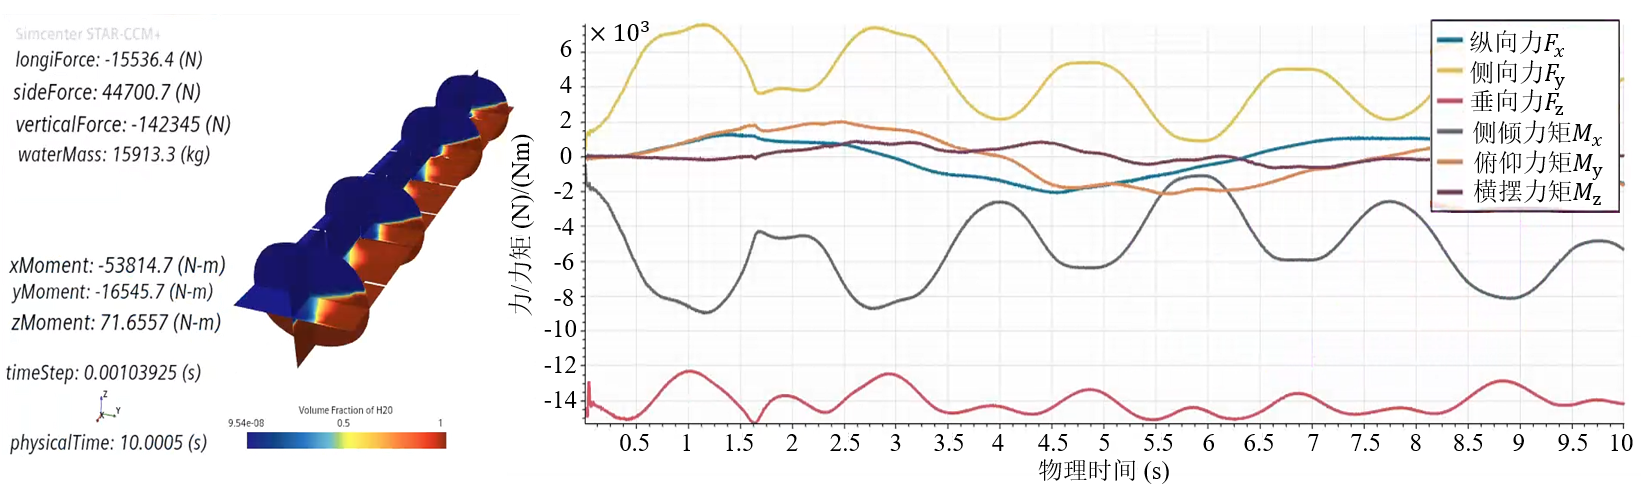
\includegraphics[width=1.0\linewidth]{fig/chap4/cfd_illust.png}
            \caption{CFD仿真过程示意}
            \label{fig:cfd_illust}
            \end{figure}

            利用正交工况表$L_{N^T}(m_1^{n_1}m_2^{n_2}\dots m_p^{n_p})$为精细计算流体力学模型$f_0$设置阶跃输入$U(t)$，建立CFD仿真数据库$D_{CFD}$，通过遗传算法进行参数辨识，最小化仿真时域内STL模型预测结果与CFD仿真结果的累计均方误差，代价函数为加权的16工况下CFD仿真输出力/力矩序列和模型输出力/力矩序列距离的二范数：
            \begin{equation}
            J = \sum_{\text{case}=1}^{16} \left(\begin{aligned} w_{F_x}\|F_x - F_{x0}\|_2^2 + w_{F_y}\|F_y - F_{y0}\|_2^2 + w_{F_z}\|F_z - F_{z0}\|_2^2 \\+ w_{M_x}\|M_x - M_{x0}\|_2^2 + w_{M_y}\|M_y - M_{y0}\|_2^2 + w_{M_z}\|M_z - M_{z0}\|_2^2\end{aligned} \right)
            \end{equation}

            \begin{figure}[h]
            \centering
            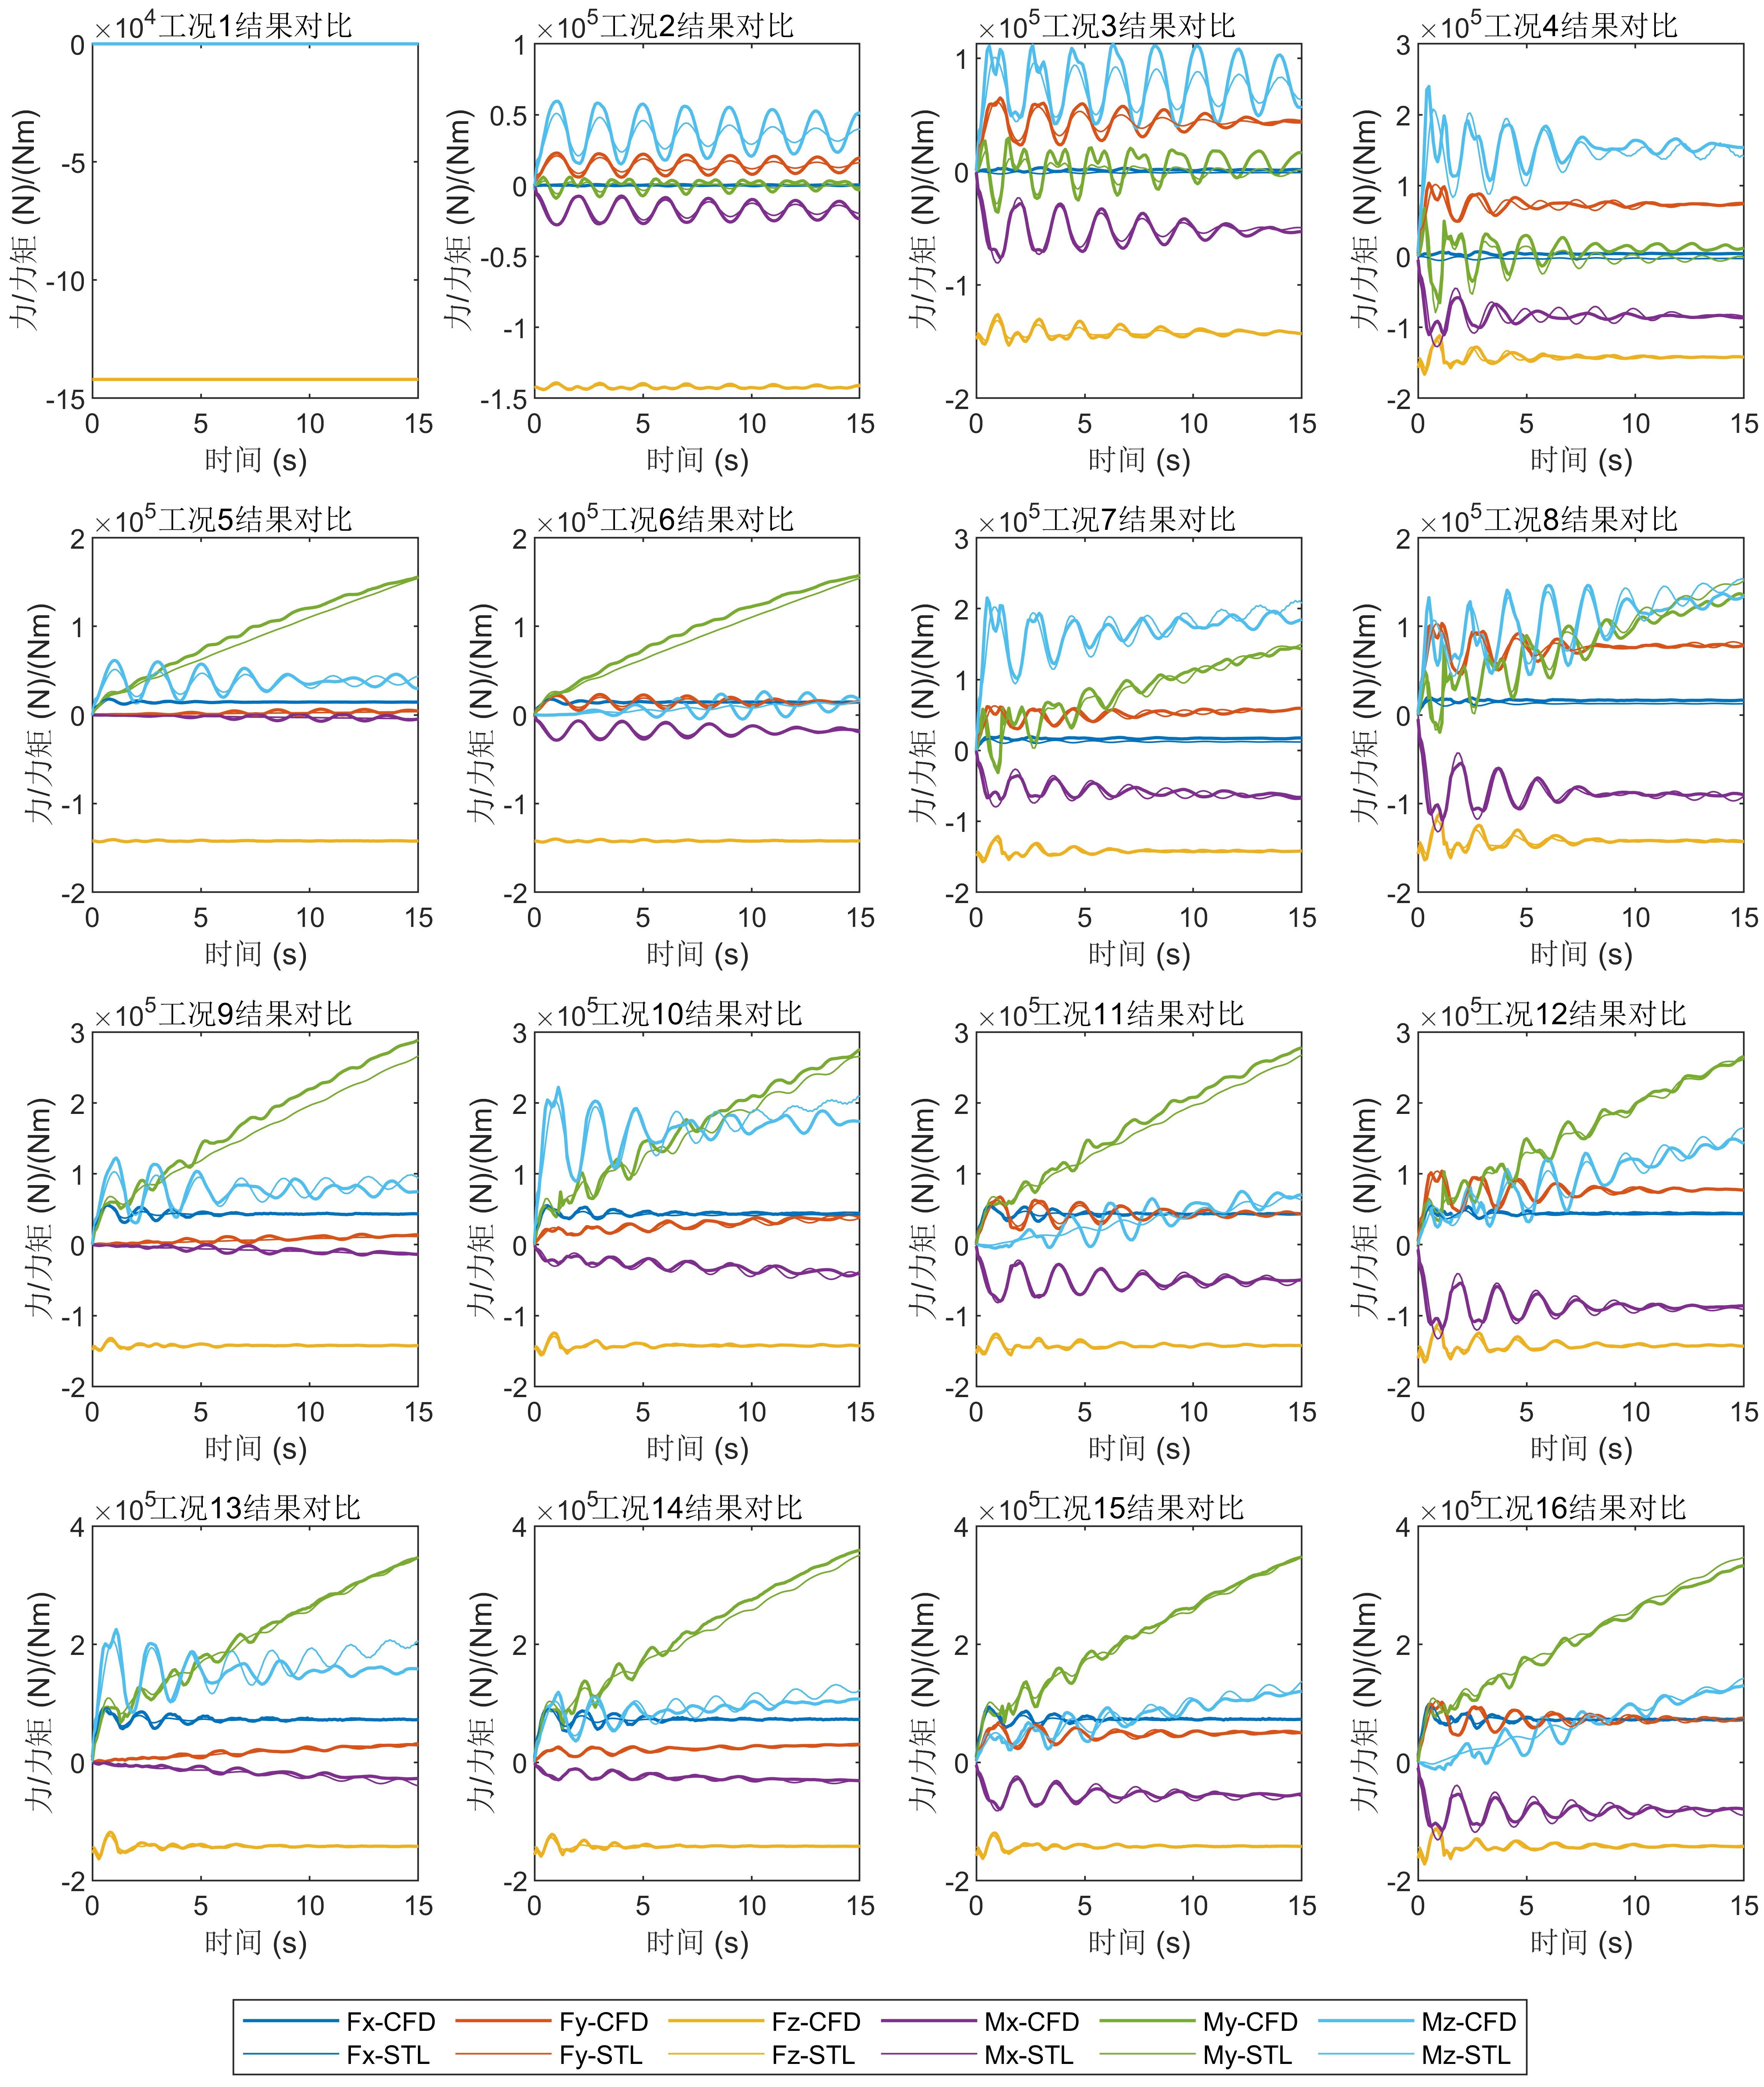
\includegraphics[width=1.0\linewidth]{fig/chap4/compare_all_cases.png}
            \caption{16组工况下STL模型与CFD仿真结果对比}
            \label{fig:compare_all_cases}
            \end{figure}

            对\SI{50}{\percent}充液率罐体的滑动伸缩天平模型参数进行识别得到，如表~\ref{tab:stl_param}所示。所有16组仿真工况结果如图~\ref{fig:compare_all_cases}所示，其中粗线表示CFD数据，细线为STL模型在相同输入激励下的预测结果。可以看出，在空间内所有6个自由度的力/力矩输出上，STL模型都与CFD仿真保持了相同的趋势和相似的细节；相比于二维模型，不仅首次捕捉到包含纵向的横纵耦合晃动，还捕捉到了横摆晃动及俯仰力矩$M_y$随舱室间液体转移而产生的稳态变化。此外，与CFD仿真单个工况动辄数小时的计算时间相比，STL模型在MATLAB中对未来\SI{15}{s}的预测仅需\SI{5}{ms}，经过C++编译后可达到小于\SI{1}{ms}的速度，实现超实时、高精度快速仿真。






            
   



    \subsection{残差强化学习重线性化}
        \label{sub:residual_rl_relinearization}
        STL模型精度较高且能够实时快速仿真，但由于其非解析特性，难以直接应用于在线优化的模型预测控制。为了将STL模型用于在线优化，需要对STL模型进行实时\emph{重线性化}（relinearization）处理，即根据当前STL模型的实时状态，获得结构更简单、力特性具有解析表达式的等效模型状态与参数。该等效模型与STL结构不同，精度相对受限，但更适合在线优化求解。本节以基础模型加可学习残差模型的形式进行模型重线性化与状态估计，首先介绍相较于STL模型更加简化的线性双摆模型（Linearized Dual Pendulum, LDP），以及通过强化学习方式进行的残差模型训练与效果验证。

        \subsubsection{线性双摆模型}
            \label{subsub:ldp}
            LDP模型相比STL将更加简化，为实时计算所关注的自由度将更少。选择最关注的自由度$\mathcal{N}_2 \subseteq \mathcal{N}_1$，并建立线性化等效双摆模型$[\dot{\Theta}, Q_2] = f_2(\Theta, u|w_2)$，其中$\Theta$为模型状态向量，$u$为模型输入激励向量，$w_2$为模型参数向量，$\dot{\Theta}$为模型状态向量对时间的导数，$Q_2$为模型输出广义力；LDP包含两个既有侧向加速度又有侧倾角加速度输入的单摆模型，沿车辆轴线分布，其中任意一个单摆如图~\ref{fig:sp_illust}所示，涉及的坐标系定义如图~\ref{fig:coord_def}所示。

            \begin{figure}
            \centering
            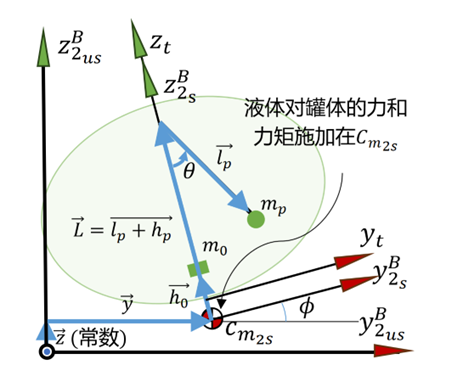
\includegraphics[width=0.5\linewidth]{fig/chap4/sp_illust.png}
            \caption{带侧倾输入的单摆模型示意}
            \label{fig:sp_illust}
            \end{figure}

            先考虑单个摆的情况，集中质量$m_0$与$m_p$的位置向量如下：
            \begin{equation}
            \vec{R}_{p0} = \vec{y} + \vec{h_0} = (x_0 + x_{1|2} \pm d)\vec{i} + (y - h_0 \sin \phi)\vec{j} + (h_0 \cos \phi)\vec{k}
            \end{equation}
            \begin{equation}
            \begin{aligned}
            \vec{R}_p &= \vec{y} + \vec{L} + \vec{h_p} \\
            &= (x_0 + x_{1|2} \pm d)\vec{i} + (y - L \sin \phi + l_p \sin(\phi + \theta))\vec{j} + (L \cos \phi - l_p \cos(\phi + \theta))\vec{k}
            \end{aligned}
            \end{equation}
            紧接着，对其进行微分以获得两个集中质量的速度向量：
            \begin{equation}
            \dot{\vec{R}}_{p0} = (\dot{y} - h_0 \dot{\phi} \cos \phi)\vec{j} + (-h_0 \dot{\phi} \sin \phi)\vec{k}
            \end{equation}
            \begin{equation}
            \begin{aligned}
            \dot{\vec{R}}_p &= \left[ \dot{y} - \left(L \cos \phi + l_p \cos(\phi + \theta)\right)\dot{\phi} + l_p \dot{\theta} \cos(\phi + \theta) \right]\vec{j} \\
            &\quad + \left[ \left(-L \sin \phi + l_p \sin(\phi + \theta)\right)\dot{\phi} + l_p \dot{\theta} \sin(\phi + \theta) \right]\vec{k}
            \end{aligned}
            \end{equation}
            再次微分得到加速度向量：
            \begin{equation}
            \ddot{\vec{R}}_{p0} = \left[ \ddot{y} - \ddot{\phi} h_0 \cos \phi + \dot{\phi}^2 h_0 \sin \phi \right]\vec{j} + \left[ -\ddot{\phi} h_0 \sin \phi - \dot{\phi}^2 h_0 \cos \phi \right]\vec{k}
            \end{equation}
            \begin{equation}
            \begin{aligned}
            \ddot{\vec{R}}_p &= \begin{bmatrix}
            \ddot{y} + \ddot{\phi}\left[-L \cos \phi + L_p \cos(\phi + \theta)\right] + \ddot{\theta} l_p \cos(\phi + \theta) \\
            +\dot{\phi}^2\left[L \sin \phi - l_p \sin(\phi + \theta)\right] + \dot{\theta}^2\left[-l_p \sin(\phi + \theta)\right] \\
            -2\dot{\phi}\dot{\theta} l_p \sin(\phi + \theta)
            \end{bmatrix}\vec{j} \\
            &\quad + \begin{bmatrix}
            \ddot{\phi}\left[-L \sin \phi + L_p \cos(\phi + \theta)\right] + \ddot{\theta} l_p \sin(\phi + \theta) \\
            +\dot{\phi}^2\left[L \cos \phi - l_p \cos(\phi + \theta)\right] + \dot{\theta}^2\left[-l_p \cos(\phi + \theta)\right] \\
            -2\dot{\phi}\dot{\theta} l_p \cos(\phi + \theta)
            \end{bmatrix}\vec{k}
            \end{aligned}
            \end{equation}
            当我们选择$y_{2us}^B o_{2us}^B z_{2us}^B$平面（请参见图~\ref{fig:coord_def}）为零势能面，则动能$T$与势能$U$可以被表示为：
            \begin{equation}
            T = \frac{1}{2}m_p\left( \left(\dot{\vec{R}}_p \cdot \vec{j}\right)^2 + \left(\dot{\vec{R}}_p \cdot \vec{k}\right)^2 \right) + \frac{1}{2}m_0\left( \left(\dot{\vec{R}}_{p0} \cdot \vec{j}\right)^2 + \left(\dot{\vec{R}}_{p0} \cdot \vec{k}\right)^2 \right)
            \end{equation}
            \begin{equation}
            U = m_p g \left[ L \cos \phi - l_p \cos(\phi + \theta) \right]
            \end{equation}
            根据欧拉-拉格朗日方程：
            \begin{equation}
            \frac{d}{dt}\frac{\partial T}{\partial \dot{\theta}} - \frac{\partial T}{\partial \theta} + \frac{\partial U}{\partial \theta} = 0
            \end{equation}
            摆动自由度$\theta$的动态微分方程推导如下：
            \begin{equation}
            \ddot{\theta} + \frac{1}{l_p} \ddot{y} \cos(\phi + \theta) + \ddot{\phi}\left[ \left(1 - \frac{h_p}{l_p}\right)\cos\theta + 1 \right] - \dot{\phi}^2 \left(1 - \frac{h_p}{l_p}\right)\sin\theta + \frac{g}{l_p}\sin(\phi + \theta) + c_d \dot{\theta} = 0
            \end{equation}
            罐体所受的侧向力$F_y$和力矩$M_x$为：
            \begin{equation}
            F_y = -\left(m_0 \ddot{\vec{R}}_{p0} + m_p \ddot{\vec{R}}_p\right) \cdot \vec{j}
            \end{equation}
            \begin{equation}
            M_x = m_0\left[ \vec{R}_{p0} \cdot \vec{k} \ddot{\vec{R}}_{p0} \cdot \vec{j} - \vec{R}_{p0} \cdot \vec{j} \left( \ddot{\vec{R}}_{p0} \cdot \vec{k} + g \right) \right] + m_p\left[ \vec{R}_p \cdot \vec{k} \ddot{\vec{R}}_p \cdot \vec{j} - \vec{R}_p \cdot \vec{j} \left( \ddot{\vec{R}}_p \cdot \vec{k} + g \right) \right]
            \end{equation}
            \begin{equation}
            M_z = m_0\left[ \vec{R}_{p0} \cdot \vec{j} \ddot{\vec{R}}_{p0} \cdot \vec{i} - \vec{R}_{p0} \cdot \vec{i} \ddot{\vec{R}}_{p0} \cdot \vec{j} \right] + m_p\left[ \vec{R}_p \cdot \vec{j} \ddot{\vec{R}}_p \cdot \vec{i} - \vec{R}_p \cdot \vec{i} \ddot{\vec{R}}_p \cdot \vec{j} \right]
            \end{equation}
            代入上述位置与加速度向量具体展开并保留线性项为：
            \begin{equation}
            F_y = -(m_p + m_0)v_{x2}\left(\ddot{\beta}_2 + \dot{\psi}_2\right) + (m_0 h_0 + m_p h_p)\ddot{\phi}_2 - m_p l_p \ddot{\theta}
            \end{equation}
            \begin{equation}
            \begin{aligned}
            M_x &= v_{x2}(m_0 h_0 + m_p h_p)\left(\ddot{\beta}_2 + \dot{\psi}_2\right) - \left(m_0 h_0^2 + m_p h_p^2\right)\ddot{\phi}_2 \\
            &\quad + (m_0 h_0 + m_p h_p)g \phi_2 + m_p h_p l_p \ddot{\theta} - m_p l_p g \theta
            \end{aligned}
            \end{equation}
            \noindent 其中，对一般的单摆，侧向加速度$\ddot{y} = \dot{v}_{y2} + \dot{\psi}_2 v_{x2}$。当存在两个摆模型时，其摆动自由度可以分别被命名为$\theta_1$和$\theta_2$。两者均适用于上述方程。对于两个自由度$\theta_1$和$\theta_2$而言，其在式\eqref{eq:single_pendulum_ddtheta}上的区别仅仅在于侧向加速度$\ddot{y}$的输入。
            \begin{equation}
            \ddot{\theta} + \frac{1}{l_p} \ddot{y} - \frac{h_p}{l_p} \ddot{\phi}_2 + \frac{g}{l_p} \theta + \frac{g}{l_p} \phi_2 + c_d \dot{\theta} \approx 0
            \label{eq:single_pendulum_ddtheta}
            \end{equation}
            此外，还需要加上一个分离自由度$d$如式\eqref{eq:d_dev}。可以通过增加一个输入量的形式来考虑这个自由度，或者在重线性化时丢弃这个自由度将其影响转换为对其他参数的改变。由于其中包含非线性的绝对值项，所以无法将其直接线性化用于MPC控制，但是可以采用引入新的输入变量$u_k$的方式来代替$|\dot{\psi}_k|$，需要同时加入约束来保证其等价性：
            \begin{equation}
             -\dot{\psi}_k \leq u_k \leq \dot{\psi}_k
            \end{equation}
            同时在MPC的优化函数中加入$R\|u_k\|_2^2$，通过调节$R$可以控制最优解中$u_k$逼近$|\dot{\psi}_k|$的精度。但是本方法会使求解的输入变量数量翻倍，对求解时间产生一定负面影响，但影响相对有限。平均而言，输入变量增加一倍会使求解时间增加约\SIrange{20}{30}{\percent}；而预测时域减小一半，则可以降低求解时间\SI{50}{\percent}以上。

            对于前后2个浴盆的侧向加速度变成了，增加了一个横摆角速度项：
            \begin{equation}
            \begin{aligned}
            \ddot{y}_1 &= v_{x2}\ddot{\beta}_2 + v_{x2}\dot{\psi}_2 + \ddot{\psi}_2 (x_0 + x_1 + d) \approx v_{x2}\ddot{\beta}_2 + v_{x2}\dot{\psi}_2 + \ddot{\psi}_2 (x_0 + d) \\
            \ddot{y}_2 &= v_{x2}\ddot{\beta}_2 + v_{x2}\dot{\psi}_2 + \ddot{\psi}_2 (x_0 + x_2 - d) \approx v_{x2}\ddot{\beta}_2 + v_{x2}\dot{\psi}_2 + \ddot{\psi}_2 (x_0 - d)
            \end{aligned}
            \label{eq:ddyaw_input}
            \end{equation}
            令$x_1 = x_0 + d$以及$x_2 = x_0 - d$，将其代入侧向力和侧倾力矩的表达式中：
            \begin{equation}
            \begin{aligned}
            \ddot{\theta}_1 + \frac{1}{l_p} \ddot{y}_1 + \left(2 - \frac{h_p}{l_p}\right)\ddot{\phi}_2 + \frac{g}{l_p}(\phi_2 + \theta_1) + c_d \dot{\theta}_1 &= 0 \\
            \ddot{\theta}_2 + \frac{1}{l_p} \ddot{y}_2 + \left(2 - \frac{h_p}{l_p}\right)\ddot{\phi}_2 + \frac{g}{l_p}(\phi_2 + \theta_2) + c_d \dot{\theta}_2 &= 0
            \end{aligned}
            \end{equation}
            \begin{equation}
            \begin{aligned}
            F_{y1} &= \frac{1}{2}\left[ -(m_p + m_0)\left(v_{x2}\ddot{\beta}_2 + v_{x2}\dot{\psi}_2 + x_1 \ddot{\psi}_2\right) + (m_0 h_0 + m_p h_p)\ddot{\phi}_2 - m_p l_p \ddot{\theta}_1 \right] \\
            F_{y2} &= \frac{1}{2}\left[ -(m_p + m_0)\left(v_{x2}\ddot{\beta}_2 + v_{x2}\dot{\psi}_2 + x_2 \ddot{\psi}_2\right) + (m_0 h_0 + m_p h_p)\ddot{\phi}_2 - m_p l_p \ddot{\theta}_2 \right]
            \end{aligned}
            \end{equation}
            \begin{equation}
            \begin{aligned}
            M_x &= (m_0 h_0 + m_p h_p)\left(v_{x2}\ddot{\beta}_2 + v_{x2}\dot{\psi}_2 + x_0 \ddot{\psi}_2\right) - \left(m_0 h_0^2 + m_p h_p^2\right)\ddot{\phi}_2 \\
            &\quad + (m_0 h_0 + m_p h_p)g \phi_2 + \frac{1}{2}m_p h_p l_p (\ddot{\theta}_1 + \ddot{\theta}_2) - \frac{1}{2}m_p l_p g (\theta_1 + \theta_2)
            \end{aligned}
            \end{equation}
            \begin{equation}
            \begin{aligned}
            M_z &= F_{y1}(x_0 + d) - F_{y2}(x_0 - d) \\
            &= \frac{1}{2}(m_p + m_0)(x_2 - x_1)v_{x2}\left(\ddot{\beta}_2 + \dot{\psi}_2\right) + \frac{1}{2}(m_p + m_0)(x_2^2 - x_1^2)\ddot{\psi}_2 \\
            &\quad + \frac{1}{2}(x_1 - x_2)(m_0 h_0 + m_p h_p)\ddot{\phi}_2 + \frac{1}{2}m_p l_p (x_2 \ddot{\theta}_2 - x_1 \ddot{\theta}_1)
            \end{aligned}
            \end{equation}
            LDP模型一共包含2个自由度$\theta_1$与$\theta_2$，包含7个参数，分别为：$h_0\ h_p\ l_p\ m_0\ x_0\ d\ c_d$。模型一共包含3个输出，分别为$F_y\ M_x\ M_z$，输入为$\ddot{y}\ \ddot{\psi}\ \ddot{\phi}\ \phi$。

            利用CFD数据$D_{CFD}$采用启发式算法按STL模型相同步骤标定线性化等效双摆模型$f_2$的参数初值$w_{20}$；上述线性化等效摆模型为$N \geq 1$个单摆的线性组合（$N \geq 1$）。对于本文采用的LDP而言，$N=2$；也可以加入纵向的线性化摆进行组合，如三摆模型（双摆模型+纵向一个线性化摆）及其他选择。


            \begin{figure}
            \centering
            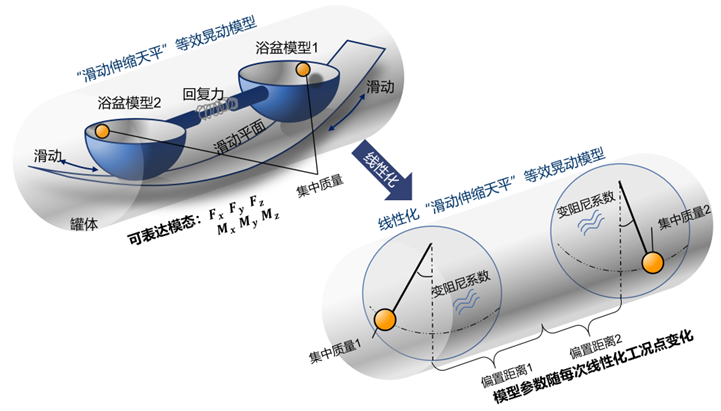
\includegraphics[width=0.9\linewidth]{fig/chap4/linearize_illust.png}
            \caption{将滑动质点模型实时重线性化为线性双摆模型}
            \label{fig:linearize_illust}
            \end{figure}

        \subsubsection{残差重线性化模型训练}    
            \label{subsub:putty_model}

            模型重线性化的示意图如图~\ref{fig:linearize_illust}所示，其核心是根据STL模型的状态量得到合适的LDP模型参数变化量和状态值。但由于LDP模型与STL模型结构完全不同，传统线性化方法如Jacobian线性化等在LDP模型中无法直接应用，故需要采用其他方法实现模型重线性化。
            

            具体而言，本文采用\emph{模型补土}（putty model）或\emph{残差模型}（residual model）的思想得到合适的参数变化量，以更加精确地线性化STL模型。训练神经网络$[\Theta,\Delta w_2] = n(x_1)$，其中第二个输出为LDP参数$w_2$的变化量$\increment w_2$，将线性模型难以反映的动态在所关注的几秒钟内体现在参数中。训练方案如图~\ref{fig:residual_learning}所示。
            
            采用STL模型而非直接用CFD计算结果作为真值的原因在于两点：首先，CFD计算速度慢，用于模型训练的成本过高；其次，CFD结果难以用数量较少的状态量简洁描述当前状态，因此需要一个具有有限状态、精度较高且可以快速计算的模型来表征当前液体状态。这也是STL模型存在的意义。STL模型还可用于控制算法联合快速验证仿真，作为初步验证模型；验证通过后，再进行CFD联合仿真，通过更精确的模型进一步验证。





            \begin{figure}
            \centering
            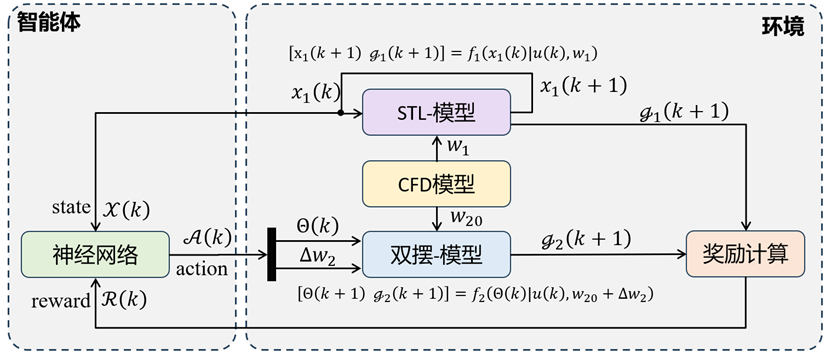
\includegraphics[width=0.9\linewidth]{fig/chap4/residual_learning.png}
            \caption{利用强化学习方法训练残差神经网络进行状态观测}
            \label{fig:residual_learning}
            \end{figure}

            将STL模型表述为黑盒输入输出形式：
            \begin{equation}
            [X(k+1),~Q_1(k+1)] = f_1(X(k),u(k)|w_1)
            \end{equation}
            将LDP模型表示为线性状态空间方程的形式：
            \begin{equation}
            [\Theta(k+1),~ Q_2(k)] = f_2(\Theta(k),u(k)|w_2) = \begin{cases}
            A|_{w_2} \Theta(k) + B|_{w_2} u(k) \\
            Q_2(k) = C|_{w_2} \Theta(k) + D|_{w_2} u(k)
            \end{cases}
            \end{equation}
            使其在每次需要重线性化模型时，在基础线性化参数$w_{20}$的基础上输出$\Delta w_2$，最终利用$w_2 = w_{20} + \Delta w_2$作为线性模型的实际参数。目前有两种方案可用于训练该神经网络，一种是监督学习，一种是强化学习。监督学习方法需要提前准备足够多包含优化结果$\Delta w_2$的数据集，而单个状态点的优化可能耗时较长，难以在可行时间内生成足够多的$\Delta w_2$数据；而且优化器输出结果可能导致相邻状态点的$\Delta w_2$参数各分量差异较大，进而容易造成神经网络拟合过程中的欠拟合。为使$\Delta w_2$在参数空间中尽可能连续，本文采用强化学习方案。

            在强化学习方案中，状态是$[x_1(k)\ \Theta(k)]$向量，动作是$\Delta w_2$向量，奖励是未来$N_p$步的累计输出误差。仿真过程中的输入量为下一典型工况输入（假设有$N_T$组工况），则奖励为：
            \begin{equation}
            \mathcal{R} = -\sum_{i=1}^{N_T} w_i \sum_{j=k}^{k+N_p - 1} w_j \|g_{1,j}(i) - g_{2,j}(i)\|_2^2
            \end{equation}
            在每一组工况都进行了系数为$w_n$的加权，每个输出分量也进行了系数为$w_j$的加权。在训练时，以一种方式（暂定为均匀采样）遍历可能的状态空间，进行$N_p$步仿真。训练过程中，比如可以采用DDPG算法以适应连续动作空间（$\Delta w_2$为连续向量），本文考虑训练稳定性与最终效果，采用SAC方法\cite{SAC_2018}训练智能体。

            在实际应用过程中，通过向残差模型输入$x_1$即可获得$\Theta$与$\Delta w_2$，并将其用于$f_2$，即$[\Theta,Q_2] = f_2(\Theta,u|w_{20} + \Delta w_2)$即可获得与$f_1$在所关注的各自由度、各工况下，在预测时域$N_p$步内线性输出特性$Q_2$与$Q_1$尽可能接近的模型$f_2$。


            \begin{figure}
            \centering
            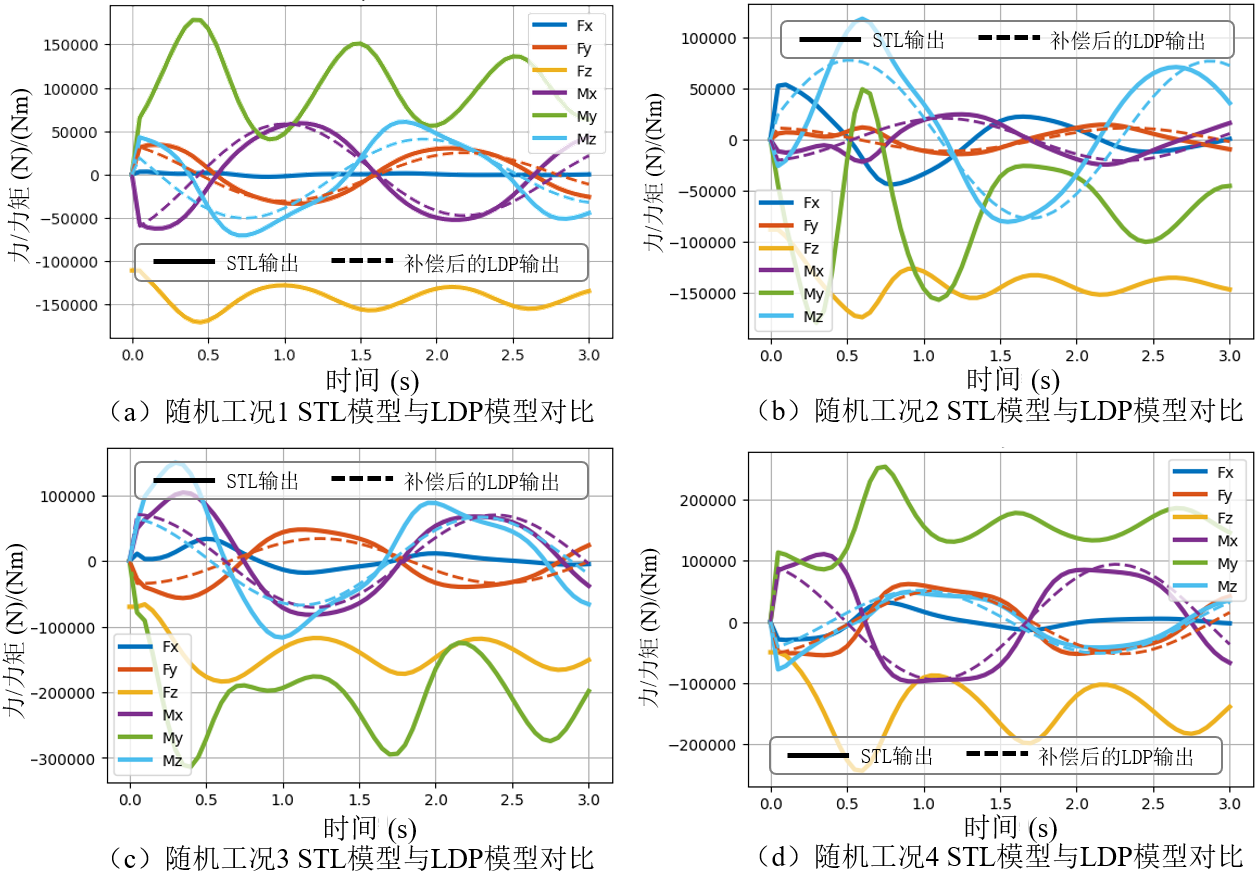
\includegraphics[width=1.0\linewidth]{fig/chap4/random_condition.png}
            \caption{随机工况下的重线性化模型\SI{3}{s}时域内拟合效果}
            \label{fig:random_condition}
            \end{figure}

            最后如图~\ref{fig:random_condition}所示为经过神经网络重线性化后的LDP模型在任意生成的工况下\SI{3}{s}预测时域内精准拟合CFD结果的示意，实现了线性模型在各个工况下都可以达到高精度的突破。在图~\ref{fig:ablation_test}中，进一步展示了残差模型消融测试的结果，即分别采用基础LDP、基础LDP+残差模型参数补偿、基础LDP+参数补偿与状态估计3种方案，对比了其在\SI{12}{s}的时间内对双移线工况下STL晃动的拟合效果。可以看出，最优参数的基础LDP模型在\SI{2}{s}内精度很高，但随时间推移误差累计逐渐发散；加入残差模型参数实时补偿后的模型进行递推则可得到收敛的结果，但细节仍然需要加强；当进一步加入状态实时估计后趋势与细节可以基本完全拟合，验证了残差模型的有效性。
            \begin{figure}
            \centering
            \subcaptionbox{在16工况下参数最优的基础LDP\label{fig:ga_raw}}
                {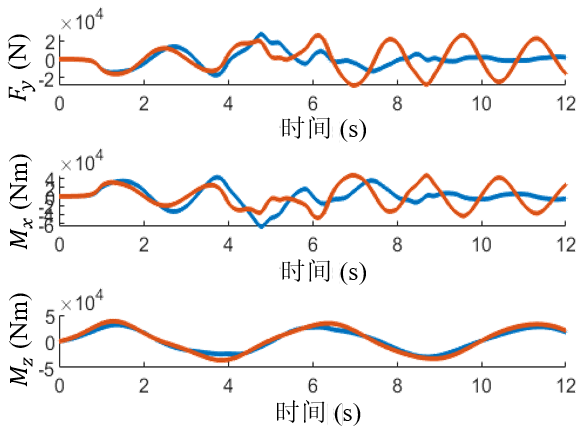
\includegraphics[width=0.48\linewidth]{fig/chap4/ga_raw.png}}
            \subcaptionbox{基础LDP+残差模型参数补偿 \label{fig:add_param}}
                {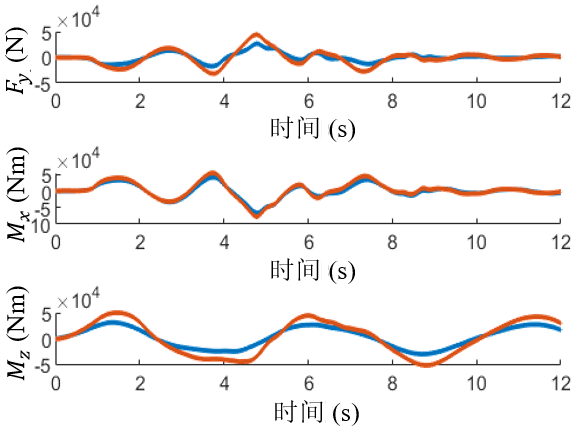
\includegraphics[width=0.48\linewidth]{fig/chap4/add_param.png}}
            \subcaptionbox{基础LDP+参数补偿与状态估计 \label{fig:add_all}}
                {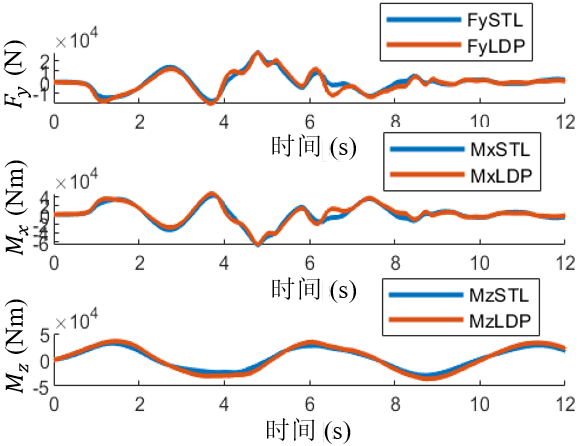
\includegraphics[width=0.48\linewidth]{fig/chap4/add_all.png}}
            \subcaptionbox{残差模型输出参数与状态估计 \label{fig:neural_out}}
                {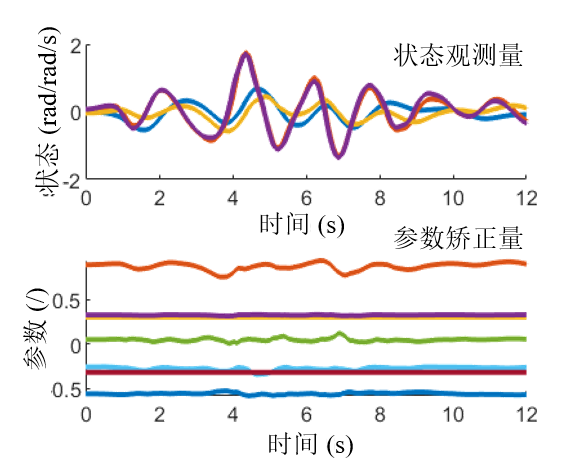
\includegraphics[width=0.48\linewidth]{fig/chap4/neural_out.png}}
            \caption{随机残差模型消融测试}
            \label{fig:ablation_test}
            \end{figure}

            借助残差模型，可以将LDP模型的参数与状态实时补偿，间接将STL模型在每个周期内线性化，实现了线性模型前提下对于液体晃动的高精度预测。
            

\section{轨迹跟踪抑晃防侧翻控制}
\label{sec:anti_rollover_tracking}
    \subsection{横纵向耦合半挂液罐车模型}
        \label{sub:lonlot_coupled_semi_trailer_model}
        本小节基于第\ref{subsub:ldp}节可以动态更新的罐液耦合模型建立液罐车车液耦合动力学模型。液罐车车液耦合动力学模型为2自由度的LDP与6自由度的半挂式液罐车模型（包含牵引车的4个自由度：纵移、侧滑、横摆、侧倾，以及挂车的2个自由度：横摆、侧倾）组成的8自由度模型。其中LDP为线性模型，由2个线性化单摆模型组成，包含2个摆动自由度，每个单摆模型都考虑侧倾角和侧向加速度两个输入。

        纵向运动采用简化表达，并主要通过参数标定实现。通过$v_{des}$的大小控制期望车速；为与实际变速特性匹配，控制量$v_{des}$与实际速度$v_x$之间的差值需设置阈值约束。由于实际加速度存在上限，可通过施加二者差值的方式模拟该特性，从而保证预测效果与实际效果之间的匹配性。此时需要在输出量中加入$v_x$的预测值；也可直接加入驱动加速度项$a_d$，再通过转换将其变为期望速度输入给下层控制器。

        \begin{figure}
        \centering
        \subcaptionbox{车身与罐体坐标系定义 \label{fig:coord_def}}
            {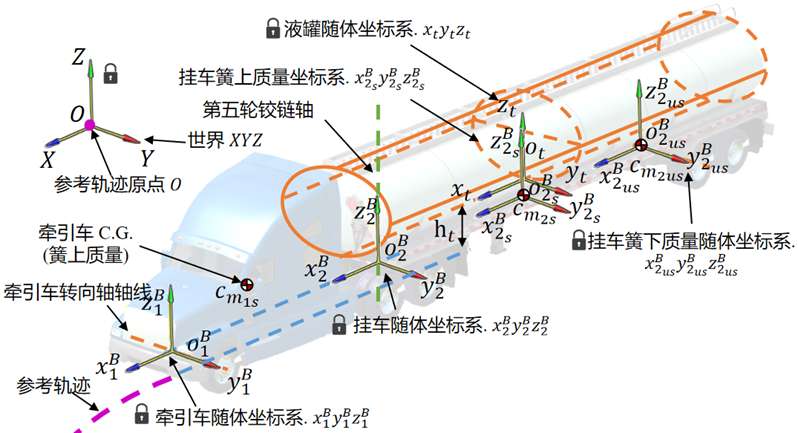
\includegraphics[width=0.68\linewidth]{fig/chap4/coord_def.png}}
        \subcaptionbox{侧倾平面内简化模型 \label{fig:trailer_model_lat}}
            {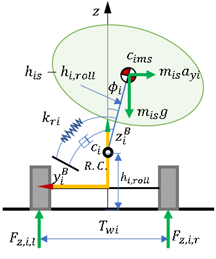
\includegraphics[width=0.3\linewidth]{fig/chap4/trailer_model_lat.png}}
        \subcaptionbox{横摆平面内简化模型 \label{fig:trailer_model_lon}}
            {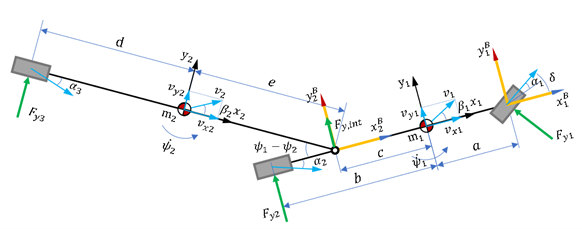
\includegraphics[width=1.0\linewidth]{fig/chap4/trailer_model_lon.png}}
        \caption{横纵向耦合半挂液罐车模型示意图}
        \label{fig:trailer_model_illust}
        \end{figure}


        \begin{equation}
        \begin{aligned}
        \dot{v}_x &= -c_{M1}(M_{1z}^+ + M_{1z}^-) - c_{M2}(M_{2z}^+ + M_{2z}^-) - F_{y1}\delta - \frac{1}{\tau_v}v_x + \frac{1}{\tau_v}v_{des} \\
        &= -c_{brk}\left(p_{brk}^{L1} + p_{brk}^{R1} + p_{brk}^{L2} + p_{brk}^{R2}\right) - \frac{1}{\tau_v}v_x + \frac{1}{\tau_v}v_{des}
        \end{aligned}
        \end{equation}

        施加一个约束：$v_{des} - v_x \leq \Delta v_{thrld}$

        令$c_{M1} = \frac{2}{T_{w1}(m_1 + m_2 + m_0 + m_p)} = 0.235e^{-4}$，$c_{M2} = \frac{2}{T_{w2}(m_1 + m_2 + m_0 + m_p)} = 0.24e^{-4}$（默认这些控制量$M_z$单位是\si{N m}）

        实际的给车辆下层控制器的期望速度指令为：$v_{des}^a = v_{des} + v_{dev}$，其中$v_{dev}$是静态偏置加速度，表达的是当期望速度等于实际速度时，实际速度会下降而非维持在期望速度的问题。即通常下层控制器特性满足期望速度比实际速度高且存在稳态误差的情况。

        关于制动压力与减速度之间的关系进行了如下标定，$a_{deccel} = c_{brk} \sum_{i=1}^N p_{brk}$。





        \begin{equation}
        \begin{aligned}
        a_{deccel} &= c_{brk} \sum_{i=1}^N p_{brk} \\
        &= c_{brk}\left(p_{brk}^{L1} + p_{brk}^{R1} + p_{brk}^{L2} + p_{brk}^{R2}\right) = c_{M1}(M_{1z}^+ + M_{1z}^-) + c_{M2}(M_{2z}^+ + M_{2z}^-)
        \end{aligned}
        \end{equation}

        $M_{1z}^+ \approx \frac{c_{brk}}{c_{M1}} p_{brk}^{L1} = \frac{0.62}{0.2375} p_{brk}^{L1} = 2.61 p_{brk}^{L1}$

        半挂车剩余5个自由度建模如图~\ref{fig:trailer_model_lat}和图~\ref{fig:trailer_model_lon}所示，参考宗长富\cite{zongchangfu2014identification}等的工作，牵引车侧滑、横摆、侧倾运动3个自由度建模为式\eqref{eq:tractor_lat}至式\eqref{eq:tractor_roll}。模型相关变量如表~\ref{tab:tank_truck_parameters}所示。



        {% 局部作用域，只改本表行距，不影响全文
        \small
        % \setlength{\tabcolsep}{3pt}       % 如需压缩列间距可取消注释
        \renewcommand{\arraystretch}{1.0} % 核心：恢复正常紧凑行距
        \linespread{0.7}\selectfont       % 强制行高

        \begin{longtable}{l l}
            \caption{简化半挂液罐车模型参数与变量说明}
            \label{tab:tank_truck_parameters} \\
            \toprule
            \textbf{参数/变量} & \textbf{说明（i=1,2 分别代表牵引车、挂车）} \\
            \midrule
        \endfirsthead
            \caption*{续表~\thetable\quad 简化半挂液罐车模型参数与变量说明} \\
            \toprule
            \textbf{参数/变量} & \textbf{说明（i=1,2 分别代表牵引车、挂车）} \\
            \midrule
        \endhead
            \bottomrule
        \endfoot

        %-------------------------------------------------------------------------------
        $m_i$, $m_{si}$ & 车辆总质量、簧载质量 \\
        $v_{ix}$, $v_{iy}$ & 纵向/侧向速度 \\
        $\dot{\beta_i}$ & 质心侧偏角变化率 \\
        $\psi_i$, $\phi_i$ & 横摆角、侧倾角 \\
        $\dot{\psi}_i$ & 横摆角速度 \\
        $\dot{\phi}_i$ & 侧倾角速度 \\
        $h_i$ & 质心到侧倾中心的距离 \\
        $h_{ic}$ & 牵引销到侧倾轴线的高度 \\
        $I_{izz}$, $I_{ixx}$, $I_{1xz}$ & 簧载质量在横摆、侧倾、交叉耦合方向的转动惯量 \\
        $k_{ri}$,$c_i$ & 悬架侧倾刚度/阻尼 \\
        $F_{y1}$, $F_{y2}$, $F_{y3}$ & 牵引车等效前轴、后轴，以及挂车等效后轴的侧向力 \\
        $F_z$ & 车轮所受垂向力 \\
        $F_{y,int}$ & 挂车作用于牵引车的侧向力 \\
        $F_x$, $F_y$, $M_x$, $M_y$, $M_z$ & 液体晃动纵向力、侧向力、侧倾力矩、俯仰力矩、横摆力矩 \\
        $a$, $b$, $c$ & 牵引车前轮轴/后轮轴/牵引销铰接点到质心的距离 \\
        $d$, $e$ & 挂车后轮轴/牵引销铰接点到质心的距离 \\
        $k_{12}$ & 牵引销连接部位的侧倾刚度 \\
        $k_1$, $k_2$, $k_3$ & 牵引车等效前轴、后轴，以及挂车后轴的侧向刚度 \\
        $\theta_1,\theta_2$ & 线性化双摆模型摆角 \\
        $\dot{\theta}_1,\dot{\theta}_2$ & 线性化双摆模型前/后摆角速度 \\
        $\delta$, $\delta_d$ & 转向角、期望转向角 \\
        $a_{deccel}$ & 车辆减速度 \\
        $c_{M1}$ & 牵引车制动力矩-减速度转换系数 \\
        $c_{M2}$ & 挂车制动力矩-减速度转换系数 \\
        $c_{brk}$ & 制动压力-减速度转换系数 \\
        $\tau_v$ & 车速响应时间常数 \\
        $v_{des}$ & 期望车速 \\
        $\Delta v_{thrld}$ & 期望车速与实际车速差值阈值 \\
        $v_{des}^a$ & 给下层控制器的期望速度指令 \\
        $v_{dev}$ & 静态偏置加速度 \\
        $p_{brk}^{L1}$ & 牵引车左侧制动压力 \\
        $p_{brk}^{R1}$ & 牵引车右侧制动压力 \\
        $p_{brk}^{L2}$ & 挂车左侧制动压力 \\
        $p_{brk}^{R2}$ & 挂车右侧制动压力 \\
        $M_{1z}^+$ & 牵引车左侧附加横摆力矩 \\
        $M_{1z}^-$ & 牵引车右侧附加横摆力矩 \\
        $M_{2z}^+$ & 挂车左侧附加横摆力矩 \\
        $M_{2z}^-$ & 挂车右侧附加横摆力矩 \\
        $T_{w1}$ & 牵引车轮距 \\
        $T_{w2}$ & 挂车轮距 \\
        $Y_1$ & 牵引车在大地坐标系下的Y轴坐标 \\
        $X_1$ & 牵引车在大地坐标系下的X轴坐标 \\
        \end{longtable}
        }% 结束局部作用域
        \begin{equation}
        m_1 v_{1x}(\dot{\beta}_1 + \dot{\psi}_1) - m_{1s} h_1 \ddot{\phi}_1 = F_{y1} + F_{y2} + F_{y,int}
        \label{eq:tractor_lat}
        \end{equation}
        \begin{equation}
        \begin{aligned}
        I_{1zz} \ddot{\psi}_1 - I_{1xz} \ddot{\phi}_1 &= F_{y1} a \cos \delta - F_{y2} b - F_{y,int} c + 10^4 \times (M_{1z}^+ - M_{1z}^-) \\
        &= F_{y1} a \cos \delta - F_{y2} b - F_{y,int} c + 10^4 \times \frac{c_{brk}}{\overline{c_M}} \left(p_{brk}^{L1} - p_{brk}^{R1}\right)
        \end{aligned}
        \label{eq:tractor_yaw}
        \end{equation}
        \begin{equation}
        \begin{aligned}
        &[I_{1xx} + m_{1s} h_1^2] \ddot{\phi}_1 - I_{1xz} \ddot{\psi}_1 = m_{1s} g h_1 \sin \phi_1 + m_{1s} h_1 \left[ v_{1x}(\dot{\beta}_1 + \dot{\psi}_1) - h_1 \ddot{\phi}_1 \right] \\
        &- k_{r1} \phi_1 - c_1 \dot{\phi}_1 + k_{12}(\phi_2 - \phi_1) - F_{y,int} h_{1c}
        \end{aligned}
        \label{eq:tractor_roll}
        \end{equation}
        半挂车侧滑、横摆、侧倾运动包含的2个自由度，分别为式\eqref{eq:trailer_lon}至式\eqref{eq:trailer_roll}。
        \begin{equation}
        m_2 v_{2x}(\dot{\beta}_2 + \dot{\psi}_2) - m_{2s} h_2 \ddot{\phi}_2 = F_{y3} - F_{y,int} \cos(\psi_1 - \psi_2) + F_{y,p1} + F_{y,p2}
        \label{eq:trailer_lon}
        \end{equation}
        \begin{equation}
        \begin{aligned}
        I_{2zz} \ddot{\psi}_2 - I_{2xz} \ddot{\phi}_2 &= -F_{y3} d - F_{y,int} e \cos(\psi_1 - \psi_2) + 10^4 \times (M_{2z}^+ - M_{2z}^-) + M_{2z,p} \\
        &= -F_{y3} d - F_{y,int} e \cos(\psi_1 - \psi_2) + 10^4 \times \frac{c_{brk}}{\overline{c_M}} \left(p_{brk}^{L2} - p_{brk}^{R2}\right) + M_{2z,p}
        \end{aligned}
        \label{eq:trailer_yaw}
        \end{equation}
        \begin{equation}
        \begin{aligned}
        &[I_{2xx} + m_{2s} h_2^2] \ddot{\phi}_2 - I_{2xz} \ddot{\psi}_2 = m_{2s} g h_2 \sin \phi_2 + m_{2s} h_2 \left[ v_{2x}(\dot{\beta}_2 + \dot{\psi}_2) - h_2 \ddot{\phi}_2 \right] \\
        &- k_{r2} \phi_2 - c_2 \dot{\phi}_2 - k_{12}(\phi_2 - \phi_1) + F_{y,int} h_{2c} + M_{x,p}
        \end{aligned}
        \label{eq:trailer_roll}
        \end{equation}
        牵引车和挂车的运动学约束方程如式\eqref{eq:trailer_constraint}描述。
        \begin{equation}
        \dot{\beta}_1 - \dot{\beta}_2 - \frac{h_{1c}}{v_{1x}} \ddot{\phi}_1 + \frac{h_{2c}}{v_{2x}} \ddot{\phi}_2 - \frac{c}{v_{1x}} \ddot{\psi}_1 - \frac{e}{v_{2x}} \ddot{\psi}_2 + \dot{\psi}_1 - \dot{\psi}_2 = 0
        \label{eq:trailer_constraint}
        \end{equation}
        由于采用线性轮胎模型，则各等效轴的侧向力可以近似为
        \begin{equation}
        \begin{cases}
        F_{y1} = k_1 \left( \beta_1 + \frac{a \dot{\psi}_1}{v_{1x}} - \delta \right) \\
        F_{y2} = k_2 \left( \beta_1 - \frac{b \dot{\psi}_1}{v_{1x}} \right) \\
        F_{y3} = k_3 \left( \beta_2 - \frac{d \dot{\psi}_1}{v_{2x}} \right)
        \end{cases}
        \end{equation}
        为实现对车辆动力学、摆模型计算，以及满足轨迹跟踪对车辆位姿状态量预测的需求，选取如下16个状态量构建状态空间方程，状态量分别为
        \begin{equation}
        X = \left[ v_{1y}\ \dot{\psi}_1\ \phi_1\ \dot{\phi}_1\ v_{2y}\ \dot{\psi}_2\ \phi_2\ \dot{\phi}_2\ \theta_1\ \dot{\theta}_1\ \theta_2\ \dot{\theta}_2\ v_{1x}\ \psi_1\ Y_1\ X_1 \right]^T
        \end{equation}
        \noindent 其中，$v_{1y}$为牵引车侧向速度、$\dot{\psi}_1$为牵引车航向角速度、$\phi_1$为牵引车侧倾角、$\dot{\phi}_1$为牵引车侧倾角速度、$v_{2y}$为挂车侧向速度、$\dot{\psi}_2$为挂车航向角速度、$\phi_2$为挂车侧倾角、$\dot{\phi}_2$为挂车侧倾角速度、$\theta_1$为双摆前摆角度、$\dot{\theta}_1$为双摆前摆角速度、$\theta_2$为双摆后摆角度、$\dot{\theta}_2$为双摆后摆角速度、$v_{1x}$为牵引车随车体坐标系下的纵向速度、$Y_1$为牵引车在大地坐标系下的Y轴坐标、$X_1$为牵引车在大地坐标系下的X轴坐标。由于纵向晃动对于加速的影响可以忽略，故不采用三摆模型，而是采用双摆模型。
        \begin{figure}
        \centering
        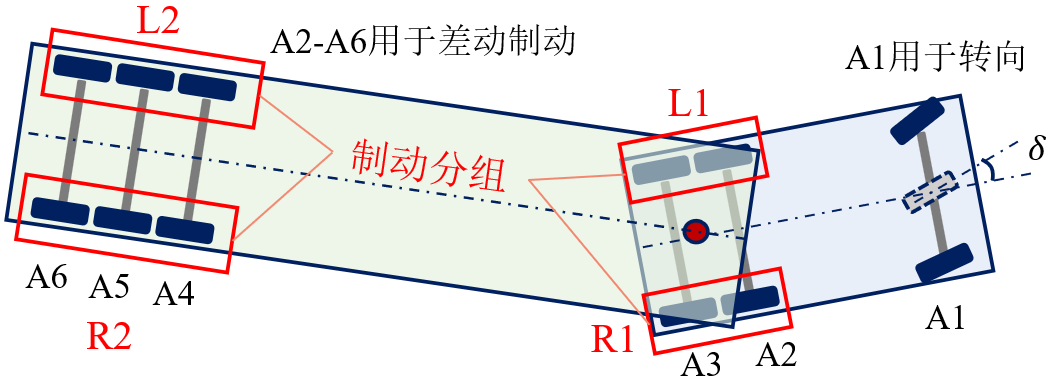
\includegraphics[width=0.6\linewidth]{fig/chap4/control_scheme.png}
        \caption{轨迹跟踪抑晃防侧翻控制方案}
        \label{fig:control_scheme}
        \end{figure}
        控制方案如图~\ref{fig:control_scheme}所示，第一轴完全负责转向控制，牵引车剩余轴、挂车所有轴负责差动制动控制。通过制动分组的方式将负责差动制动的车轮分为L1/L2/R1/R2共4组，组内制动行为完全相同。控制量为6部分：前轮转角、牵引车附加横摆力矩、挂车附加横摆力矩，以及牵引车的期望加速度。
        \begin{equation}
        u = \begin{bmatrix}
        \delta &
        p_{brk}^{L1} &
        p_{brk}^{R1} &
        p_{brk}^{L2} &
        p_{brk}^{R2} &
        v_{des}
        \end{bmatrix}^T
        \end{equation}

        线性化后的车辆状态空间方程建立如下：
        \begin{equation}
        \dot{X} = A_c X + B_c u, \quad
        A_c = T_c M^{-1} A_0 T_c^{-1} X,\quad B_c = T_c M^{-1} B_0
        \end{equation}
        \noindent 其中，$M$、$A_0$、$B_0$、$T_c$的详细展开见式\eqref{eq:M}、式\eqref{eq:A_0}、式\eqref{eq:B_0}、式\eqref{eq:T_c}。
        
        \setcounter{MaxMatrixCols}{20} % 至少 >= 16

        \begin{equation}
        M = \begin{bmatrix}
        m_{11} & I_{1zz} & 0 & m_{14} & 0 & 0 & 0 & 0 & 0 & 0 & 0 & 0 & 0 & 0 & 0 & 0 \\
        m_{21} & -I_{1xz} & 0 & m_{24} & 0 & 0 & 0 & 0 & 0 & 0 & 0 & 0 & 0 & 0 & 0 & 0 \\
        m_{31} & 0 & 0 & m_{34} & m_{35} & m_{36} & 0 & m_{38} & 0 & m_{310} & 0 & m_{310} & 0 & 0 & 0 & 0 \\
        0 & 0 & 0 & 0 & m_{45} & m_{46} & 0 & m_{48} & 0 & m_{410} & 0 & m_{412} & 0 & 0 & 0 & 0 \\
        0 & 0 & 0 & 0 & m_{55} & m_{56} & 0 & m_{58} & 0 & m_{510} & 0 & m_{510} & 0 & 0 & 0 & 0 \\
        1 & -\frac{c}{v_{1x}} & 0 & -\frac{h_{1c}}{v_{1x}} & -1 & -\frac{e}{v_{2x}} & 0 & \frac{h_{2c}}{v_{2x}} & 0 & 0 & 0 & 0 & 0 & 0 & 0 & 0 \\
        0 & 0 & 1 & 0 & 0 & 0 & 0 & 0 & 0 & 0 & 0 & 0 & 0 & 0 & 0 & 0 \\
        0 & 0 & 0 & 0 & 0 & 0 & 1 & 0 & 0 & 0 & 0 & 0 & 0 & 0 & 0 & 0 \\
        0 & 0 & 0 & 0 & 0 & 0 & 0 & 0 & 1 & 0 & 0 & 0 & 0 & 0 & 0 & 0 \\
        0 & 0 & 0 & 0 & \frac{v_{2x}}{l_p} & \frac{x_1}{l_p} & 0 & \frac{h_p}{l_p} & -2 & 0 & 1 & 0 & 0 & 0 & 0 & 0 \\
        0 & 0 & 0 & 0 & 0 & 0 & 0 & 0 & 0 & 0 & 0 & 1 & 0 & 0 & 0 & 0 \\
        0 & 0 & 0 & 0 & \frac{v_{2x}}{l_p} & \frac{x_2}{l_p} & 0 & \frac{h_p}{l_p} & -2 & 0 & 0 & 0 & 1 & 0 & 0 & 0 \\
        0 & 0 & 0 & 0 & 0 & 0 & 0 & 0 & 0 & 0 & 0 & 0 & 0 & 0 & 0 & 1 \\
        0 & 1 & 0 & 0 & 0 & 0 & 0 & 0 & 0 & 0 & 0 & 0 & 0 & 0 & 0 & 0
        \end{bmatrix}_{16 \times 16}
        \label{eq:M}
        \end{equation}
        \noindent 其中，各个子项为：
        \begin{equation*}
        \begin{aligned}
        m_{11} &= m_1 v_{1x} c, \quad
        m_{14} = -m_{1s} h_1 c - I_{1xz}, \quad
        m_{21} = (m_1 h_1 c - m_{1s} h_1) v_{1x}, \\
        m_{24} &= I_{1xx} + 2 m_{1s} h_1^2 - m_{1s} h_1 h_{1c}, \quad
        m_{31} = m_1 v_{1x}, \quad
        m_{34} = -m_{1s} h_1, \\
        m_{35} &= m_2 v_{2x} + (m_p + m_0) v_{2x}, \quad
        m_{36} = x_0 (m_p + m_0), \quad
        m_{38} = -m_{2s} h_2 - (m_0 h_0 + m_p h_p), \\
        m_{310} &= \frac{1}{2} m_p l_p, \quad
        m_{45} = e m_{35} - x_0 (m_p + m_0) v_{x2}, \quad
        m_{46} = -I_{2zz} + e m_{36} - \frac{1}{2} (m_p + m_0) (x_1^2 + x_2^2), \\
        m_{48} &= I_{2xz} + e m_{38} + x_0 (m_0 h_0 + m_p h_p), \quad
        m_{410} = e m_{310} - \frac{1}{2} m_p l_p x_1 = \frac{1}{2} (e - x_1) m_p l_p, \\
        m_{412} &= e m_{310} - \frac{1}{2} m_p l_p x_2 = \frac{1}{2} (e - x_2) m_p l_p, \\
        m_{55} &= (m_2 h_{2c} - m_{2s} h_2) v_{2x} + h_{2c} (m_p + m_0) v_{2x} - v_{x2} (m_0 h_0 + m_p h_p), \\
        m_{56} &= -I_{2xz} + h_{2c} m_{36} - x_0 (m_0 h_0 + m_p h_p), \quad
        m_{58} = I_{2xx} + 2 m_{2s} h_2^2 + h_{2c} m_{38} + (m_0 h_0^2 + m_p h_p^2), \\
        m_{510} &= h_{2c} m_{310} - \frac{1}{2} m_p h_p l_p = \frac{1}{2} (h_{2c} - h_p) m_p l_p.
        \end{aligned}
        \end{equation*}
        \begin{equation}
        A_0 = \begin{bmatrix}
        a_{11} & a_{12} & 0 & 0 & 0 & 0 & 0 & 0 & 0 & 0 & 0 & 0 & 0 & 0 & 0 & 0 \\
        a_{21} & a_{22} & a_{23} & 0 & 0 & 0 & k_{12} & 0 & 0 & 0 & 0 & 0 & 0 & 0 & 0 & 0 \\
        a_{31} & a_{32} & 0 & 0 & k_3 & a_{36} & 0 & 0 & 0 & 0 & 0 & 0 & 0 & 0 & 0 & 0 \\
        0 & 0 & 0 & 0 & a_{45} & a_{46} & 0 & 0 & 0 & 0 & 0 & 0 & 0 & 0 & 0 & 0 \\
        0 & 0 & 0 & 0 & a_{55} & a_{56} & a_{57} & -c_2 & a_{59} & 0 & a_{59} & 0 & 0 & 0 & 0 & 0 \\
        0 & -1 & 0 & 0 & 0 & 1 & 0 & 0 & 0 & 0 & 0 & 0 & 0 & 0 & 0 & 0 \\
        0 & 0 & 0 & 1 & 0 & 0 & 0 & 0 & 0 & 0 & 0 & 0 & 0 & 0 & 0 & 0 \\
        0 & 0 & 0 & 0 & 0 & 0 & 0 & 0 & 1 & 0 & 0 & 1 & 0 & 0 & 0 & 0 \\
        0 & 0 & 0 & 0 & 0 & 0 & 0 & 0 & 0 & 1 & 0 & 0 & 0 & 0 & 0 & 0 \\
        0 & 0 & 0 & 0 & -\frac{v_{2x}}{l_p} & -\frac{g}{l_p} & 0 & -\frac{g}{l_p} & -c_d & 0 & 0 & 0 & 0 & 0 & 0 & 0 \\
        0 & 0 & 0 & 0 & 0 & 0 & 0 & 0 & 0 & 0 & 0 & 1 & 0 & 0 & 0 & 0 \\
        0 & 0 & 0 & 0 & -\frac{v_{2x}}{l_p} & 0 & -\frac{g}{l_p} & 0 & -\frac{g}{l_p} & 0 & 0 & -c_d & 0 & 0 & 0 & 0 \\
        0 & 0 & 0 & 0 & 0 & 0 & 0 & 0 & 0 & 0 & 0 & 0 & 0 & 0 & -\frac{1}{\tau_v} & 0 \\
        0 & 1 & 0 & 0 & 0 & 0 & 0 & 0 & 0 & 0 & 0 & 0 & 0 & 0 & 0 & 0
        \end{bmatrix}
        \label{eq:A_0}
        \end{equation}
        \noindent 其中，各个子项为：
        \begin{equation*}
        \begin{aligned}
        a_{11} &= (a + c)k_1 + (c - b)k_2, \quad
        a_{12} = \frac{a(a + c)k_1 - b(c - b)k_2}{v_{1x}} - m_1 v_{1x} c, \\
        a_{21} &= k_1 h_{1c} + k_2 h_{1c}, \quad
        a_{22} = \frac{(a k_1 - b k_2) h_{1c}}{v_{1x}} + (m_{1s} h_1 - m_1 h_{1c}) v_{1x}, \\
        a_{23} &= m_{1s} g h_1 - k_{r1} - k_{12}, \quad
        a_{31} = k_1 + k_2, \quad
        a_{32} = \frac{a k_1 - b k_2}{v_{1x}} - m_1 v_{1x}, \\
        a_{36} &= -\frac{d k_3}{v_{2x}} - m_2 v_{2x} - (m_0 + m_p) v_{2x}, \quad
        a_{45} = (d + e)k_3, \\
        a_{46} &= -\frac{d(e + d)k_3}{v_{2x}} - m_2 v_{2x} e - e(m_0 + m_p) v_{2x} + x_0 (m_p + m_0) v_{2x}, \quad
        a_{55} = k_3 h_{2c} e, \\
        a_{56} &= -\frac{d k_3 h_{2c}}{v_{2x}} + (m_{2s} h_2 - m_2 h_{2c}) v_{2x} + (m_0 h_0 + m_p h_p) v_{2x} - h_{2c} (m_0 + m_p) v_{2x}, \\
        a_{57} &= m_{2s} g h_2 - k_{r2} - k_{12} + (m_0 h_0 + m_p h_p) g, \quad
        a_{59} = -\frac{1}{2} m_p l_p g.
        \end{aligned}
        \end{equation*}
        \begin{equation}
        T_c = diag([v_{1x}\ 1\ 1\ 1\ v_{2x}\ 1\ 1\ 1\ 1\ 1\ 1\ 1\ 1\ 1])_{14 \times 14}
        \label{eq:T_c}
        \end{equation}
        \begin{equation}
        B_0 = \begin{bmatrix}
        -(c + a)k_1 & \frac{c_{brk}}{\overline{c_M}} & -\frac{c_{brk}}{\overline{c_M}} & 0 & 0 & 0 \\
        -k_1 h_{1c} & 0 & 0 & 0 & 0 & 0 \\
        -k_1 & 0 & 0 & 0 & 0 & 0 \\
        0 & 0 & 0 & -\frac{c_{brk}}{\overline{c_M}} & \frac{c_{brk}}{\overline{c_M}} & 0 \\
        0 & 0 & 0 & 0 & 0 & 0 \\
        0 & 0 & 0 & 0 & 0 & 0 \\
        0 & 0 & 0 & 0 & 0 & 0 \\
        0 & 0 & 0 & 0 & 0 & 0 \\
        0 & 0 & 0 & 0 & 0 & 0 \\
        0 & 0 & 0 & 0 & 0 & 0 \\
        0 & 0 & 0 & 0 & 0 & 0 \\
        0 & 0 & 0 & 0 & 0 & 0 \\
        0 & -c_{brk} & -c_{brk} & -c_{brk} & -c_{brk} & \frac{1}{\tau_v} \\
        0 & 0 & 0 & 0 & 0 & 0
        \end{bmatrix}_{14 \times 6}
        \label{eq:B_0}
        \end{equation}



        
        
        求解时对状态空间方程进行零阶保持离散化（Zero Order Hold, ZOH），即

        \begin{equation}
        X(k) = A_d X(k - 1) + B_d \delta(k)
        \label{eq:discrete_state_space}
        \end{equation}

        \noindent 其中，$k$表示第$k$时刻，离散状态转移矩阵$A$与输入矩阵$B$采用如下方式获得：

        \begin{equation}
        \begin{bmatrix}
        A_d & B_d \\
        \mathbf{0}_{n_u \times n_x} & I_{n_u}
        \end{bmatrix} = \text{expm}\left( T_s \begin{bmatrix}
        A_c & B_c \\
        \mathbf{0}_{n_u \times n_x} & \mathbf{0}_{n_u}
        \end{bmatrix} \right)
        \end{equation}

        \noindent 其中，$T_s$为离散化模型的时间步长，$\text{expm}(\cdot)$为矩阵指数函数，$n_x$和$n_u$分别为模型的状态量个数和控制量个数，对于式\eqref{eq:discrete_state_space}分别为$n_x = 16$和$n_u = 6$。

        离散化状态转移矩阵$A$与输入矩阵$B$中$v_{1x}$与$v_{2x}$在计算时代入当前时刻的值，每个时刻重新计算矩阵$A$与$B$，形成线性时变模型。

        构建模型后，采用如第\ref{subsub:model_identification}节的方法利用遗传算法进行车辆参数识别，在TruckSim中构建前轮转角在第\SI{2}{s}阶跃的工况（阶跃动态符合二阶惯性系统）。其中利用拟合最优参数进行简化模型仿真中关键状态量的拟合结果如图~\ref{fig:state_fit}所示，在\SIrange{2}{8}{s}的时域内较好地拟合了TruckSim对应动力学仿真结果。

        \begin{figure}
        \centering
        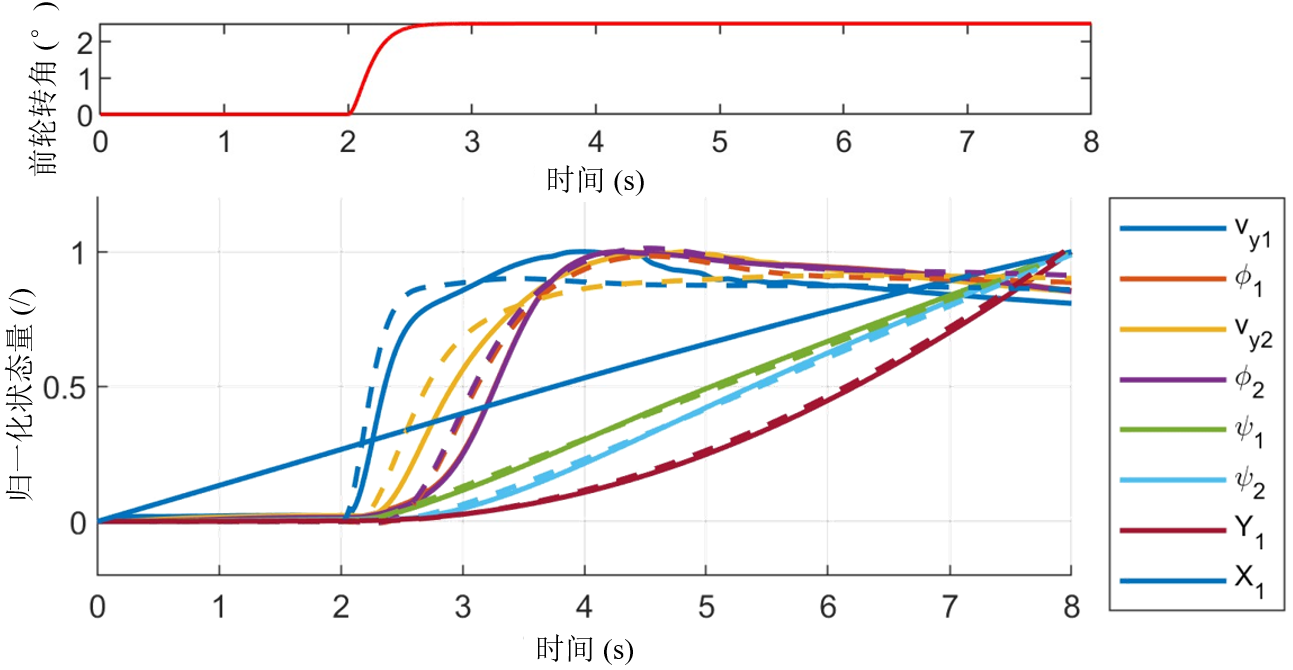
\includegraphics[width=0.8\linewidth]{fig/chap4/state_fit.png}
        \caption{前轮角阶跃工况车辆参数拟合后结果}
        \label{fig:state_fit}
        \end{figure}
      

    \subsection{多约束模型预测控制}
        \label{sub:multi_constraint_mpc}
        \setcounter{MaxMatrixCols}{20} % 至少 >= 16
        本节建立基于车辆状态来控制车轮转角（或车轮转角和驱/制动力）的基础控制器。基础控制器采用线性模型预测控制，预测时域至少大于1.5倍罐内液体横向晃动周期，且可以输出所采取的最优控制下的预测轨迹。

        \subsubsection{防侧翻轨迹跟踪控制策略设计}
            \label{subsub:anti_rollover_mechanism}
            采用多约束模型预测控制（multi-constraint model predictive control, MPC）方法，防侧翻路径跟踪能够显式考虑输入与输出约束。这保证了在模型精度合理的前提下，只要存在可行的控制解，车辆既不会发生侧翻，也不会违反其他可行性约束。当不存在满足所有约束的可行解时，求解器会在松弛因子的辅助下，优先违反最不关键的软约束，直至找到惩罚程度最低的可行解。

            \begin{figure}
            \centering
            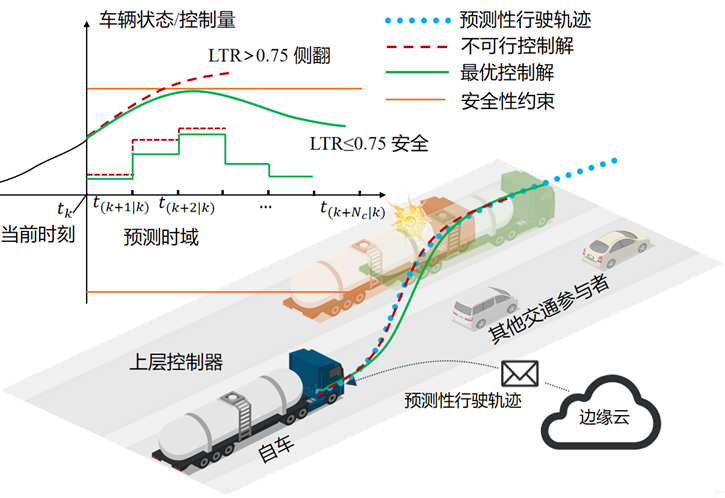
\includegraphics[width=0.7\linewidth]{fig/chap4/mpc_illust.png}
            \caption{防侧翻轨迹跟踪MPC控制示意图}
            \label{fig:mpc_illust}
            \end{figure}

            如图~\ref{fig:mpc_illust}所示，假设全局参考路径已通过基于云的预测性变道或其他路径规划应用获取，路径跟踪控制器将求解一个二次规划MPC问题，以得到能最小化软约束违反程度的可行控制序列，并选取首个控制输入作为实际控制输入。



            尽管横向误差是跟踪控制中广泛使用的状态变量\cite{Reviewer1_FuzzySteering}，可实现如图~\ref{fig:linear_tracker}所示的线性跟踪，但本研究采用绝对位置 \(Y_1, X_1\) 作为状态变量，以构建绝对跟踪器\cite{ShengboEbenLi2024reinforcement}，从而更精确地预测跟踪过程中的高阶动力学，如图~\ref{fig:absolute_tracker}所示。同时，通过将预测时域延长至1.5~3 s（覆盖约1 s的液体晃动周期\cite{Komasa2023observing}），可捕捉LTR动力学中的潜在间隙，提升MPC的有效性，相比简化动力学的线性跟踪器，能更好地保证车辆稳定性与安全性。

            \begin{figure}
            \centering
            \subcaptionbox{线性跟踪（$l_s \to 0$为切线跟踪）\label{fig:linear_tracker}}
                {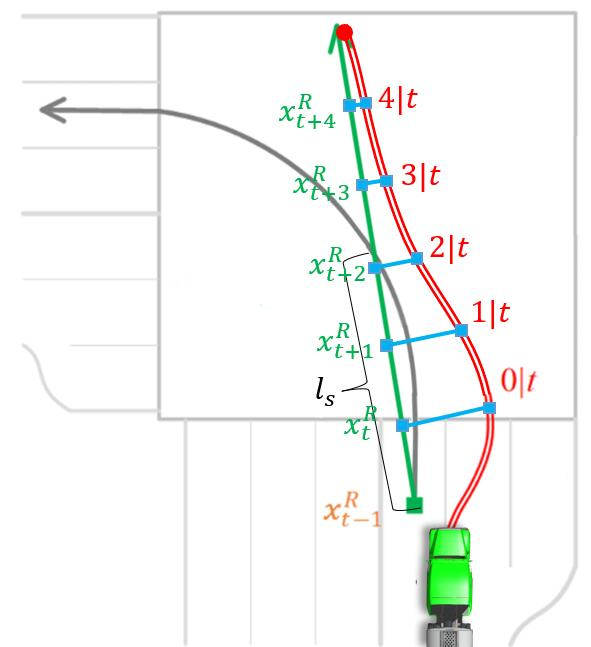
\includegraphics[width=0.40\linewidth]{fig/chap4/linear_tracker.jpg}}
            \subcaptionbox{绝对位置跟踪 \label{fig:absolute_tracker}}
                {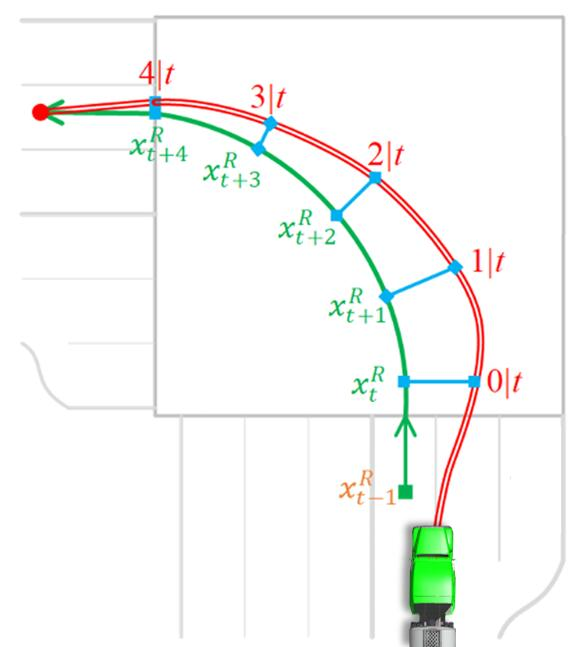
\includegraphics[width=0.40\linewidth]{fig/chap4/absolute_tracker.jpg}}
            \caption{线性跟踪与绝对位置跟踪方法对比}
            \label{fig:tracker_comparison}
            \end{figure}

            最优控制问题的构建过程包括观测量设计、代价函数构造、以及约束设计。观测量的设计如下：
            \begin{equation}
            y = [Y_1\ X_1\ \psi_1\ \dot{\theta}_1\ \dot{\theta}_2\ \mathrm{LTR}_{eql}\ v_{x1}]
            \end{equation}
            \noindent 其中，状态量可以按照作用分为三个部分：
            (1) 轨迹跟踪所用的车辆姿态$\psi_1$（减去了控制开始时刻的偏移量，这样可以避免角度超过限度后重新计算的问题）；
            (2) 正常行驶时抑晃所用的液体等效线性双摆的摆动角速度$\dot{\theta}_1\ \dot{\theta}_2$（由于摆动系统的相图近似呈环形，约束角速度这一坐标轴即可在较大程度上限制摆角）；
            (3) 极端工况防侧翻所用的基于悬架力等效载荷转移率$\mathrm{LTR}_{eql}$。

            一般采用悬架力等效的$\mathrm{LTR}_{eql}$作为替代：
            \begin{equation}
            \mathrm{LTR}_{eql} = c_r(-k_{r1}\phi_1 - c_1 \dot{\phi}_1 - k_{r2}\phi_2 - c_2 \dot{\phi}_2)
            \end{equation}
            \noindent 其中，系数$c_r$为：
            \begin{equation}
            c_r = \frac{2}{\frac{T_{w1} + T_{w2}}{2}(m_1 + m_2)g}
            \end{equation}

            $\mathrm{LTR}_{eql} \Leftrightarrow \mathrm{LTR}$的条件是：
            (1) $k_{r1}$、$k_{r2}$、$c_1$、$c_2$等悬架相关参数以及质量参数$m_1$、$m_2$、轮距$T_{w1}$、$T_{w2}$测量、识别与实际相应参数完全一致；
            (2) 车辆侧倾角$\phi_1$及侧倾角速度$\dot{\phi}_1$测量或估计结果与实际完全一致。

            实际应用中，上述两项条件难以完全满足，但仍然可以以较高精度获得$\mathrm{LTR}$的等效值。且由于$\mathrm{LTR}_{eql}$不存在$\pm1$饱和的问题，在一侧车轮离地后、接近侧翻但尚未真正侧翻的极危工况下，仍然可以准确反映车辆侧翻动态，且参数便于获取、易于计算。为实现上述输出量的观测，观测矩阵$C_d$应为
            \begin{equation}
            C_d = \begin{bmatrix}
            0 & 0 & 0 & 0 & 0 & 0 & 0 & 0 & 0 & 0 & 0 & 0 & 0 & 1 & 0 \\
            0 & 0 & 0 & 0 & 0 & 0 & 0 & 0 & 0 & 0 & 0 & 0 & 0 & 0 & 1 \\
            0 & 0 & 0 & 0 & 0 & 0 & 0 & 0 & 0 & 0 & 0 & 0 & 1 & 0 & 0 \\
            0 & 0 & 0 & 0 & 0 & 0 & 0 & 0 & 0 & 1 & 0 & 0 & 0 & 0 & 0 \\
            0 & 0 & 0 & 0 & 0 & 0 & 0 & 0 & 0 & 0 & 1 & 0 & 0 & 0 & 0 \\
            0 & 0 & -c_r k_{r1} & -c_r c_1 & 0 & 0 & -c_r k_{r2} & -c_r c_2 & 0 & 0 & 0 & 0 & 0 & 0 & 0 \\
            0 & 0 & 0 & 0 & 0 & 0 & 0 & 0 & 0 & 0 & 0 & 0 & 1 & 0 & 0
            \end{bmatrix}
            \end{equation}
            控制器对应三项功能：路径跟踪、液体晃动抑制与防侧翻。在路径跟踪环节，仅采用牵引车的状态变量，这是因为挂车轨迹会紧密跟随牵引车轨迹，从而简化传感器布置与计算复杂度。
        
        \subsubsection{最优化控制问题构建}
            \label{subsub:opt_prob_construct}
            所构建的离散时间模型为：
            \begin{equation}
            \begin{cases}
            x_{k+1} = A_d x_k + B_d u_k \\
            y_k = C_d x_k
            \end{cases}
            \end{equation}
            在此基础上为限制控制量增量，采用增量式MPC，构建新的状态量\cite{gongjianwei2020mpcbook}
            \begin{equation}
            \xi_k = \begin{bmatrix} x_k \\ u_{k-1} \end{bmatrix}
            \end{equation}
            那么新的状态空间表达式为
            \begin{equation}
            \xi_{k+1} = \begin{bmatrix} x_{k+1} \\ u_k \end{bmatrix} = \begin{bmatrix} A_d & B_d \\ 0 & I_{N_u} \end{bmatrix} \begin{bmatrix} x_k \\ u_{k-1} \end{bmatrix} + \begin{bmatrix} B_d \\ I_{N_u} \end{bmatrix} \Delta u_k \\
            = A \xi_k + B \Delta u_k
            \end{equation}
            \noindent 其中，$N_y$为输出量个数，输出方程为：
            \begin{equation}
            \eta_k = [C_d\ 0] \begin{bmatrix} x_k \\ u_{k-1} \end{bmatrix} = C \xi_k
            \end{equation}
            定义系统输出量的参考值
            \begin{equation}
            Y_r = [\eta_{r,k+1}^T\ \eta_{r,k+2}^T\ \cdots\ \eta_{r,k+N_p}^T]^T
            \end{equation}

            参考输出量的分量展开形式在本研究中为
            \begin{equation}
            \eta_{r,i} = [\theta_{r,i}\ \dot{\theta}_{r,i}\ \psi_{1,r,i}\ Y_{1,r,i}\ X_{1,r,i}\ \mathrm{LTR}_{eql,r,i}\ \delta_{r,i}]^T
            \end{equation}
            \begin{equation}
            Y = \begin{bmatrix} \eta_{k+1} \\ \eta_{k+2} \\ \vdots \\ \eta_{k+N_p} \end{bmatrix}, \Psi = \begin{bmatrix} C A \\ C A^2 \\ \vdots \\ C A^{N_p} \end{bmatrix}, \Delta U = \begin{bmatrix} \Delta u_k \\ \Delta u_{k+1} \\ \vdots \\ \Delta u_{k+N_c - 1} \end{bmatrix}
            \end{equation}
            \begin{equation}
            \Theta = \begin{bmatrix}
            C B & 0 & \cdots & 0 \\
            C A B & C B & 0 & \cdots & 0 \\
            \vdots & \vdots & \ddots & \vdots \\
            C A^{N_p - 1} B & C A^{N_p - 2} B & C A^{N_p - 3} B & \cdots & C B
            \end{bmatrix} T
            \end{equation}
            \begin{equation}
            T = \begin{bmatrix}
            1 & 0 & \cdots & 0 \\
            0 & q_{q1 \times 1} & 0 & \cdots & 0 \\
            \vdots & \vdots & \ddots & \vdots \\
            0 & 0 & \cdots & q_{qN_c - 1 \times 1}
            \end{bmatrix} \otimes I_{N_u}
            \end{equation}
            \begin{equation}
            \Pi = \begin{bmatrix}
            1 & 0 & \cdots & 0 \\
            0 & \pi_{1 \times p_1} & \cdots & 0 \\
            \vdots & \vdots & \ddots & \vdots \\
            0 & 0 & \cdots & \pi_{1 \times p_{N_r - 1}}
            \end{bmatrix} \otimes I_{N_y} \rightarrow \otimes [0\ 0\ 0\ 0\ 0\ 1\ 0\ 0]
            \end{equation}
            那么输出方程可以改写为
            \begin{equation}
            Y = \Psi \xi_k + \Theta \Delta U
            \end{equation}
            \noindent 其中，$T$和$\Pi$是为了加快运算速度而定义的压缩映射矩阵，子向量$q = [1\ 0]^T$，$\pi = [1\ 0]$，$N_c$和$N_r$分别为决策变量和约束时域个数，$N_c, N_r \leq N_p$。数列$\{q_1, q_2, \dots, q_{N_c - 1}\}$和$\{p_1, p_2, \dots, p_{N_r - 1}\}$任意元素大于等于1，且通常是递增。通过更多地减少预测时域内距当前时刻较远时刻的决策变量和输出量约束来极大减小二次规划的峰值求解时间，同时仅对控制量解的最优性产生小于\SI{1}{\percent}的影响\cite{shengbo2015fastmpc}。这对于状态维数较多的半挂液罐车的实时控制来说是必要的措施。

            令
            \begin{equation}
            E = \Psi \xi_k,\ Q_Q = I_{N_p} \otimes Q,\ R_R = I_{N_p} \otimes R
            \end{equation}
            \noindent 其中，$Q \in S_{++}^{N_y}$，$R \in S_+^{N_u}$，$\otimes$表示克罗内克积。

            定义代价函数为
            \begin{equation}
            \begin{aligned}
            J &= \tilde{Y}^T Q_Q \tilde{Y} + \Delta U^T R_R \Delta U \\
            &= (Y - Y_r)^T Q_Q (Y - Y_r) + \Delta U^T R_R \Delta U \\
            &= [(\Psi \xi_k + \Theta \Delta U) - Y_r]^T Q_Q [(\Psi \xi_k + \Theta \Delta U) - Y_r] + \Delta U^T R_R \Delta U \\
            &= [(E + \Theta \Delta U) - Y_r]^T Q_Q [(E + \Theta \Delta U) - Y_r] + \Delta U^T R_R \Delta U \\
            &= \Delta U^T (\Theta^T Q_Q \Theta + R_R) \Delta U + 2(E^T Q_Q \Theta - Y_r^T Q_Q \Theta) \Delta U + Const
            \end{aligned}
            \end{equation}
            令$H = (\Theta^T Q_Q \Theta + R_R)$，$g = (E^T Q_Q \Theta - Y_r^T Q_Q \Theta)^T$。对控制量和其增量施加范围约束
            \begin{equation}
            U = \begin{bmatrix}
            u_k \\ u_{k+1} \\ u_{k+2} \\ \vdots \\ u_{k+N_c - 1}
            \end{bmatrix} = \begin{bmatrix}
            u_{k-1} \\ u_{k-1} \\ u_{k-1} \\ \vdots \\ u_{k-1}
            \end{bmatrix} + \begin{bmatrix}
            I_{N_u} & 0 & 0 & \cdots & 0 \\
            I_{N_u} & I_{N_u} & 0 & \cdots & 0 \\
            I_{N_u} & I_{N_u} & I_{N_u} & \cdots & 0 \\
            \vdots & \vdots & \vdots & \ddots & 0 \\
            I_{N_u} & I_{N_u} & I_{N_u} & \cdots & I_{N_u}
            \end{bmatrix} \begin{bmatrix}
            \Delta u_k \\ \Delta u_{k+1} \\ \Delta u_{k+2} \\ \vdots \\ \Delta u_{k+N_c - 1}
            \end{bmatrix} = U_t + A_t \Delta U
            \end{equation}

            则对于控制量$U$的约束问题可以转化为对控制增量$\Delta U$的线性不等式约束
            \begin{equation}
            U_{min} = \begin{bmatrix}
            u_{min} \\ u_{min} \\ u_{min} \\ \vdots \\ u_{min}
            \end{bmatrix} \leq \begin{bmatrix}
            u_k \\ u_{k+1} \\ u_{k+2} \\ \vdots \\ u_{k+N_c - 1}
            \end{bmatrix} \leq \begin{bmatrix}
            u_{max} \\ u_{max} \\ u_{max} \\ \vdots \\ u_{max}
            \end{bmatrix} = U_{max} \\
            \Leftrightarrow \begin{cases}
            A_t \Delta U \leq U_{max} - U_t \\
            -A_t \Delta U \leq U_{min} + U_t
            \end{cases}
            \end{equation}
            同时，可直接对待优化的控制增量$\Delta U$施加范围约束
            \begin{equation}
            \Delta U_{min} \leq \Delta U \leq \Delta U_{max}
            \end{equation}
            对输出量的约束同样需要转化为对控制增量的约束。

            \begin{equation}
            Y_{min} - E \leq \Theta \Delta U \leq Y_{max} - E
            \end{equation}
            为对输出量施加软约束，避免同时对输入和输出施加硬约束导致约束相互冲突从而无解的情况出现，需要在代价函数$J$中引入松弛项$\rho \epsilon^2$，其中$\epsilon$为松弛因子，$\rho$为松弛系数。约束转变为
            \begin{equation}
            \begin{cases}
            \Theta \Delta U - \epsilon \leq Y_{max} - E \\
            -\Theta \Delta U - \epsilon \leq Y_{min} - E
            \end{cases}
            \end{equation}
            定义对控制变量$v_{des}$的约束为：
            $W = I_{N_p} \otimes w$
            \noindent 其中，$w = [0\ 0\ 0\ 0\ 0\ 0\ 1]$用于提取出$v_x$。
            \begin{equation}
            \begin{aligned}
            v_{des} &\leq v_{1x} + \Delta v_{thrld,1} \\
            v_{des} &\leq v_{1x} - \Delta v_{thrld,2} \\
            W_{N_p \times (N_y \times N_p)} Y &= W_{N_p \times (N_y \times N_p)} E + W_{N_p \times (N_y \times N_p)} \Theta \Delta U \\
            &\leq W_{N_p \times (N_y \times N_p)} A_t (N_u \times N_c) \times \Delta U (N_u \times N_c) \times 1
            \end{aligned}
            \end{equation}
            则MPC问题转化为标准二次型规划问题如下：
            \begin{equation}
            \underset{\Delta U}{\arg\min} J = \frac{1}{2} [\Delta U^T\ \epsilon] \begin{bmatrix} H & 0 \\ 0 & \rho \end{bmatrix} \begin{bmatrix} \Delta U \\ \epsilon \end{bmatrix} + [g^T\ 0] \begin{bmatrix} \Delta U \\ \epsilon \end{bmatrix}
            \end{equation}
            \begin{equation*}
            s.t.\quad
            \begin{cases}
            A_t \Delta U \leq U_{max} - U_t \\
            -A_t \Delta U \leq U_{min} + U_t \\
            \Pi \Theta \Delta U - \epsilon \leq \Pi (Y_{max} - E) \\
            -\Pi \Theta \Delta U - \epsilon \leq \Pi (Y_{min} - E) \\
            \Delta U_{min} \leq \Delta U \leq \Delta U_{max} \\
            \epsilon_{min} \leq \epsilon \leq \epsilon_{max}
            \end{cases}
            \end{equation*}
            代价函数构建完毕，这是一个标准二次型问题，可以通过OSQP、qpOASES、CVXOPT等二次规划求解器进行快速求解。本研究中选用qpOASES进行二次规划问题的求解。为了保证优化时变量的一致性，对输入量先进行归一化后再进行计算。为对行驶中可能的模型误差进行补偿，本节方法在实际部署中进行了无模型自适应滑模残差补偿\cite{KomasaQi2026MasterThesis_repo}。

            本章设计的控制算法用于自动驾驶半挂液罐车，但面向辅助驾驶环境仍然可通过控制器嵌套方法与人类驾驶员进行组合\cite{KomasaQi2026MasterThesis_repo}。

\section{仿真与缩比例模型试验设计与验证}
\label{sec:simulation_and_experiment}
    本节通过车液耦合联合仿真及缩比例模型车试验对防侧翻控制方法进行验证。首先，\ref{sub:cosim_platform}节建立了车液耦合联合仿真平台；其次，\ref{sub:simulation_verification}节利用建立的联合仿真平台对第\ref{sub:multi_constraint_mpc}节的防侧翻控制方法在典型危险工况下进行验证；最后，\ref{sub:model_truck_platform}节搭建了缩比例模型车平台，\ref{sub:model_experiment}节对简化的\ref{sub:multi_constraint_mpc}节方法进行了验证。

    \subsection{车液耦合联合仿真平台建立}
        \label{sub:cosim_platform}
        为了更好地验证所提出的防侧翻路径跟踪控制方法的有效性，本研究构建了如图~\ref{fig:cosim_arch}所示的车辆-流体耦合协同仿真平台。采用有限体积法（Finite Volume Method, FVM）对流体进行精确建模，基于CFD方法。设计了MATLAB函数与Java宏，以实现Simulink与StarCCM+之间的数据交互。创建了两个标志文件和两个数据交换文件，用于参数级交互，如图~\ref{fig:cosim_arch}所示。在每个时间步长内，TruckSim在StarCCM+中提供半挂车的加速度与角速度，通过改变重力模型分量与用户自定义体积力（详见表~\ref{tab:co_sim_settings}）作用于流体。同时，StarCCM+提供流体作用于罐体的三维力与力矩，再施加到TruckSim的半挂车模型中。该协同仿真方法实现了车辆动力学与CFD之间的实时（仿真中）交互，并在Simulink中搭建了联合仿真模型\cite{KomasaQi2026MasterThesis_repo}，包含StarCCM+的CFD仿真通信模块、与TruckSim通信的车辆模型、液体晃动观测用无迹卡尔曼滤波（Unscented Kalman Filter, UKF）与STL模型\cite{Komasa2023observing}、用于简化液体晃动的DLP模型、MPC+MFASMC组合控制器等。
        
        \begin{figure}
        \centering
        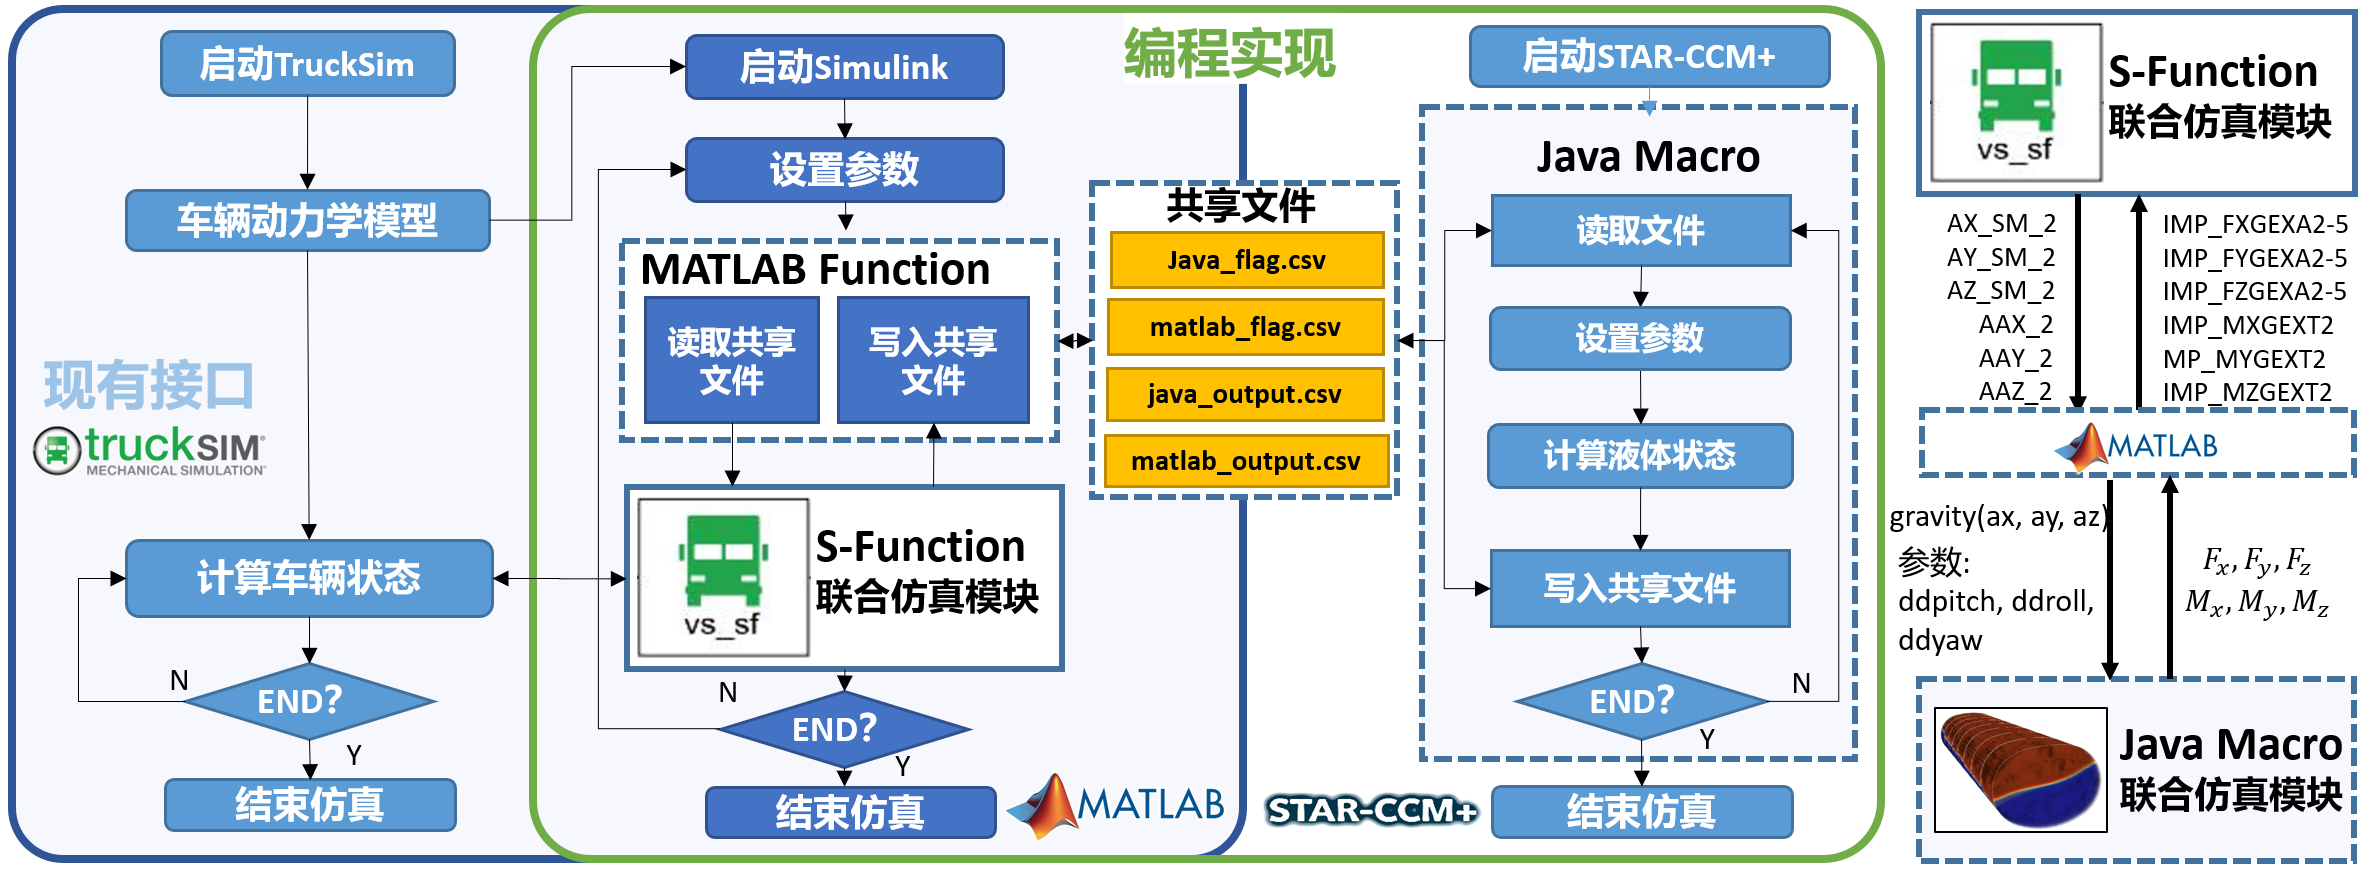
\includegraphics[width=1.0\linewidth]{fig/chap4/cosim_arch.png}
        \caption{车液耦合协同仿真平台架构}
        \label{fig:cosim_arch}
        \end{figure}



        在计算流体力学仿真中，网格尺寸越小，仿真结果往往越精确；但受计算机数值精度限制，并非网格尺寸越小越好，且过小的网格尺寸会带来急剧增长的网格数量，使得计算时间变得难以接受。为在保证仿真准确性的同时兼顾高效性，本文开展了如图~\ref{fig:grid_sensitivity}所示的网格敏感性分析。为建立参考结果，选取在特定设置下将单元加速度与角加速度施加于液体时能够达到最高精度的网格划分方式进行仿真（图~\ref{fig:grid_sensitivity_set}，左侧）。对比了六种替代设置，其仿真力/力矩相对误差结果如图~\ref{fig:grid_sensitivity_res}所示，图~\ref{fig:grid_sensitivity_set}展示了协同仿真中真实值对应的网格设置与所采用模型的网格设置；同时列出了网格敏感性验证中X/Y/Z方向的力（$F_x, F_y, F_z$）与X/Y/Z方向的力矩（$M_x, M_y, M_z$）的误差及时间平均误差。其中，$\text{rf}$为网格细化等级（refinement level），$b$为网格基础尺寸（base size of mesh），$\text{tw}$为过渡宽度（transition width），$\text{vi}$为体积增长速率（volume growth rate）；$\text{s}$和$\text{f}$分别为“慢（slow）”和“快（fast）”的缩写。所选设置（图~\ref{fig:grid_sensitivity_set}，右侧，蓝色曲线）实现了平均相对误差小于\SI{1}{\percent}、峰值误差低于\SI{4}{\percent}的效果。更多设置细节详见表~\ref{tab:co_sim_settings}。协同仿真所使用的计算机为13代Intel® Core™ i9-13900HX 2.20GHz处理器，配备32GB内存。



        \begin{figure}
        \centering
        \subcaptionbox{网格敏感性分析设置 \label{fig:grid_sensitivity_set}}
            {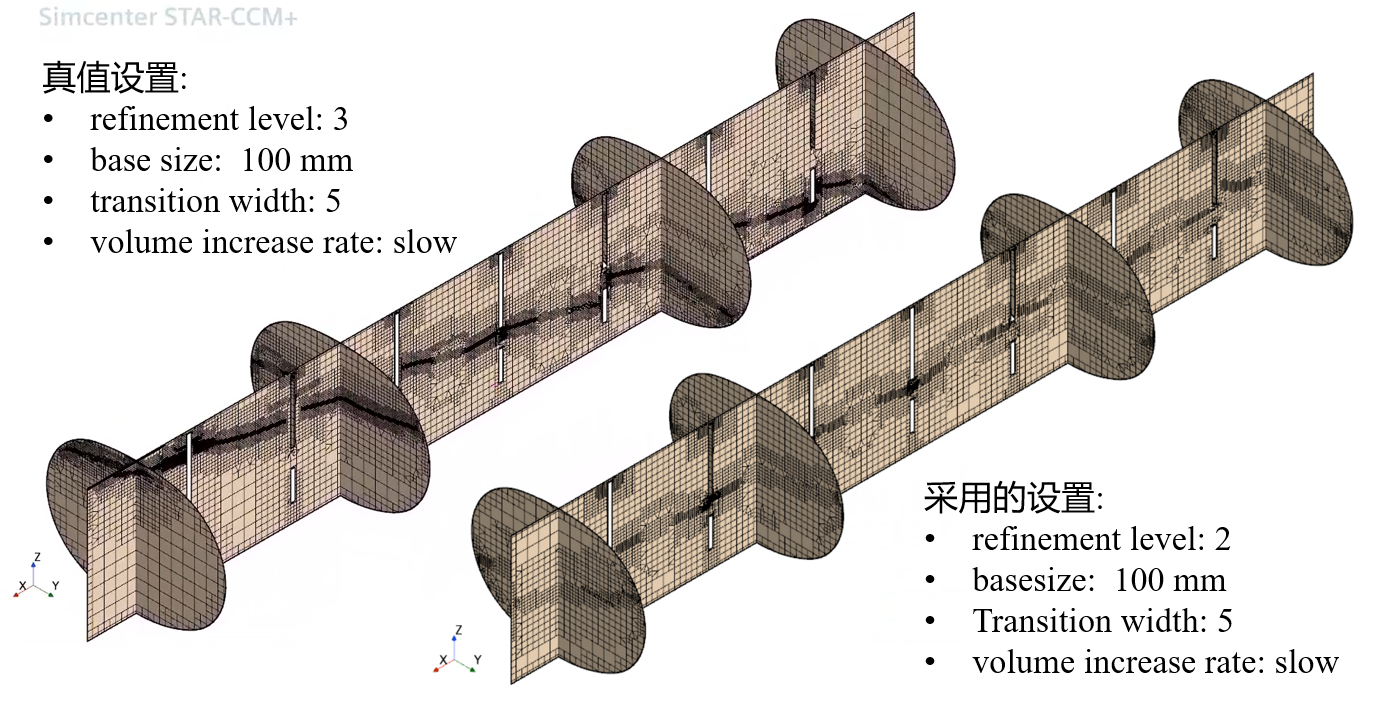
\includegraphics[width=0.8\linewidth]{fig/chap4/grid_sensitivity_set.png}}
        \subcaptionbox{网格敏感性分析结果 \label{fig:grid_sensitivity_res}}
            {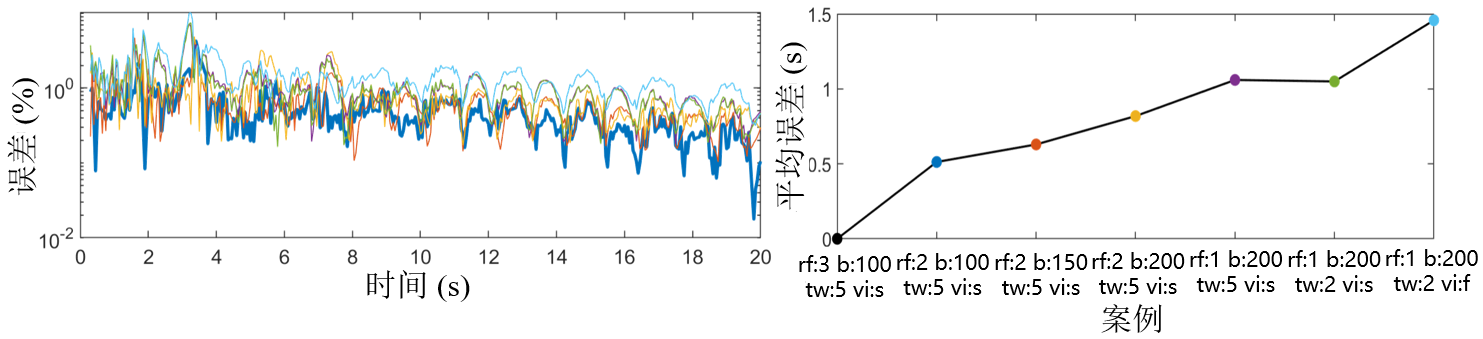
\includegraphics[width=1.0\linewidth]{fig/chap4/grid_sensitivity_res.png}}
        \caption{网格敏感性分析}
        \label{fig:grid_sensitivity}
        \end{figure}

        \begin{table}[htbp]
        \centering
        \small
        \linespread{0.8}\selectfont       % 强制行高
        \caption{协同仿真设置}
        \label{tab:co_sim_settings}
        \begin{tabularx}{\linewidth}{lX}
            \toprule
            项目 & 设置 \\
            \midrule
            软件配置 & Matlab R2023a、StarCCM+ 16.06.008-R8、TruckSim 2019.0 \\
            时间步长 & TruckSim：\SI{0.001}{s}；StarCCM+：自适应（\SIrange{1e-4}{0.005}{s}）；数据交换：\SI{0.005}{s} \\
            维度 & 三维 \\
            欧拉相 & $C_8H_{17}$（汽油）与空气，填充率\SI{50}{\percent} \\
            流型 & 分离流 \\
            湍流模型 & 可实现的k-ε两层模型 \\
            自适应时间步 & 时间提供器：自由面CFL条件 \\
            体网格 & 自适应自由面网格细化等级：2；基础尺寸：\SI{100}{mm}；过渡宽度：5；体积增长速率：慢 \\
            重力 & 通过Java宏在每个时间步修改 \\
            用户自定义函数 & \(\$\text{Density}*(\$\text{Position[2]}*\$\text{ddpitch}+\$\text{Position[1]}*\$\text{ddyaw}),\) \\
            & \((\$\text{Position[2]}*\$\text{ddroll}+\$\text{Position[0]}*\$\text{ddyaw}),\) \\
            & \((\$\text{Position[0]}*\$\text{ddpitch}+\$\text{Position[1]}*\$\text{ddroll})\) \\
            MPC设置 & 控制器频率：\SI{20}{Hz}；预测时域\(N_p = 40\)；控制步长\(N_c = 3\)；约束步长\(N_r = 15\) \\
            车辆模型 & TruckSim 3轴Sleeper牵引车搭配2轴挂车（默认非线性参数） \\
            \bottomrule
        \end{tabularx}
        \end{table}


        
    \subsection{仿真验证与分析}
        \label{sub:simulation_verification}
        本小节在左转弯、高速单移线和短距双移线共3个极限工况下对本章提出的防侧翻跟踪控制方法进行了对比验证，对比方法包括TruckSim默认的纯跟踪控制（Preview Tracking, PT）、将纯跟踪控制与差动制动（Differential Braking, DB）结合的方法（这也是文献中最常见的方法\cite{Reviewer2_SunWencai2022,zhaoweiqiang2019semitrailer}，简称PT+DB）、不包含差动制动控制与MFASMC补偿的纯转向控制\cite{KomasaQi2025AntiRollover_TITS}（简称“防侧翻轨迹跟踪”，Anti-rollover Tracking, ART，是\ref{sub:multi_constraint_mpc}节算法的简化公开发表版）以及本研究的包含差动制动控制与MFASMC补偿的防侧翻轨迹跟踪（简称ART+DB）。

        \subsubsection{左转弯工况}
        \label{subsub:corner}
            根据规范\cite{WJG203-2006}，左转与右转均需满足最小转弯半径要求。对于右转工况，当设计车速超过\SI{20}{km/h}时，需采用\SIrange{10}{20}{m}的路缘半径\cite{UrbanCrossDesign}。受半挂车运动学约束影响，其转弯半径需求更大\cite{CrossCornerRadius}。为保证液罐半挂车平稳转弯，本研究选取\SI{15}{m}的右转半径。当从最内侧车道左转至另一最内侧车道时，左转半径为\SI{28.125}{m}，相当于在基础右转半径上增加3.5个车道宽度，如图~\ref{fig:s_corner_illust}所示。仿真中，车辆初始速度设置为\SI{35}{km/h}，对应左转前绿灯放行时的行驶速度。

   
            如图~\ref{fig:s_corner_track}至图~\ref{fig:s_corner_xu}所示，控制器通过模型预测控制预判潜在侧翻风险，采取更平缓的转向动作以避免侧翻，同时通过小幅转向调整抵消液体晃动的影响。在跟踪效果上，如图~\ref{fig:s_corner_track}所示，PT和PT+DB组实现了轨迹近乎完美的跟踪效果，ART组为缓解侧翻压力向外偏移最多，而ART+DB组由于存在误差补偿与差动缓解侧翻趋势，跟踪偏移量比ART更小。车辆状态及控制量变化如图~\ref{fig:s_corner_xu}所示，ART组与ART+DB组由于主动进行了轨迹外扩从而避免了侧翻发生，\(\text{LTR}_{eql}\)被成功控制在±0.75的软约束范围内，在允许路径存在可接受范围内小幅偏离的同时，有效防止了侧翻，且ART+DB组由于差动制动附加力矩辅助\(\text{LTR}_{eql}\)峰值减小。

            相比之下，仅考虑路径跟踪而未顾及车辆动力学与液体影响的PT组在第\SI{6}{s}时发生了侧翻。尽管该路径对常规车辆可能是安全的，但对于液罐车却存在极高的侧翻风险。在加入差动制动后，额外的横摆力矩与车速降低共同作用实现了安全结果，但仍无法避免LTR在至少1秒内达到-1，证明了转向控制在极端工况下的主导作用地位。速度控制上，PT+DB组由于路线问题被迫严重减速，ART略微减速，ART+DB组通过补偿控制且外扩较小实现了更为平滑的车速控制。

            \begin{figure}
            \centering
            \subcaptionbox{左转弯工况场景设置 \label{fig:s_corner_illust}}
                {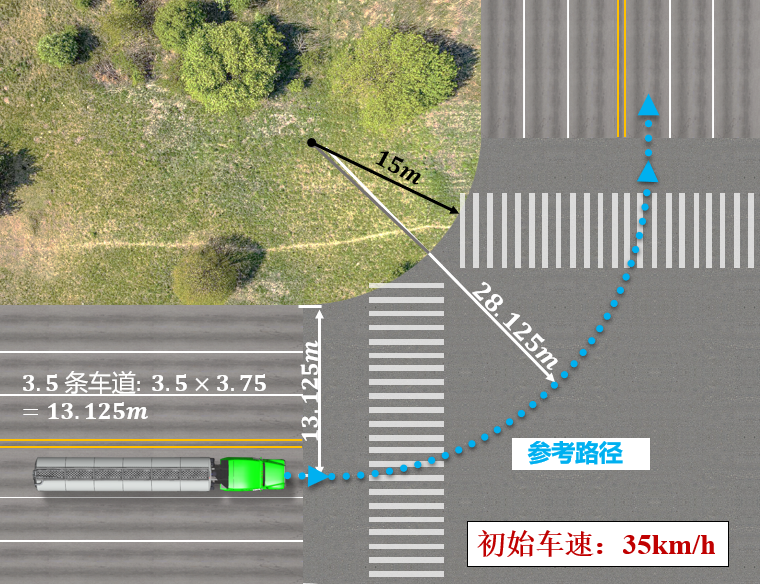
\includegraphics[width=0.54\linewidth]{fig/chap4/s_corner_illust.png}}
            \subcaptionbox{左转弯工况跟踪情况分析 \label{fig:s_corner_track}}
                {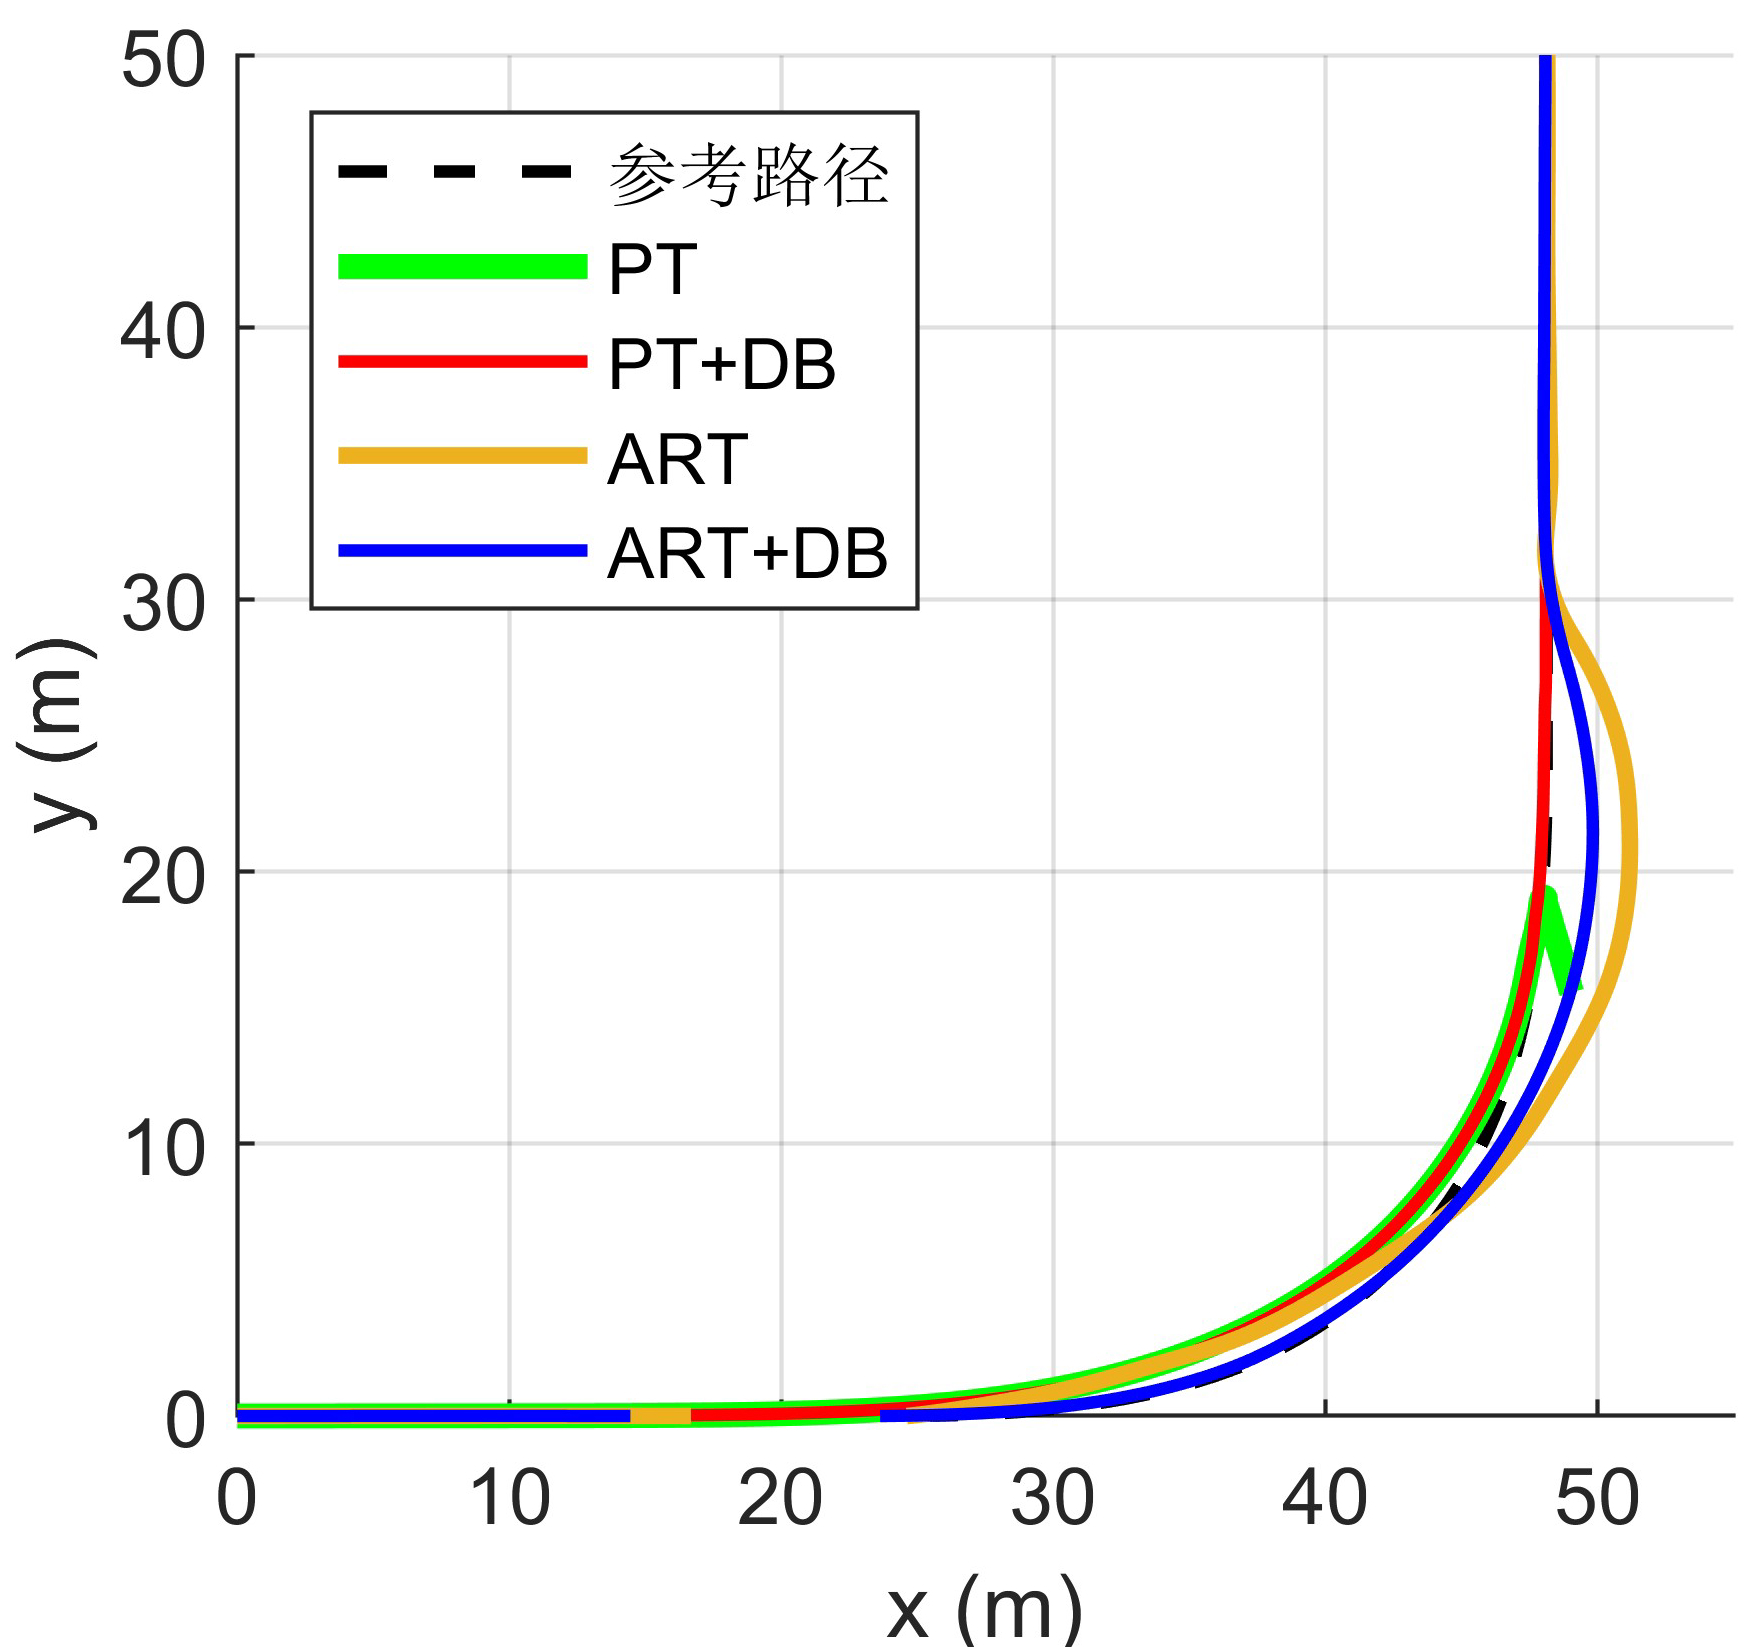
\includegraphics[width=0.45\linewidth]{fig/chap4/s_corner_traj.jpg}}
            \caption{左转弯工况场景设置与轨迹跟踪结果}
            \label{fig:s_corner_illust_and_track}
            \end{figure}
            \begin{figure}
            \centering
            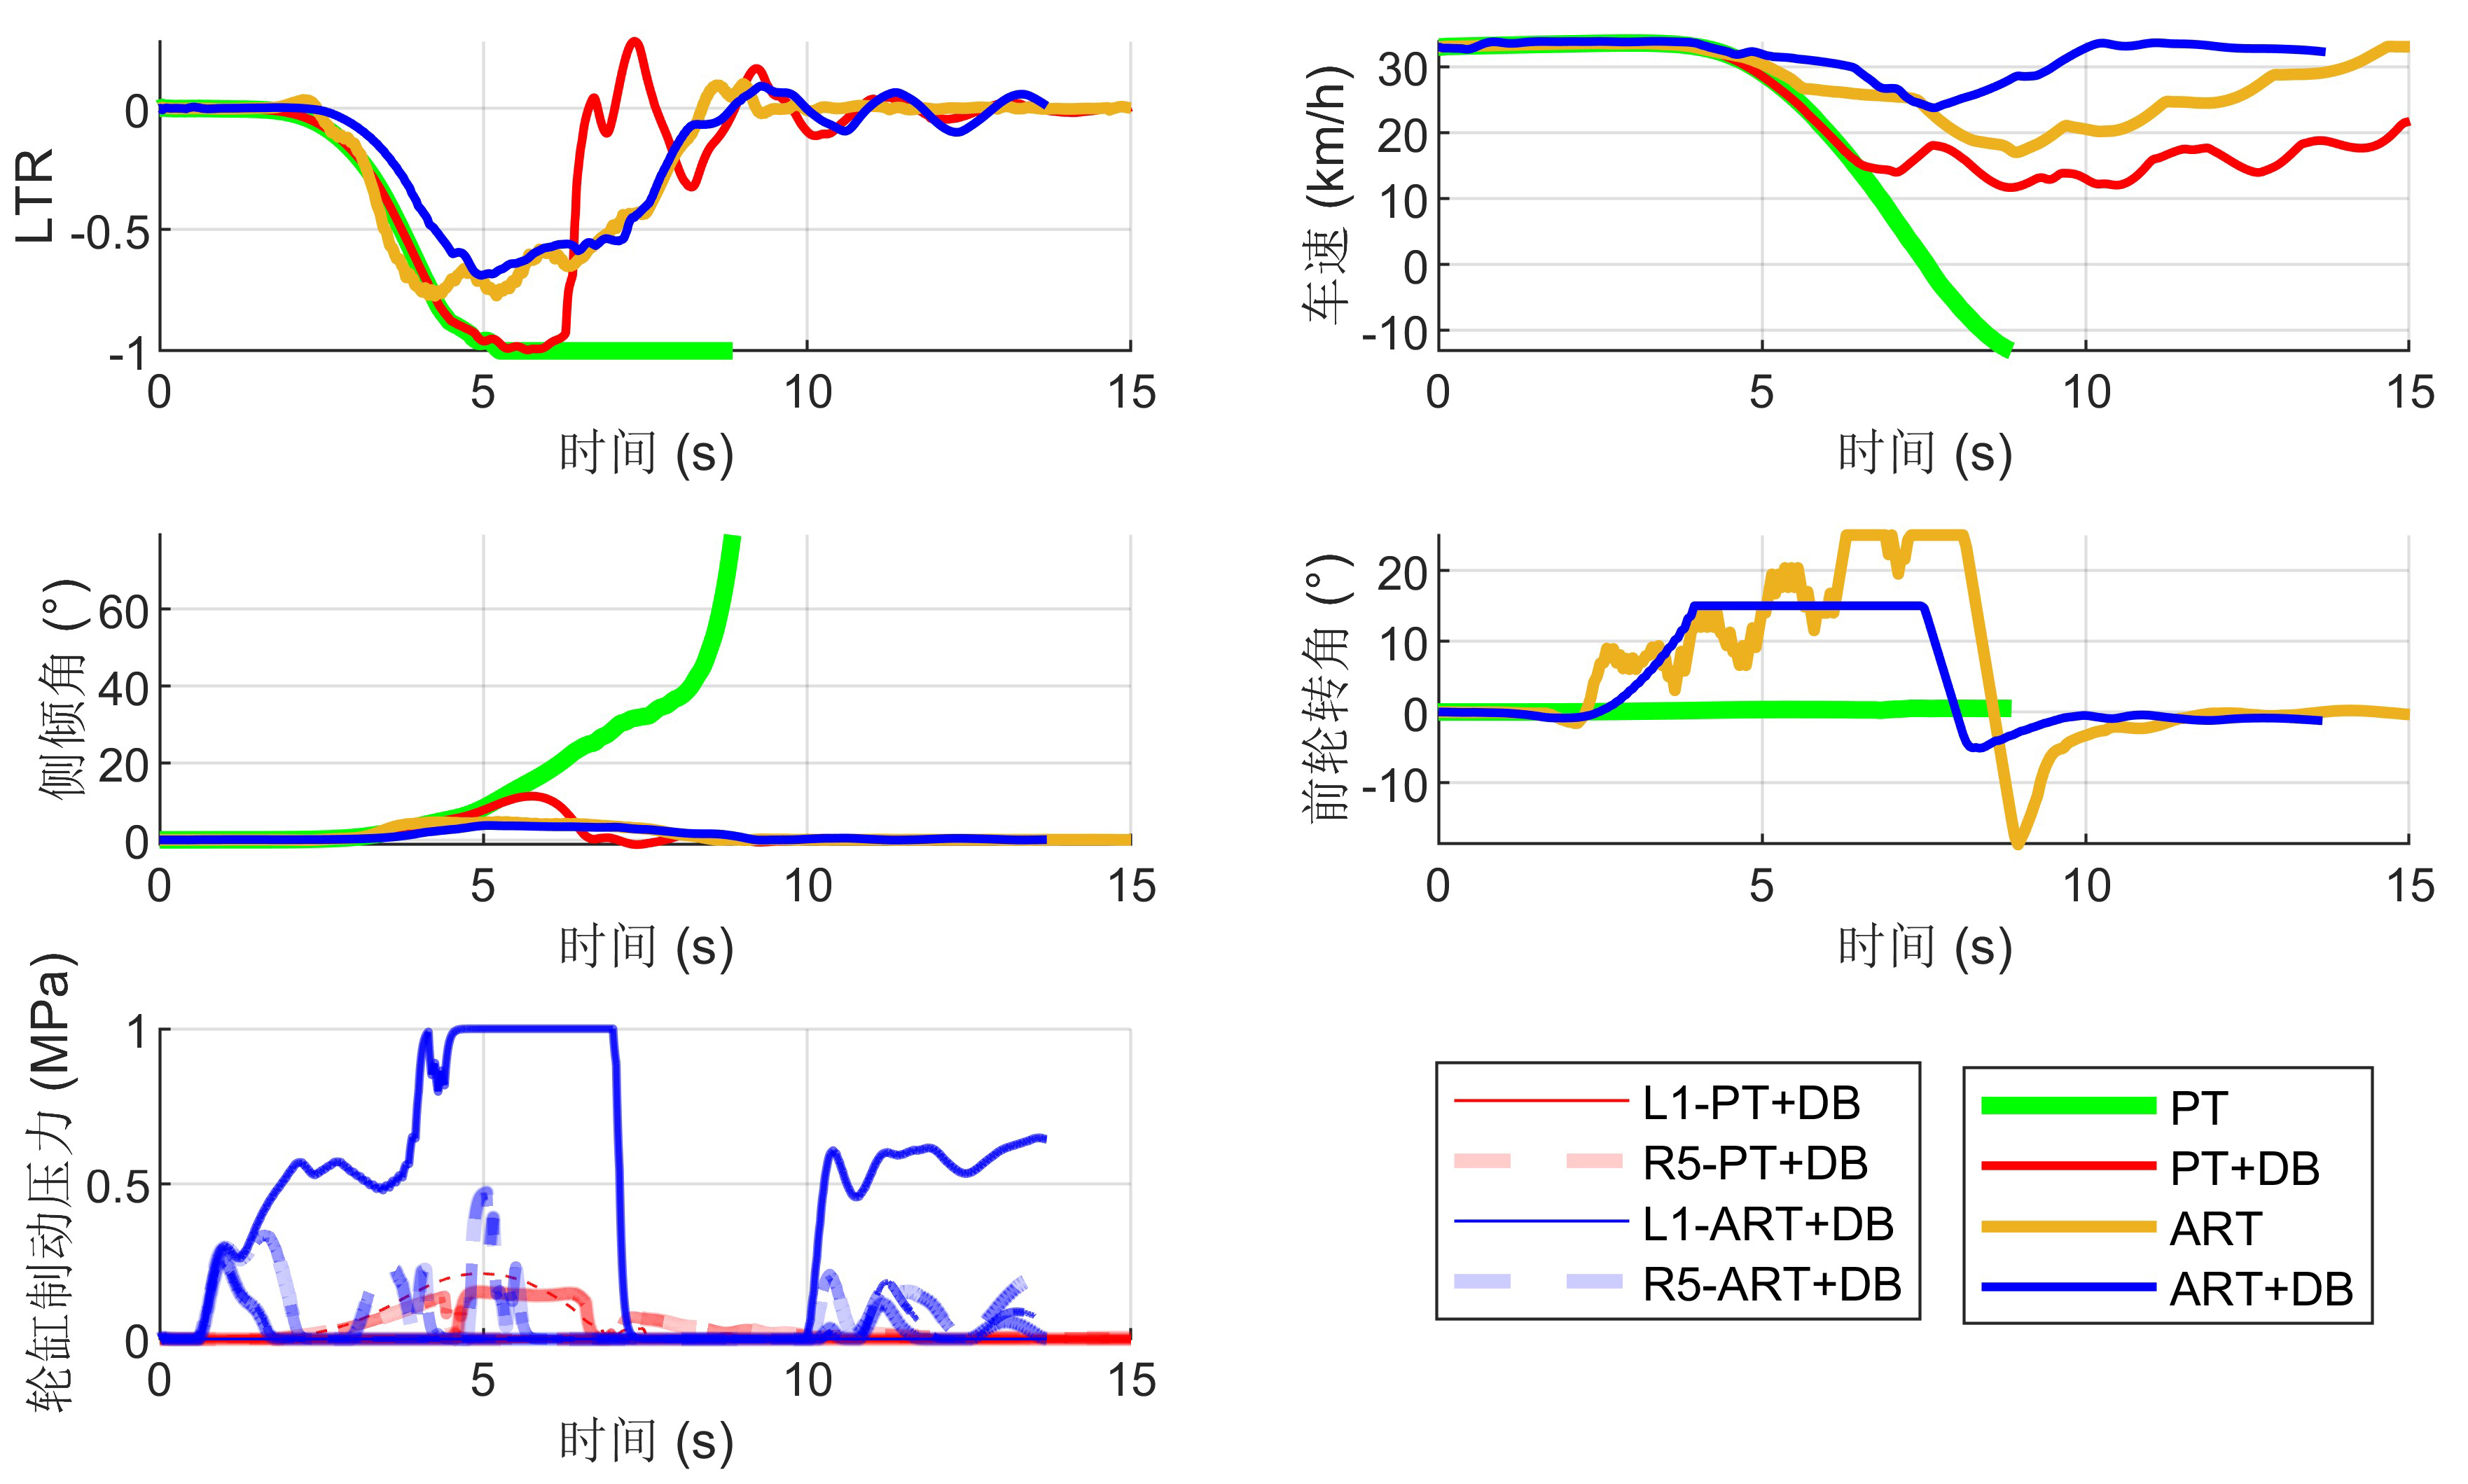
\includegraphics[width=1.0\linewidth]{fig/chap4/s_corner_xu.jpg}
            \caption{左转弯工况车辆状态与控制量变化趋势}
            \label{fig:s_corner_xu}
            \end{figure}
            

            
            在转向控制上，ART由于无法通过制动抵消晃动导致只能通过转角抵消晃动，这让转角变化过程不够稳定；在制动控制时，ART+DB倾向于较多使用制动，这也是本方法的一个缺点，即并不够节能。ART+DB组在使用了如此多制动的情况下速度损失却最少的原因在于，MPC模型内部已经考虑差动制动对纵向速度的影响，且可以通过期望速度调控来增加传动系统输出。此时单侧制动的同时另一侧未受影响的车轮将负责持续输出更大的扭矩，实现了类似分布式驱动的效果，即一侧车轮制动一侧车轮驱动，整体效果为几乎对速度不产生影响的额外横摆力矩。
            


        \subsubsection{高速单移线工况}
        \label{subsub:slc}
            高速单车道变道（Single Lane Change, SLC）场景依据SAE-J2179标准设置，如图~\ref{fig:s_slc_illust}所示。初始车速设定为\SI{88}{km/h}，要求在\SI{61}{m}范围内完成向左侧宽度为\SI{4.392}{m}车道的变道操作。采用三阶Hermite插值法对关键点进行插值处理，确保参考路径曲率平滑变化。
            \begin{figure}
            \centering
            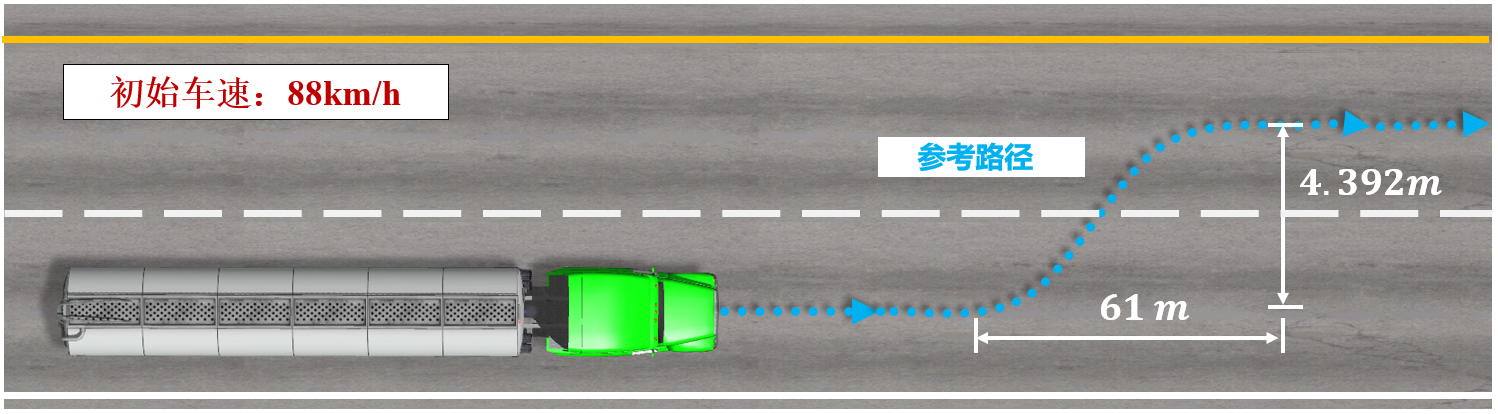
\includegraphics[width=0.8\linewidth]{fig/chap4/s_slc_illust.png}
            \caption{单移线工况场景设置}
            \label{fig:s_slc_illust}
            \end{figure}
            \begin{figure}
            \centering
            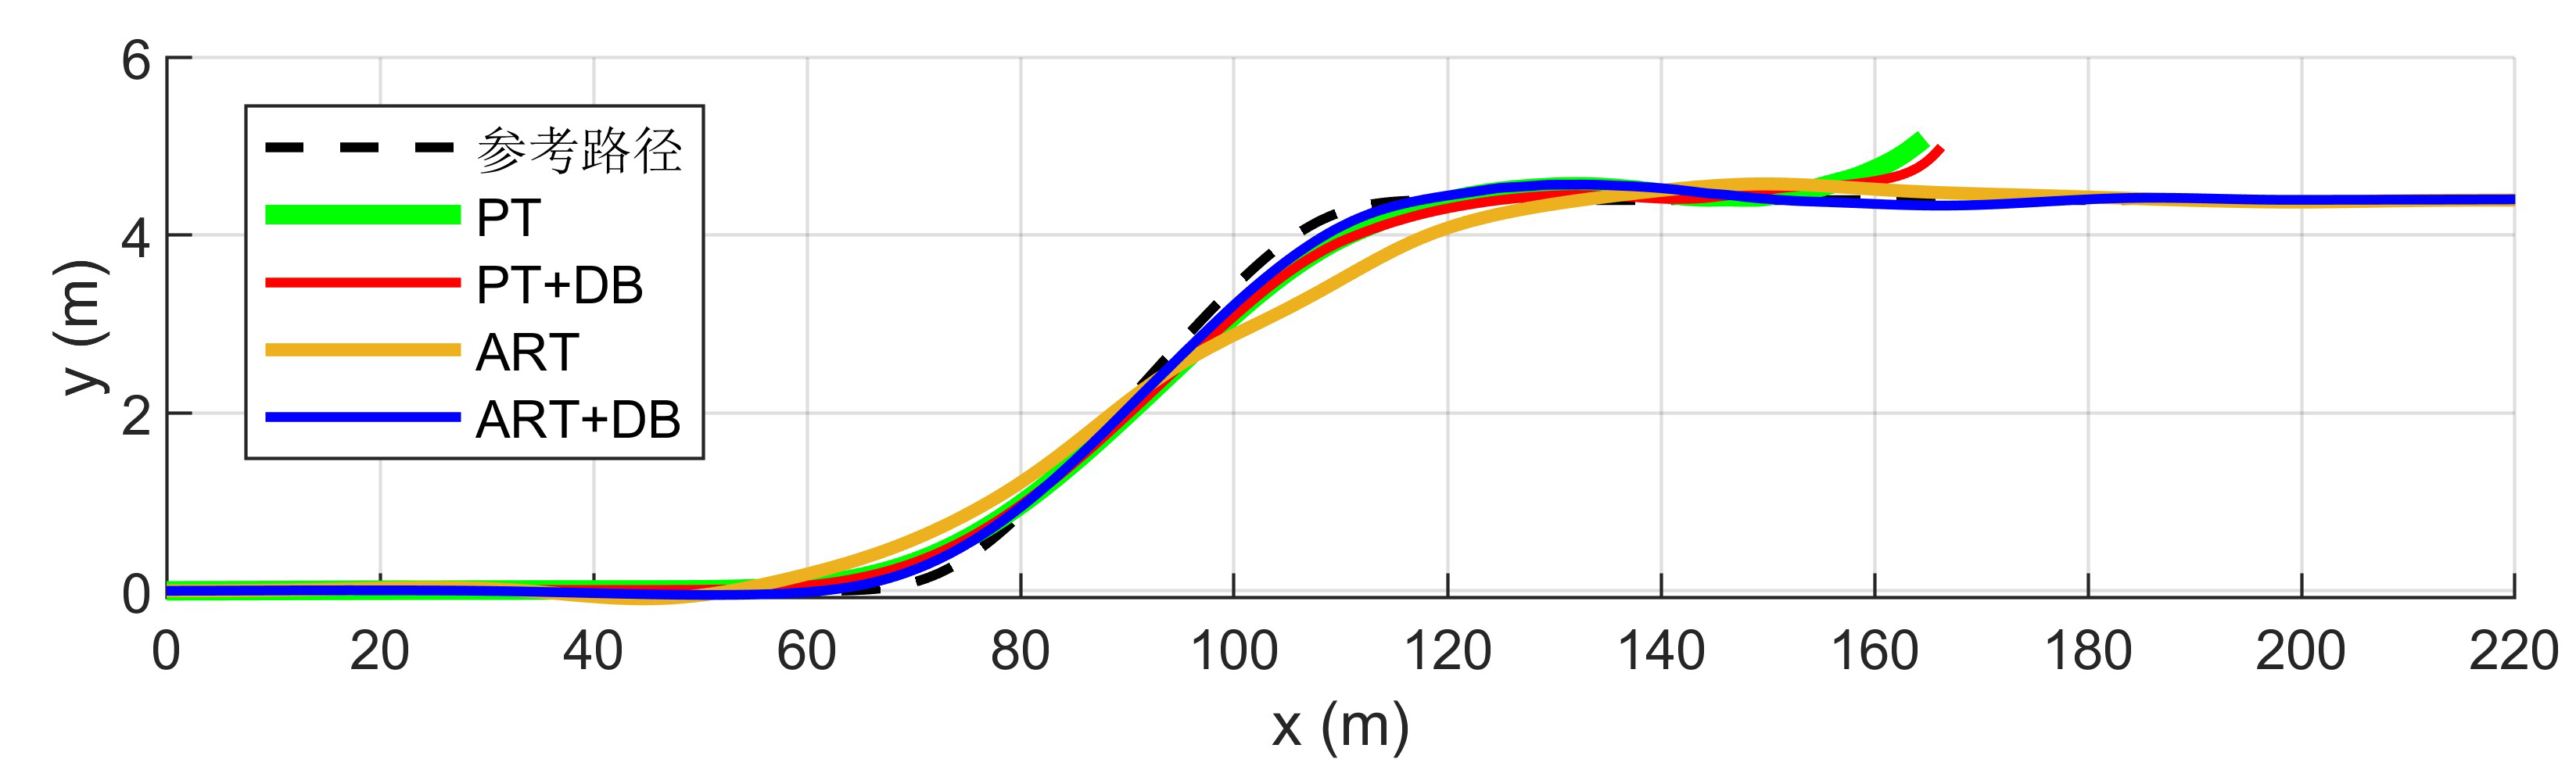
\includegraphics[width=0.8\linewidth]{fig/chap4/s_slc_traj.jpg}
            \caption{单移线工况跟踪情况分析}
            \label{fig:s_slc_track}
            \end{figure}
            图~\ref{fig:s_slc_track}结果表明，ART+DB组跟踪效果良好；为防止侧翻，ART组在\SI{50}{m} 处（变道动作发生前）即开始进行小幅转向调整但受极端工况及MPC控制器施加的软约束（$|\text{LTR}_{eql}| < 0.75$）影响，控制器以牺牲部分跟踪性能为代价保障防侧翻安全；PT和PT+DB组在发生侧翻前跟踪效果良好。
            
            车辆状态变化如图~\ref{fig:s_slc_xu}所示，PT与PT+DB在变道完成后的第\SI{6}{s}均发生侧翻。防侧翻控制组虽牺牲了部分跟踪性能，但跟踪误差仍处于可接受范围，且始终将LTR维持在安全区间内。在速度控制上，ART只进行转向控制，故基本未损失速度；而ART+DB由于控制考虑横纵向耦合，通过施加差动制动时增加对应期望速度，从而同样基本未损失速度；PT并没有制动控制，故在侧翻前同样未损失速度；PT+DB即便启用差速制动后，车速被降至\SI{50}{km/h}左右，仍无法避免侧翻事故的发生，这是由于差动制动直到接近侧翻状态才介入，已无法扭转即将侧翻的现状。
            \begin{figure}
            \centering
            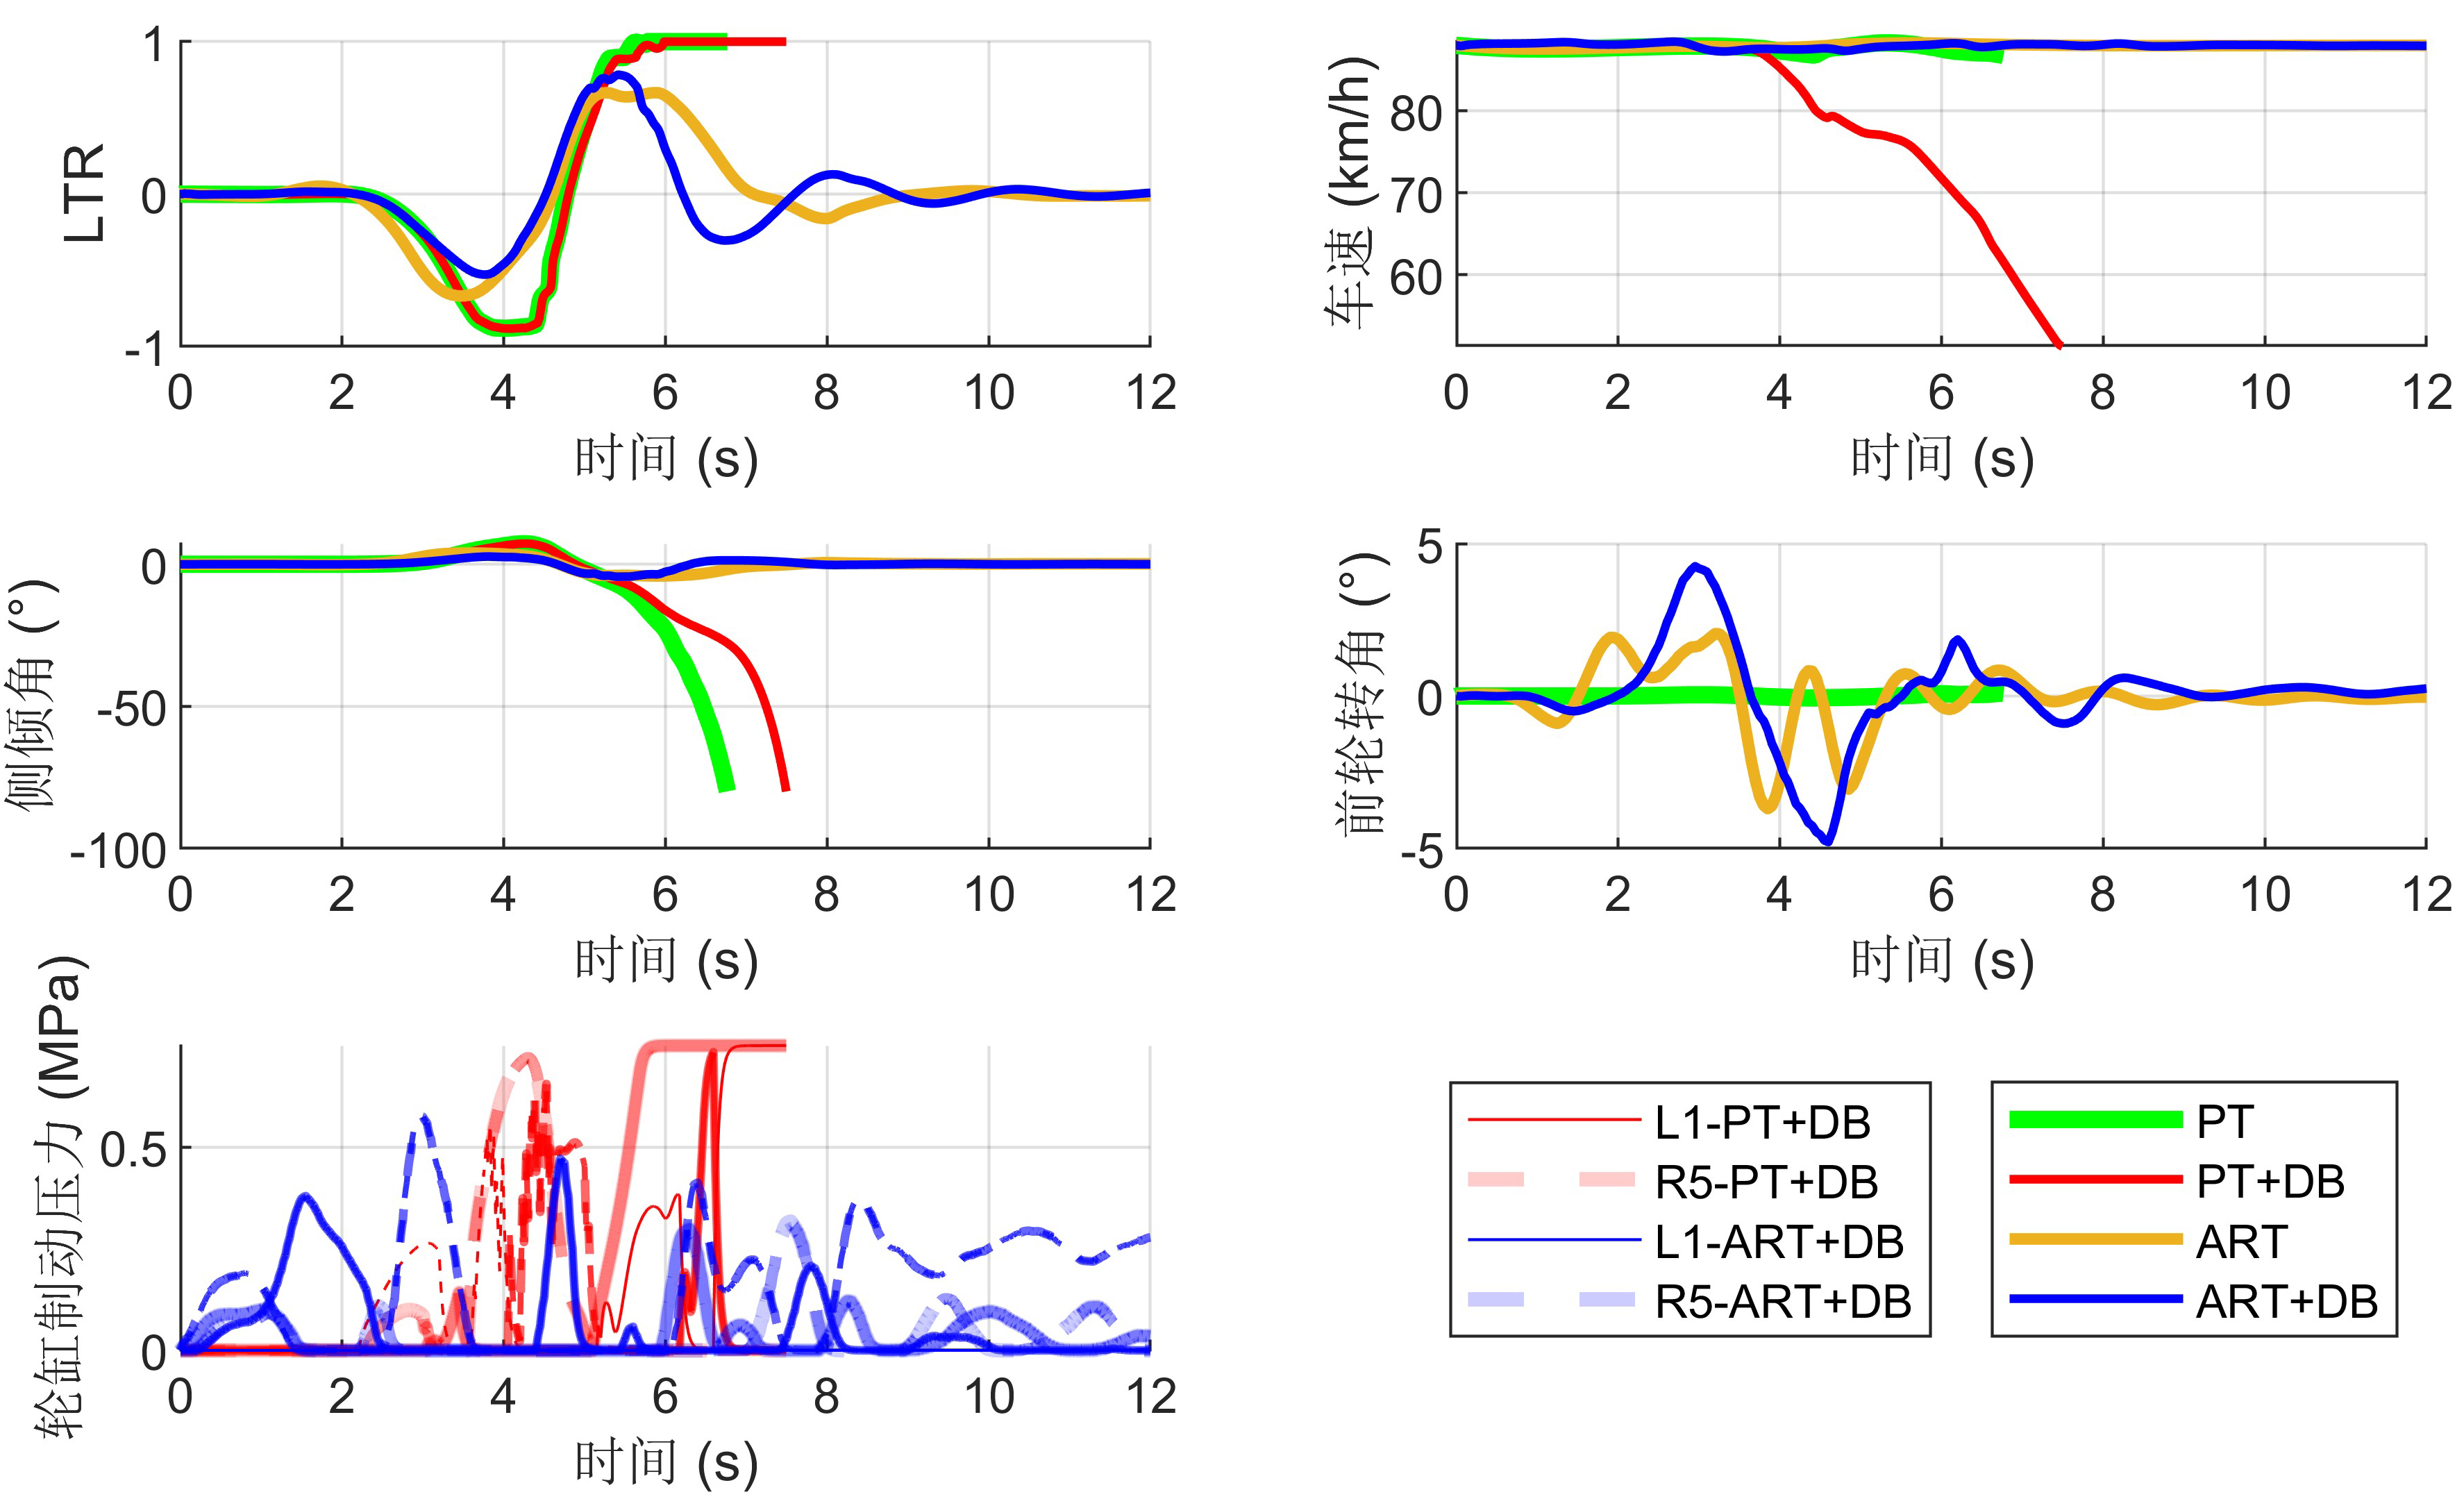
\includegraphics[width=1.0\linewidth]{fig/chap4/s_slc_xu.jpg}
            \caption{单移线工况车辆状态与控制量变化趋势}
            \label{fig:s_slc_xu}
            \end{figure}
            在控制量变化上，ART需通过转向控制来抵消晃动，故出现了转向指令频繁波动的情况；ART+DB在前段通过左右不断变化的差动制动来抵消晃动，转向角则保持平稳，加之MFASMC的跟踪误差补偿，使得跟踪更加精确；在轨迹跟踪结束后，ART+DB组通过持续差动的方式来抑制换道过程中产生的晃动，辅助车辆更快恢复稳定状态。对于PT+DB组，其制动在换道开始时才介入，已经为时已晚。


            根据本场景仿真可进一步发现，差动制动的引入可以在进入危险工况时提高车辆侧翻稳定性边界、保持车辆稳定，并在从危险工况恢复后抑制晃动、帮助车辆快速恢复平稳状态。



        \subsubsection{短距双移线工况}
        \label{subsub:dlc}
            短距双车道变换（Double Lane Change, DLC）工况如图~\ref{fig:s_dlc_illust}所示，该工况下要求车辆以\SI{70}{km/h}的速度，在\SI{30}{m}距离内完成\SI{3.5}{m}的侧向变道，随后直线行驶\SI{30}{m}，再在\SI{30}{m}内驶回原车道。
            

            根据仿真试验，PT组在\SI{62}{km/h}的速度下即发生侧翻，表明本研究设定的\SI{70}{km/h}试验速度具有较高风险。轨迹跟踪情况如图~\ref{fig:s_dlc_track}所示，PT组在\SI{70}{km/h}的初速度下，在约第\SI{6}{s}发生侧翻，其他所有组均未发生侧翻；PT+DB组维持相同轨迹，跟踪情况较好；ART组在\SI{60}{m}处提前开始转向，减小了变道幅度，并提前缓慢换回，整体牺牲了很多跟踪精度；ART+DB组轨迹基本与PT+DB组相同，跟踪效果较好。

            \begin{figure}
            \centering
            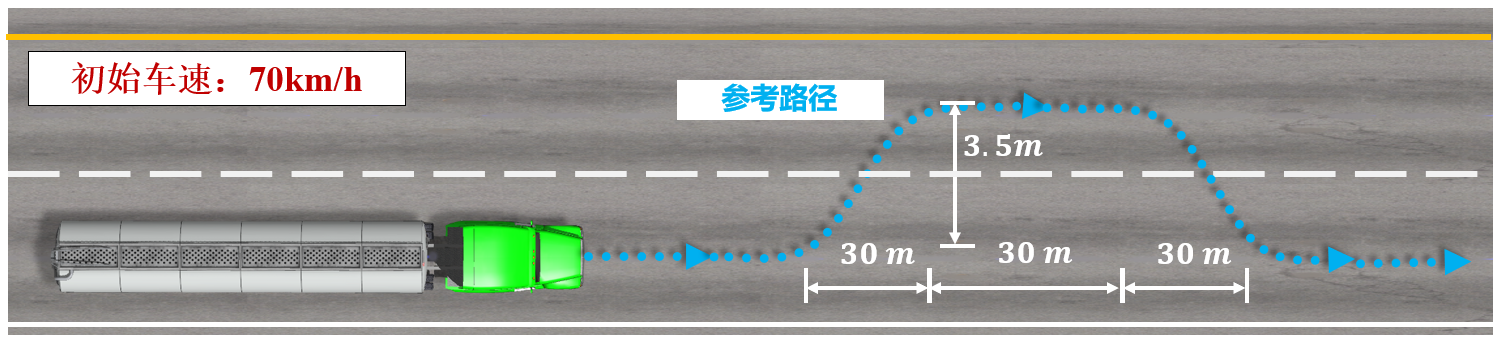
\includegraphics[width=0.85\linewidth]{fig/chap4/s_dlc_illust.png}
            \caption{双移线工况场景设置}
            \label{fig:s_dlc_illust}
            \end{figure}
            \begin{figure}
            \centering
            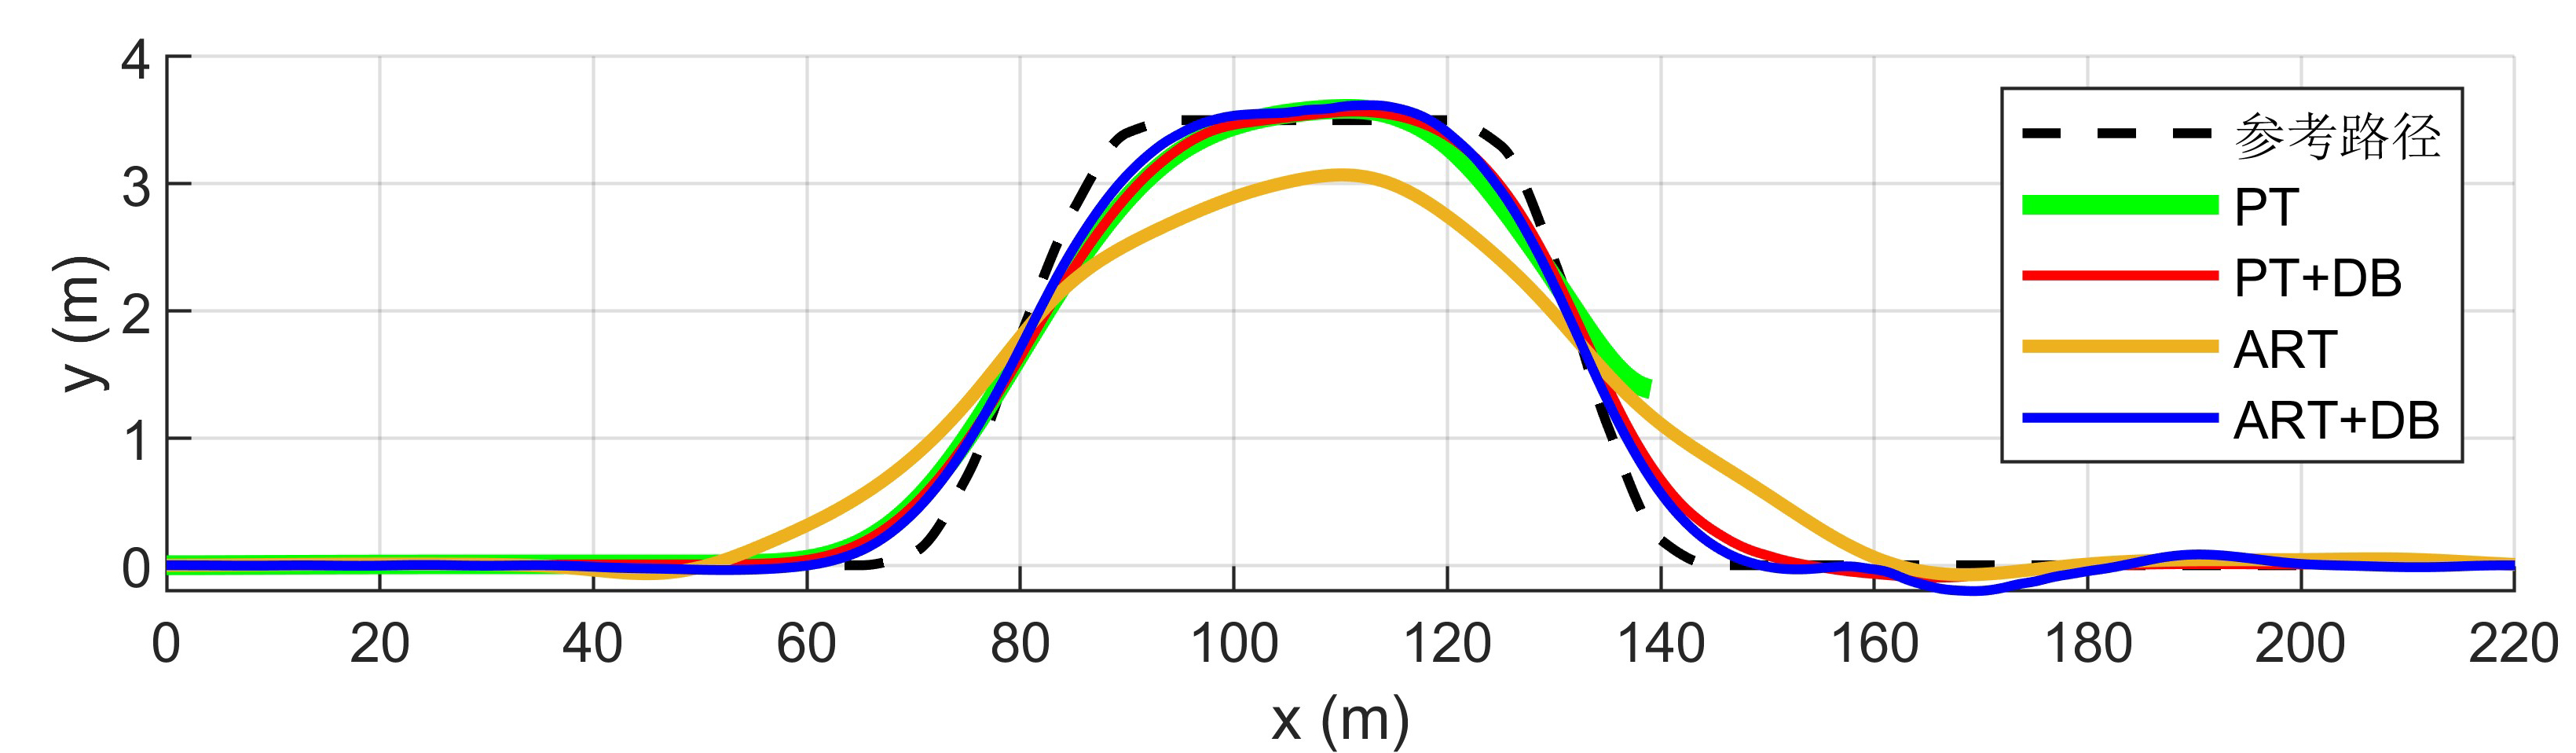
\includegraphics[width=0.8\linewidth]{fig/chap4/s_dlc_traj.jpg}
            \caption{双移线工况跟踪情况分析}
            \label{fig:s_dlc_track}
            \end{figure}
            \begin{figure}
            \centering
            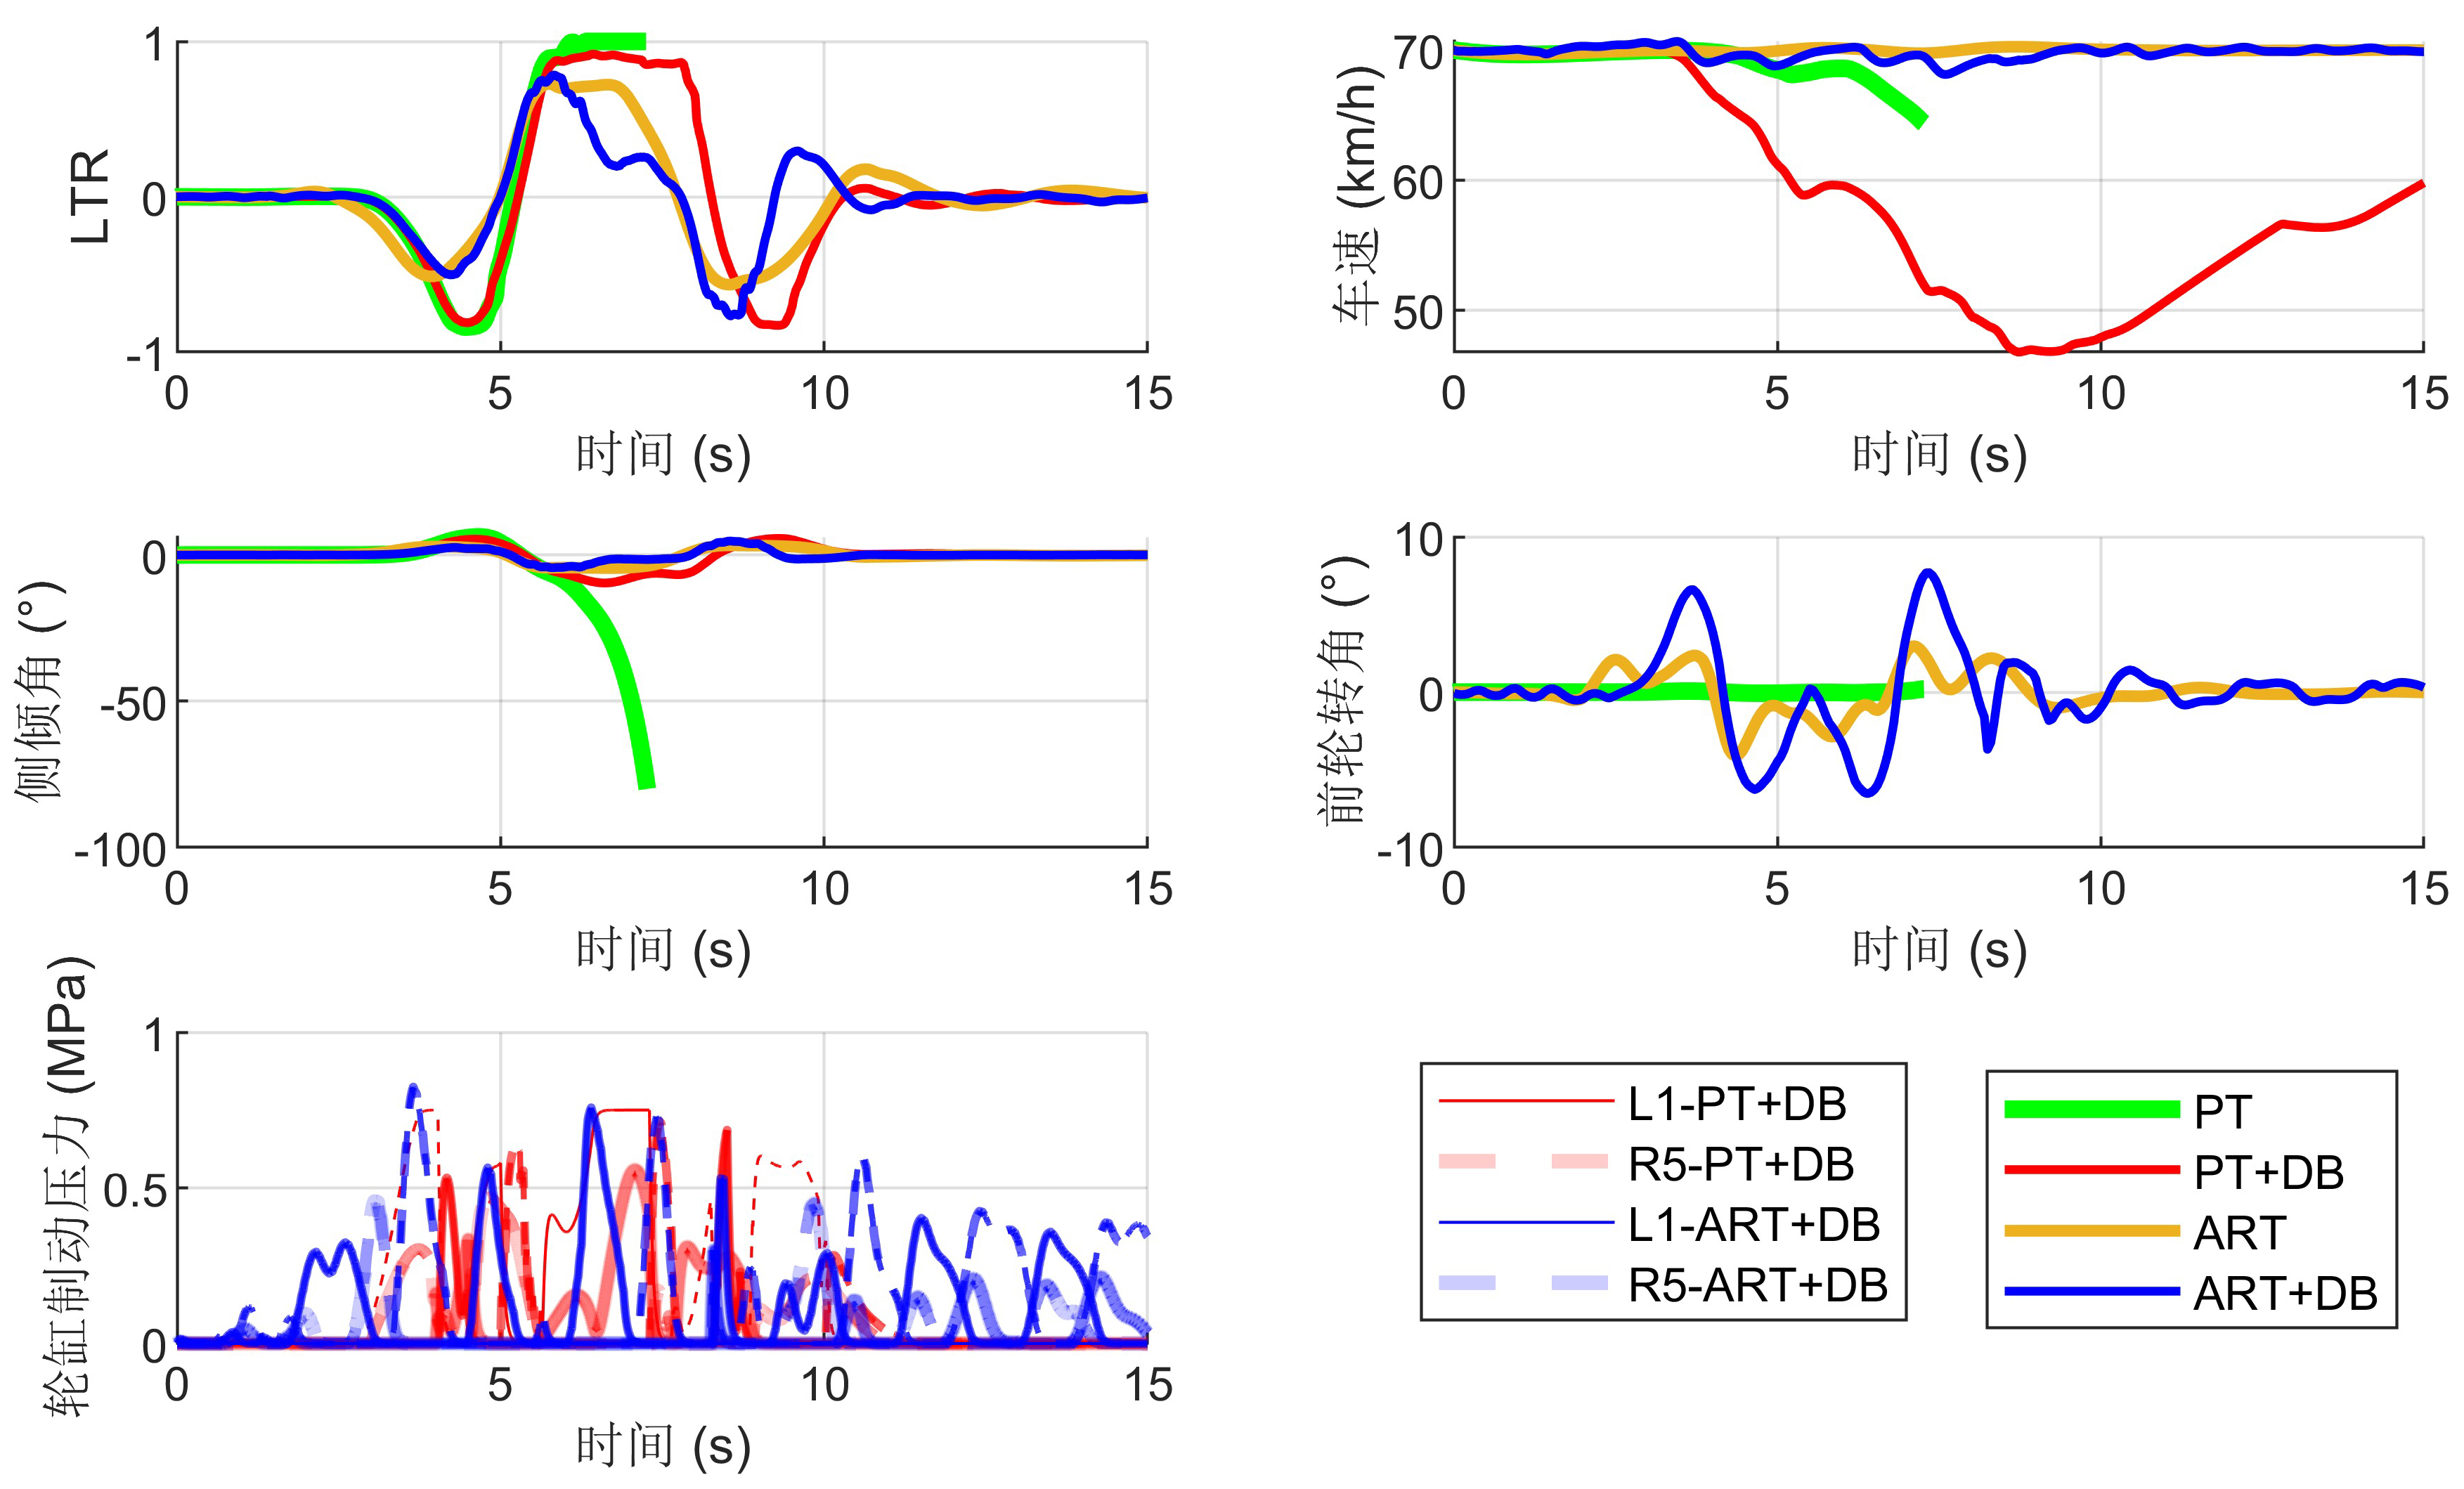
\includegraphics[width=1.0\linewidth]{fig/chap4/s_dlc_xu.jpg}
            \caption{双移线工况车辆状态与控制量变化趋势}
            \label{fig:s_dlc_xu}
            \end{figure}

           双移线工况下车辆的状态变化如图~\ref{fig:s_dlc_xu}所示。在防侧翻效果上，如从LTR的变化可看出，PT+DB组在约第\SI{6}{s}几乎接近侧翻，且这一状态维持了约\SI{2.5}{s}，仍然相当危险，单独采用差速制动的方案，虽能避免侧翻，但LTR会在至少\SI{2.5}{s}内达到饱和，且车速大幅降低引发纵向液体晃动，进而产生新的问题；ART组将\(\text{LTR}_{eql}\)控制在软约束范围内，从而在极限工况下避免了侧翻；ART+DB方法同样将\(\text{LTR}_{eql}\)控制在软约束范围内，虽然跟踪精度相较于ART高了很多，且并没有牺牲对LTR状态的控制。
           
           控制量变化上，ART组由于只能通过减小转角来在尽量满足不侧翻约束的前提下跟踪轨迹，故整体转向角度变化最小；PT+DB组在开始换道时采用差动制动介入，但其介入时机较晚，无法阻止LTR的快速增加；ART+DB组则在换道前，从第\SI{2}{s}开始就进行了差动控制，此时前轮转角仍然接近0，其作用在于根据期望轨迹提前让液体向能抵消换道时产生晃动的方向晃动，从而显著减小了LTR的第一个峰值，进而使得第二个峰值可控；同时ART+DB组利用差动制动与纵向期望速度控制结合，在几乎不降低车速的情况下维持了高精度的轨迹跟踪，在双移线结束后通过连续差动制动对罐内液体晃动进行主动抑制。

        
        \subsubsection{麋鹿工况救车实验}  
        \label{subsub:deer}
            半侧翻模态即一侧车轮离地时的车辆状态，通过现实中的实例可确定，半侧翻模态下存在状态子空间，可通过前轮转角完全控制\cite{KomasaQi2026MasterThesis_repo}；第\ref{chap:architecture}章\ref{subsubsec:resource_analysis}小节明确了车端需要具备规控降级能力，需确保在驾驶员误操作/绊倒性侧翻等特殊情况下车辆不可避免地已经陷入半侧翻状态时，车辆仍然具备一定的自救能力。

            本小节描述了麋鹿工况救车实验，实验场景如图~\ref{fig:s_deer_illust}所示。该场景模拟车辆以\SI{80}{km/h}行驶且车上存在安全员时，道路左侧突然出现横穿目标，安全员紧急向右猛打方向并随后回正的情况。车辆在第\SI{4.7}{s}左侧车轮完全离地，进入半侧翻状态。本文在此刻切换控制器，用以检验控制器能否在强非线性半侧翻工况下实现防侧翻救车。

            \begin{figure}
            \centering
            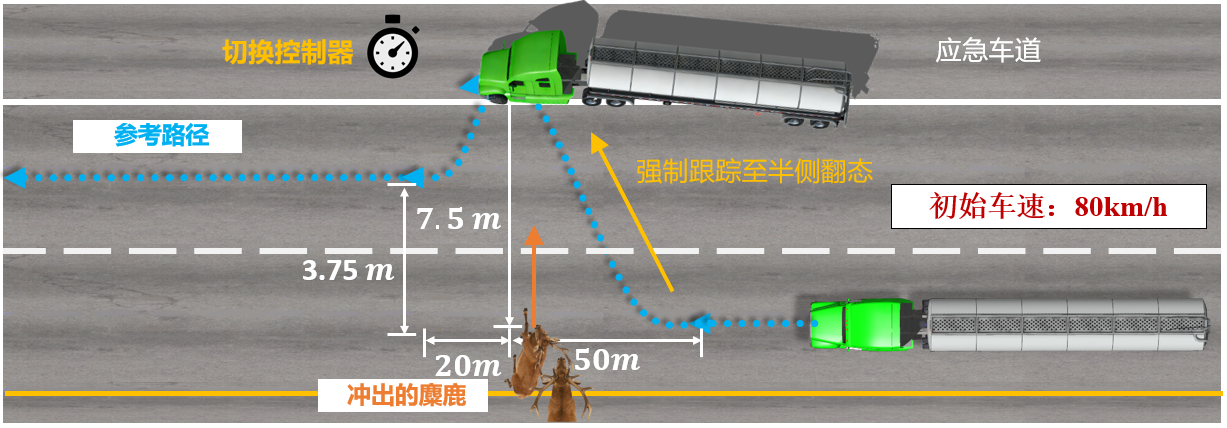
\includegraphics[width=0.8\linewidth]{fig/chap4/s_deer_illust.png}
            \caption{麋鹿工况场景设置}
            \label{fig:s_deer_illust}
            \end{figure}

            轨迹跟踪情况如图~\ref{fig:s_deer_track}所示，PT组和PT+DB组由于没有考虑防侧翻的转向控制，在打回方向时仍然向着目标轨迹靠近，故直接发生了侧翻；ART组在切换控制器后果断选择了反打方向朝着远离目标轨迹的方向，但由于没有车速控制，此时车辆的状态已经超过了单纯依靠前轮转角可控的边界，故继续向前行驶并仍然发生了侧翻；ART+DB组在ART组基础上加入了差动制动，此时车辆不仅迅速反打方向逆操舵，而且猛烈制动。此时并没有对向车轮，全部轮胎纵向力用来给车辆减速并提供横摆力矩，车辆减慢速度的同时继续远离期望轨迹，并在摆脱半侧翻状态后迅速靠近期望轨迹，恢复了正常跟踪。

            \begin{figure}
            \centering
            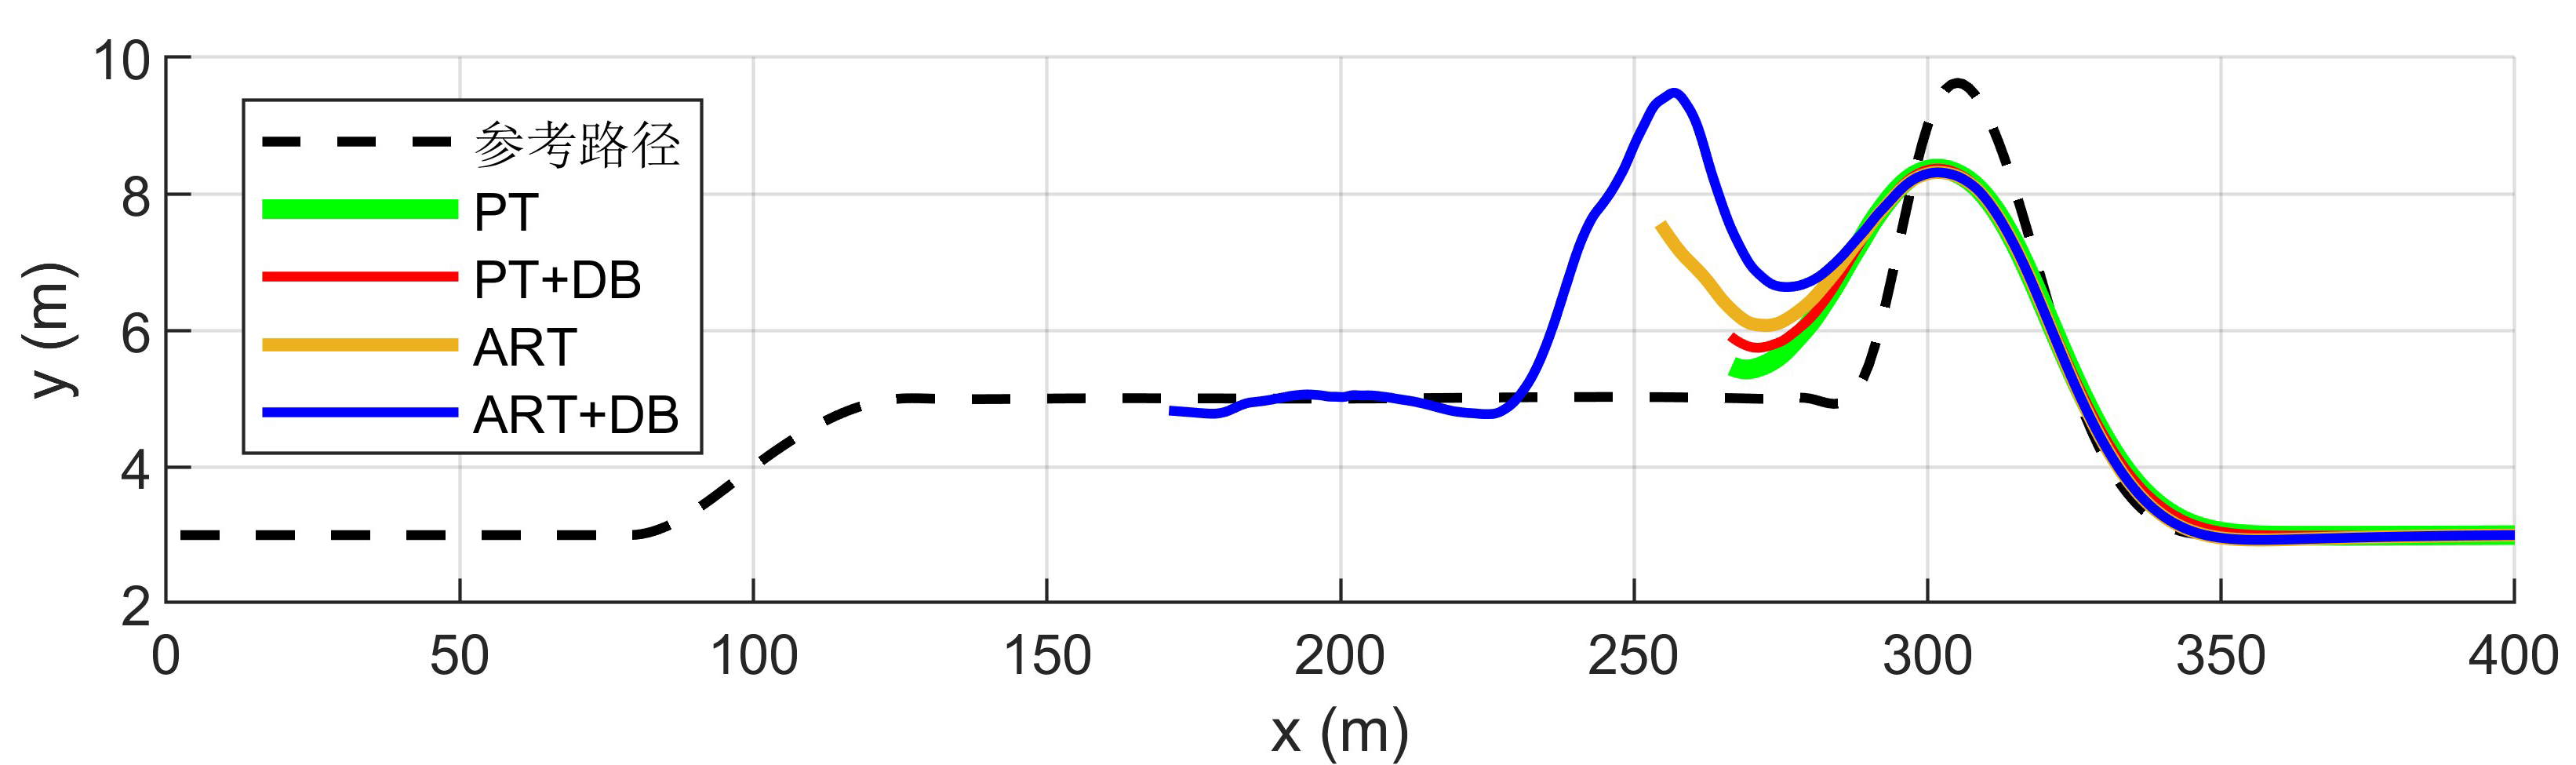
\includegraphics[width=0.85\linewidth]{fig/chap4/s_deer_traj.jpg}
            \caption{麋鹿工况跟踪情况分析}
            \label{fig:s_deer_track}
            \end{figure}
            \begin{figure}
            \centering
            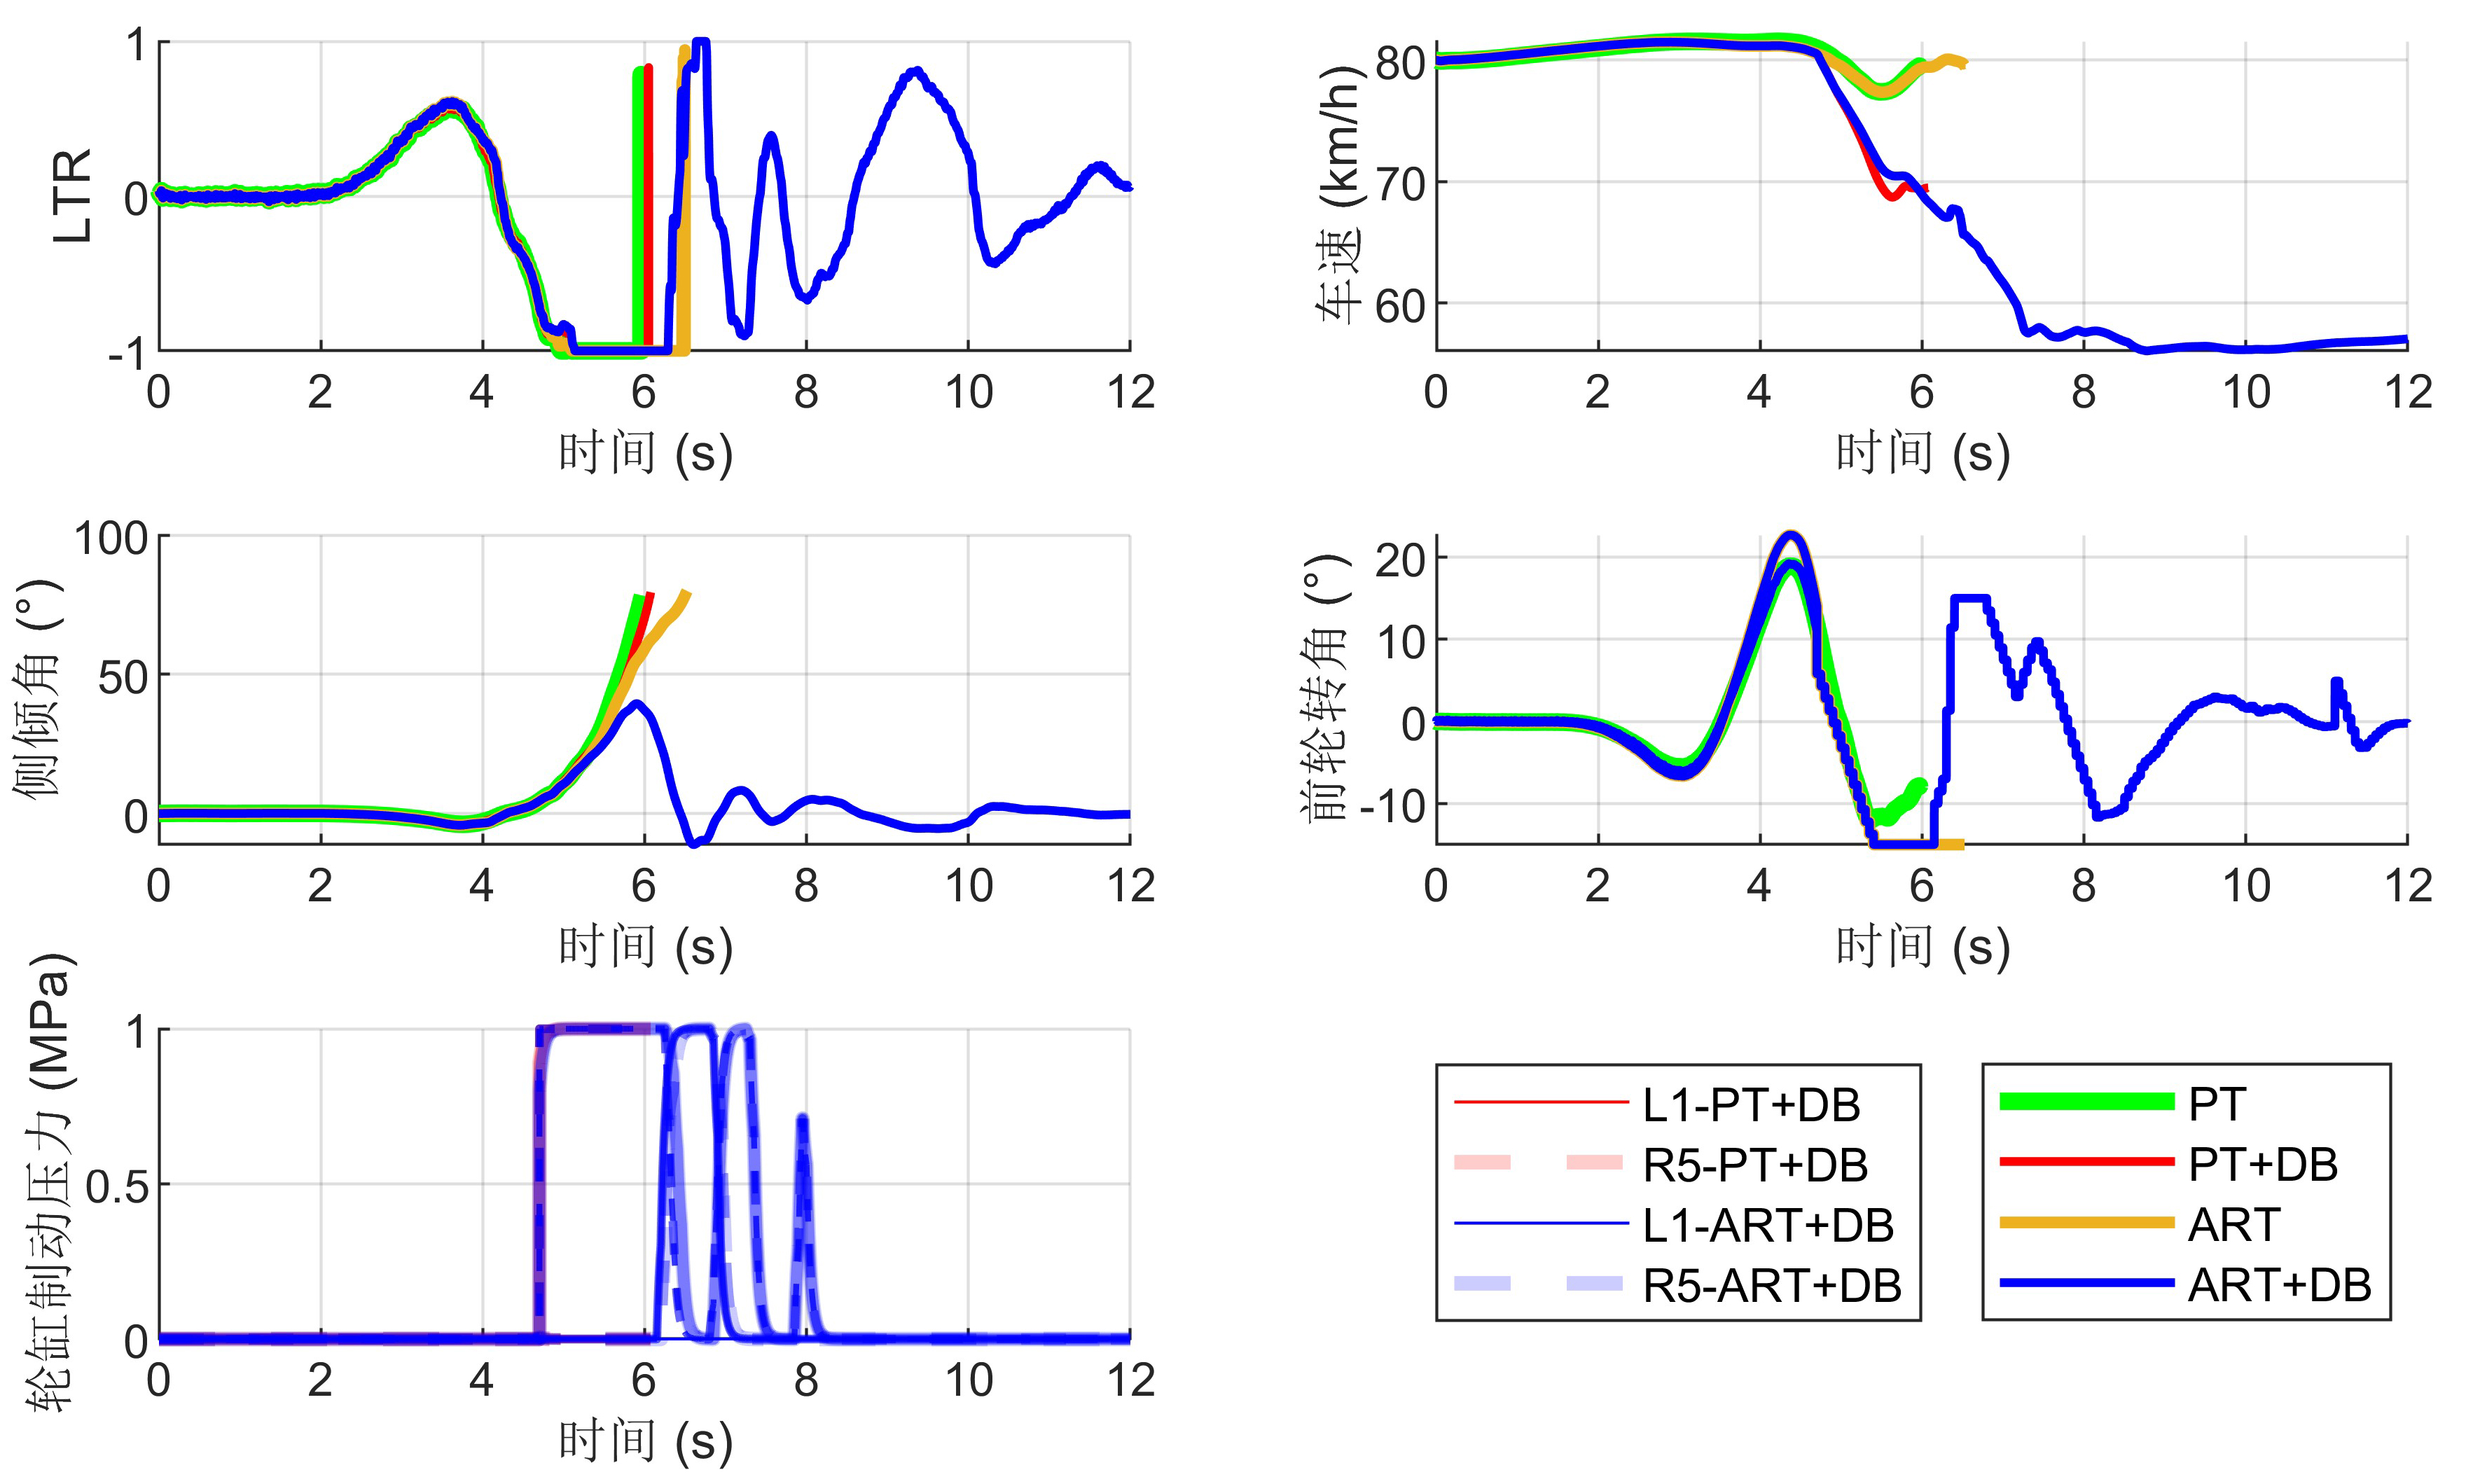
\includegraphics[width=1.0\linewidth]{fig/chap4/s_deer_xu.jpg}
            \caption{麋鹿工况车辆状态与控制量变化趋势}
            \label{fig:s_deer_xu}
            \end{figure}

            车辆状态及控制量变化如图~\ref{fig:s_deer_xu}所示，ART组由于反打方向，侧翻时间相较于PT和PT+DB组更加延后，但没有减速所以ART组的车速基本维持在了初始速度\SI{80}{km/h}左右，这是其最终未能摆脱侧翻结果的决定性因素。控制输入上，PT+DB组与ART+DB组进行了相同的全力减速，但由于并没有进行逆操舵，故虽然速度降低了，但仍然走向了侧翻的结果。


    \subsubsection{仿真结果分析}        
    \label{subsub:simu_analysis}
        综合左转弯、高速单移线、短距双移线3个典型极限工况及麋鹿救车特殊极限工况的仿真验证结果，可系统归纳出以下结论：
        \begin{enumerate}
            \item \emph{液罐车侧翻风险的特殊性}：普通车辆能够顺利跟踪的行驶路径，对于部分装载状态下的液罐车仍可能引发侧翻，其核心诱因是罐内液体晃动与车辆动力学的耦合效应，因此液罐车轨迹跟踪控制需将防侧翻作为核心约束，而非仅关注路径跟踪精度。
            \item \emph{侧翻评价指标的有效性}：由悬架力计算得到的等效载荷转移率 $\text{LTR}_{eql}$ 与TruckSim轮胎力实际计算的载荷转移率 LTR 吻合度较高，能够准确反映车辆的侧翻动力学特性，可作为自动驾驶场景下液罐车防侧翻控制的核心评价与约束指标。
            \item \emph{软约束+MPC的基础控制效果}：通过对 $\text{LTR}_{eql}$ 施加 $|\text{LTR}_{eql}| < 0.75$ 的软约束，控制器可在保证罐内液体近似线性晃动、轨迹跟踪性能满足工程可接受范围的前提下，主动规划转向动作以避免液罐车侧翻，验证了多约束MPC框架在防侧翻轨迹跟踪中的可行性。
            \item \emph{单一控制手段的局限性}：
                \begin{itemize}
                    \item 单纯差动制动（如PT+DB）对车辆抗侧翻能力的提升有限，且仅在侧翻风险临近时介入无法扭转侧翻趋势，同时单独使用会造成车速大幅下降，还可能引发纵向液体晃动等新问题；
                    \item 单纯转向控制（如ART）需通过牺牲更多轨迹跟踪精度、增大转向指令波动来抵消液体晃动，无法充分拓展车辆侧翻稳定边界。
                \end{itemize}
            \item \emph{横纵向耦合加补偿方案的协同优势}：
                \begin{itemize}
                    \item 在MPC中纳入纵向动力学后，可通过同步调整期望速度抵消差动制动对车速的影响，实现“单侧制动+单侧驱动”的分布式驱动等效效果，在几乎不损失车速的前提下提供额外横摆力矩；
                    \item 转向控制与差动制动的耦合（ART+DB）可提前介入抑制液体晃动，降低LTR峰值，同时通过MFASMC跟踪误差补偿减少轨迹偏移，兼顾了防侧翻安全性与轨迹跟踪精度；
                    \item 差动制动可在车辆从危险工况恢复后主动抑制罐内液体晃动，辅助车辆更快恢复稳定状态。
                \end{itemize}
            \item \emph{极端工况下的鲁棒性}：ART+DB控制器显著拓展了车辆的可控边界，即使在半侧翻模态（一侧车轮离地）这种超出常规LTR稳定性约束的极端工况下，仍可通过逆操舵与差动制动的协同控制实现救车，验证了该控制器在非线性极强的极限场景下的鲁棒性。
        \end{enumerate}

    \subsection{缩比模型车平台搭建}
        \label{sub:model_truck_platform}
        为进一步验证所提控制方案的可行性，本研究搭建了模型半挂液罐车实验平台并对车辆软件架构进行了设计与程序编写。本小节介绍半挂液罐车实验平台及实现防侧翻路径跟踪的程序架构。

        \subsubsection{车辆硬件配置}
            
            如图~\ref{fig:hardware}所示，模型主体为高精度1:14比例的TAMIYA半挂模型，尺寸为\SI{450}{mm}（长）×\SI{190}{mm}（宽）×\SI{350}{mm}（高）。安装液体罐后，整体尺寸保持为\SI{1250}{mm}（长）×\SI{200}{mm}（宽）×\SI{350}{mm}（高），模型总质量为\SI{42}{kg}，最大行驶速度约为\SI{3}{m/s}。平台配备防侧翻支架，可承受车辆最大\SI{15}{\degree}的倾斜，以防止实验过程中侧翻。

            \label{subsub:hardware}
            \begin{figure}
            \centering
            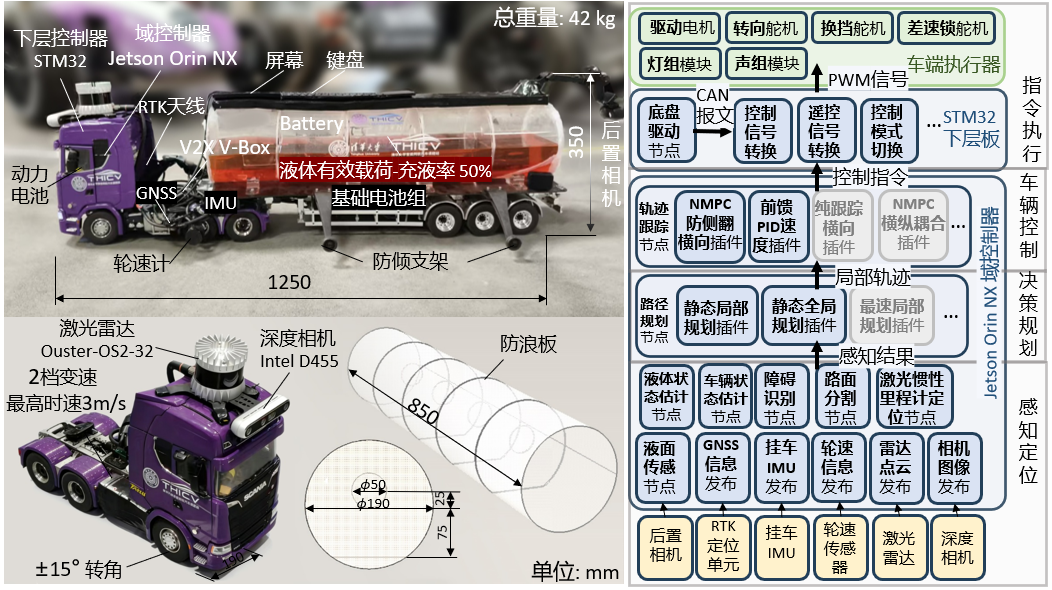
\includegraphics[width=1.0\linewidth]{fig/chap4/hardware.png}
            \caption{缩比模型车硬件配置}
            \label{fig:hardware}
            \end{figure}

            传感器配置包括：Ouster-OS2-32线激光雷达、英特尔D455深度相机用于环境感知；FDLink九轴惯性测量单元实现牵引车和挂车的位姿估计；WHEELTEC旋转编码器作为轮速传感器；后置摄像头用于记录液体运动。域控制器采用Jetson Orin NX（16GB RAM，100TOPS），各状态变量的测量方式如表~\ref{tab:state_measurement}所示。



            液体罐由厚度为\SI{5}{mm}的亚克力材料制成，内部间隔配置防晃板，模拟真实场景中常见的带防晃板液罐\cite{wanying2020antirolover}。该模型提供了集成化实验平台，可在接近真实世界的条件下验证液体罐车防侧翻控制算法。

            \begin{table}[htbp]
            \centering
            \caption{状态变量测量方法}
            \label{tab:state_measurement}
            \begin{tabular}{ll}
                \toprule
                状态变量 & 测量方法 \\
                \midrule
                \(v_{1y}, v_{2y}\) & 基于卡尔曼滤波估计\cite{FengRan2018} \\
                \(\psi, \theta_1\) & FDLink九轴GNSS（IMU+RTK） \\
                \(\dot{\psi}, \dot{\phi}_2, \dot{\phi}_2\) & FDLink九轴IMU \\
                \(\theta_1\) \(\theta_2\) & 状态估计器估算 \\
                \(Y_1, X_1, v_1\) & FDLink九轴GNSS（IMU+RTK） \\
                \(v_{1x}\) & WHEELTEC旋转编码器（作为轮速传感器） \\
                \bottomrule
            \end{tabular}
            \end{table}


        \subsubsection{自动驾驶软件设计}
            \label{subsub:software}
            车辆通过如图~\ref{fig:hardware}所示的程序架构实现防侧翻路径跟踪功能。感知层提供液体状态估计与目标级预测信息；决策与规划层基于预定义全局参考路径与路径重规划器进行决策；控制层主要由实现防侧翻路径跟踪的MPC组成。算法在机器人操作系统（Robot Operating System, ROS）Ubuntu 20.04环境下运行，其中MPC算法采用C++实现以保证实时性，其余节点大部分采用Python实现。本章全套控制算法与配套编写的定位、规划等自动驾驶代码开源于GitHub仓库HitchOpen-THICV-Stack中\cite{KomasaQi2025HitchOpen-THICV-Stack_repo}，配套算法经过2025年首届HitchOpen世界AI竞速锦标赛线上与天门山实车赛完善验证。


\section{模型试验与验证}
    \label{sub:model_experiment}
    本节基于上一节搭建的缩比例液罐车平台，推导了车辆动力学与流体动力学相似性原理，并开展了模型跟踪实验及前述最危险的双移线工况实验验证。

    \subsection{缩比模型相似性准则与工况设计}
        \label{subsub:similarity}
        相似性是采用模型替代原型开展试验的必要条件。对于同一物理过程，若两种现象在各对应点、对应时刻的物理量成比例，且矢量对应方向一致，则称这两种现象相似\cite{BookFluidMechanics}。采用模型车辆替代实车开展极限工况下的控制效果验证，需同时保证车辆动力学与流体动力学相似。

        本文中，车辆动力学相似特指侧翻动力学相似，可通过静态稳定系数（Static Stability Factor, SSF）定量表征。如图~\ref{fig:mod_similarity}所示，若模型的所有几何参数与质量分布均按比例系数$\lambda > 0$缩放，且实车与模型的静态稳定系数相同，则实车与模型仅在横向加速度相同时发生侧翻，即$ a_{y,vhl} = a_{y,mdl}$。但受实际条件限制，真实模型难以满足严格比例缩放条件，因此需引入修正系数$\lambda^{'}$

        \begin{equation}
        \lambda^{'} = \frac{SSF_{vhl}}{SSF_{mdl}} = \frac{T_{w,vhl}}{h_{cg,vhl}} \cdot \frac{h_{cg,mdl}}{T_{w,mdl}}
        \end{equation}

        即满足式\eqref{eq:similarity}时试验具有相似性
    
        \begin{equation}
        a_{y,vhl} = \lambda^{'}a_{y,mdl}
        \label{eq:similarity}
        \end{equation}

        \begin{figure}
        \centering
        \subcaptionbox{模型相似性条件\label{fig:mod_similarity}}
            {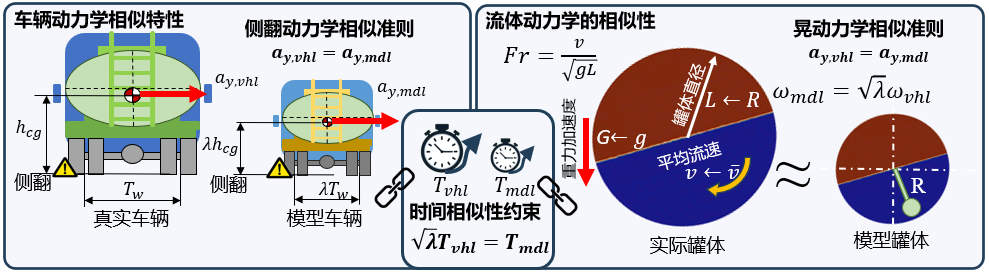
\includegraphics[width=1.0\linewidth]{fig/chap4/mod_similarity2.png}}
        \subcaptionbox{换道特征数与双移线设计\label{fig:lane_change_char}}
            {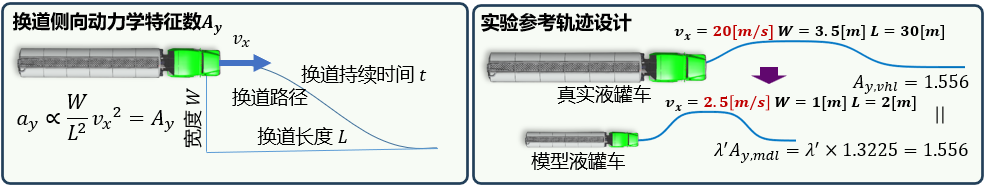
\includegraphics[width=1.0\linewidth]{fig/chap4/lane_change_char.png}}
        \subcaptionbox{模型车试验参考轨迹 \label{fig:exp_ref_traj}}
            {\includegraphics[width=1.0\linewidth]{fig/chap4/exp_ref_traj.jpg}}
        \caption{相似性准则与模型车试验参考轨迹设计}
        \label{fig:exp_ref_pic}
        \end{figure}


        对于带自由液面的流体，其流动主要受惯性力主导，因此采用弗劳德数$Fr$作为相似准则，其中$Fr = \frac{v_f}{\sqrt{gL}}$。式中$v_f$为流体特征速度，通常取平均流速$\bar{v_f}$；$g$为重力加速度，在横向激励下附加加速度较小，可认为$G=g$。罐体内部小幅线性晃动时，液体可近似为单摆，其摆长近似取罐体半径$R$。晃动频率$\omega$随$R$增大而降低，满足关系

        
        \begin{equation}
        \left. \omega \propto \sqrt{\frac{g}{R}}\Rightarrow\omega_{mdl} = \sqrt{\lambda}\omega_{vhl} \right.
        \end{equation}

        由上述关系可知，对于罐体液体晃动，只要横向加速度差异不大，合加速度即可近似为$g$。因此，实车罐体与模型罐体中液体的弗劳德数可认为相等，即

    
        \begin{equation}
        \begin{split}
        Fr_{mdl} &= \frac{v_{mdl}}{\sqrt{G_{mdl}L_{mdl}}} = \frac{\omega_{mdl}R_{mdl}}{\sqrt{gR_{mdl}}} 
        = \omega_{mdl}\sqrt{\frac{R_{mdl}}{g}}\\ &= \sqrt{\lambda}\omega_{vhl}\sqrt{\frac{R_{vhl}}{\lambda}} = \omega_{vhl}\sqrt{\frac{R_{vhl}}{g}} \approx Fr_{vhl}
        \end{split}
        \end{equation}

        同时，由于液体晃动固有频率随$R$减小而增加，为使晃动过程相位与真实比例车辆相同，即当车辆运行在测试轨迹对应位置时液体也晃动到相同位置，需满足额外的时间约束：
        \begin{equation}
            \sqrt{\lambda}T_{veh}=T_{mdl}
            \label{eq:time_constraint}
        \end{equation}

        综上，只要设计轨迹同时满足式\eqref{eq:similarity}所示的横向加速度关系以及式\eqref{eq:time_constraint}所示的时间约束，模型半挂罐车的横向侧翻动力学特性与液体晃动特性均可认为与原型车辆相似。
        

        本研究设计如图~\ref{fig:exp_ref_traj}所示的闭环路径开展实验验证。其中包含两个主要工况，中低速蛇形绕桩和高速短距双移线，并包括其他辅助工况如稳态回转、左转弯等；中低速蛇形绕桩工况用于测试算法中低速无侧翻风险下的轨迹跟踪性能，而高速短距双移线工况基于上述相似性原理设计，用于验证算法在有侧翻危险时的防侧翻控制性能。假设第一次变道的持续时间为\(t\)，变道长度为\(L\)，变道宽度为\(W\)，则侧向速度\(v_y\)满足\(v_y \propto W/t\)，而持续时间\(t\)满足\(t \propto L/v_x\)。侧向加速度\(a_y\)满足\(a_y \propto \Delta v_y / t \propto v_y / t\)。据此，定义变道特征数如式\eqref{eq:lane_change_char}所示，如图~\ref{fig:lane_change_char}。

        \begin{equation}
        A_{y} = \frac{W}{L^{2}}{v_{x}}^{2} \propto a_{y}
        \label{eq:lane_change_char}
        \end{equation}

        由于模型车速相比实车车速更低，为实现相同的侧向加速度满足相似性原则，需设计更小的变道长度\(L\)以满足式\eqref{eq:lane_change_char}。

        
    \subsection{试验结果分析}
        \label{subsub:exp_analysis}

        实验采用与仿真相同的控制器参数：控制频率\SI{20}{Hz}、预测时域$N_p = 15$、控制步长$N_c = 5$、约束步长$N_r = 5$。实验对比了防侧翻控制与纯跟踪控制两种策略的效果，如图~\ref{fig:cond_pic}所示，包括中低速蛇形绕桩时的轨迹跟踪效果以及高速短距双移线时的防侧翻及液体晃动抑制效果。轨迹跟踪情况如图~\ref{fig:exp_traj}所示。车辆状态如图~\ref{fig:exp_x}所示。
        
        \begin{figure}
        \centering
        \subcaptionbox{工况1中低速蛇形绕桩实拍情况\label{fig:cond1_pic}}
            {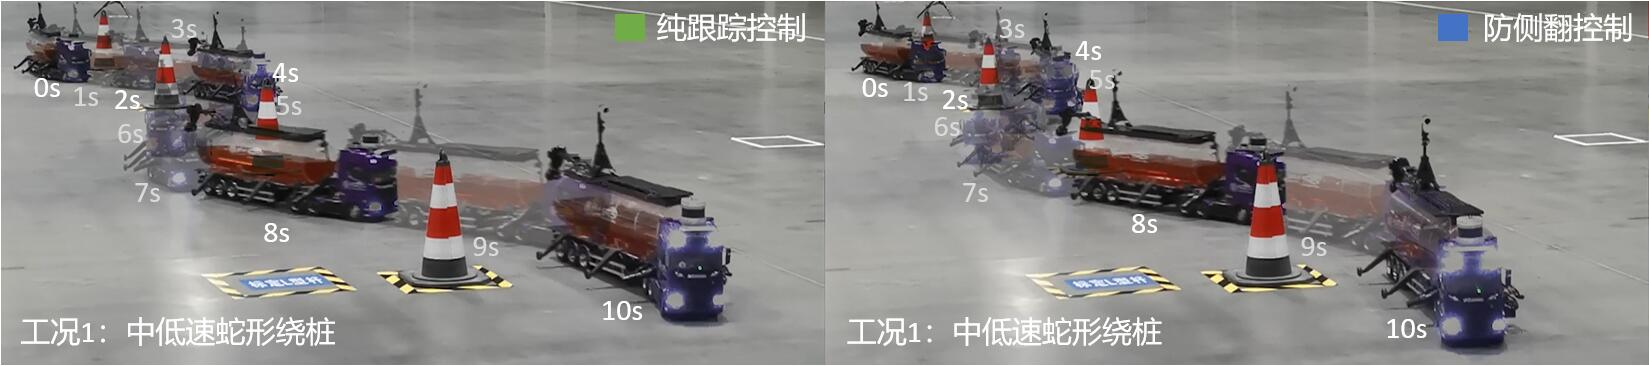
\includegraphics[width=1.0\linewidth]{fig/chap4/cond1_pic.jpg}}
        \subcaptionbox{工况2高速短距双移线实拍情况 \label{fig:cond2_pic}}
            {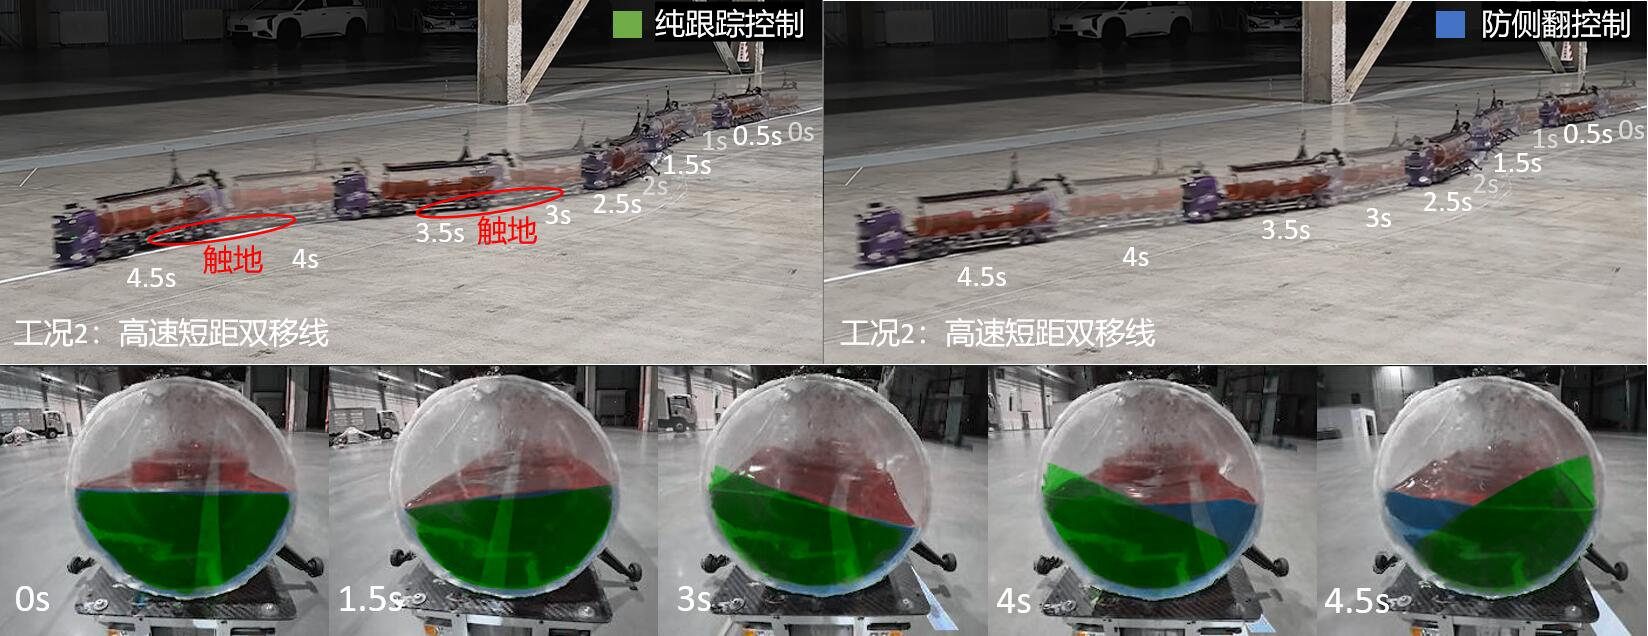
\includegraphics[width=1.0\linewidth]{fig/chap4/cond2_pic.jpg}}
        \caption{模型车试验实拍情况}
        \label{fig:cond_pic}
        \end{figure}


        两组实验中，车辆在蛇形绕桩时的中低速误差均保持在较小水平，维持了较高跟踪精度；在中高速稳态回转时，防侧翻控制由于采用多点跟踪方法，实现了更高跟踪精度。两种方法车速在全程基本保持一致，在双移线时均保持约\SI{2.5}{m/s}的行驶速度。

        如图~\ref{fig:exp_traj}所示，防侧翻组延迟驶回原车道，将LTR控制在软约束范围内，在避免侧翻事故发生的前提下尽可能保证了路径跟踪效果。防侧翻组将挂车侧倾角控制在\SI{\pm 5}{\degree}以内，液面最大倾角约为\SI{15}{\degree}；而纯跟踪控制组仅关注路径跟踪，虽跟踪误差较小，但过大的横向加速度引发了剧烈的液体晃动。图~\ref{fig:cond2_pic}显示，纯跟踪控制组的防侧翻支架分别在工况相对时间\SIrange{3}{3.5}{s}和\SIrange{4}{4.5}{s}触地。尽管防侧翻支架避免了实际侧翻事故，但该现象在实车场景下等同于侧翻事故。

        纯跟踪控制组在第一次变道结束时和第二次变道结束时，挂车侧倾角分别达到约\SI{6}{\degree}和\SI{7}{\degree}，相比之下防侧翻组的侧倾角最大降低了\SI{42}{\percent}。纯跟踪控制组的LTR在工况相对时间\SI{3}{s}和\SI{4.5}{s}时达到1，表明此时已存在侧翻风险。纯跟踪控制组出现了剧烈且显著非线性的液体晃动，其液面倾角多次达到\SI{20}{\degree}以上；而防侧翻组始终将晃动角度控制在\SIrange{-15}{15}{\degree}范围内，剧烈的液体晃动是引发侧翻的主要原因之一。

        \begin{figure}
        \centering
        \includegraphics[width=1.0\linewidth]{fig/chap4/exp_traj.jpg}
        \caption{模型车试验轨迹跟踪情况}
        \label{fig:exp_traj}
        \end{figure}

        \begin{figure}
        \centering
        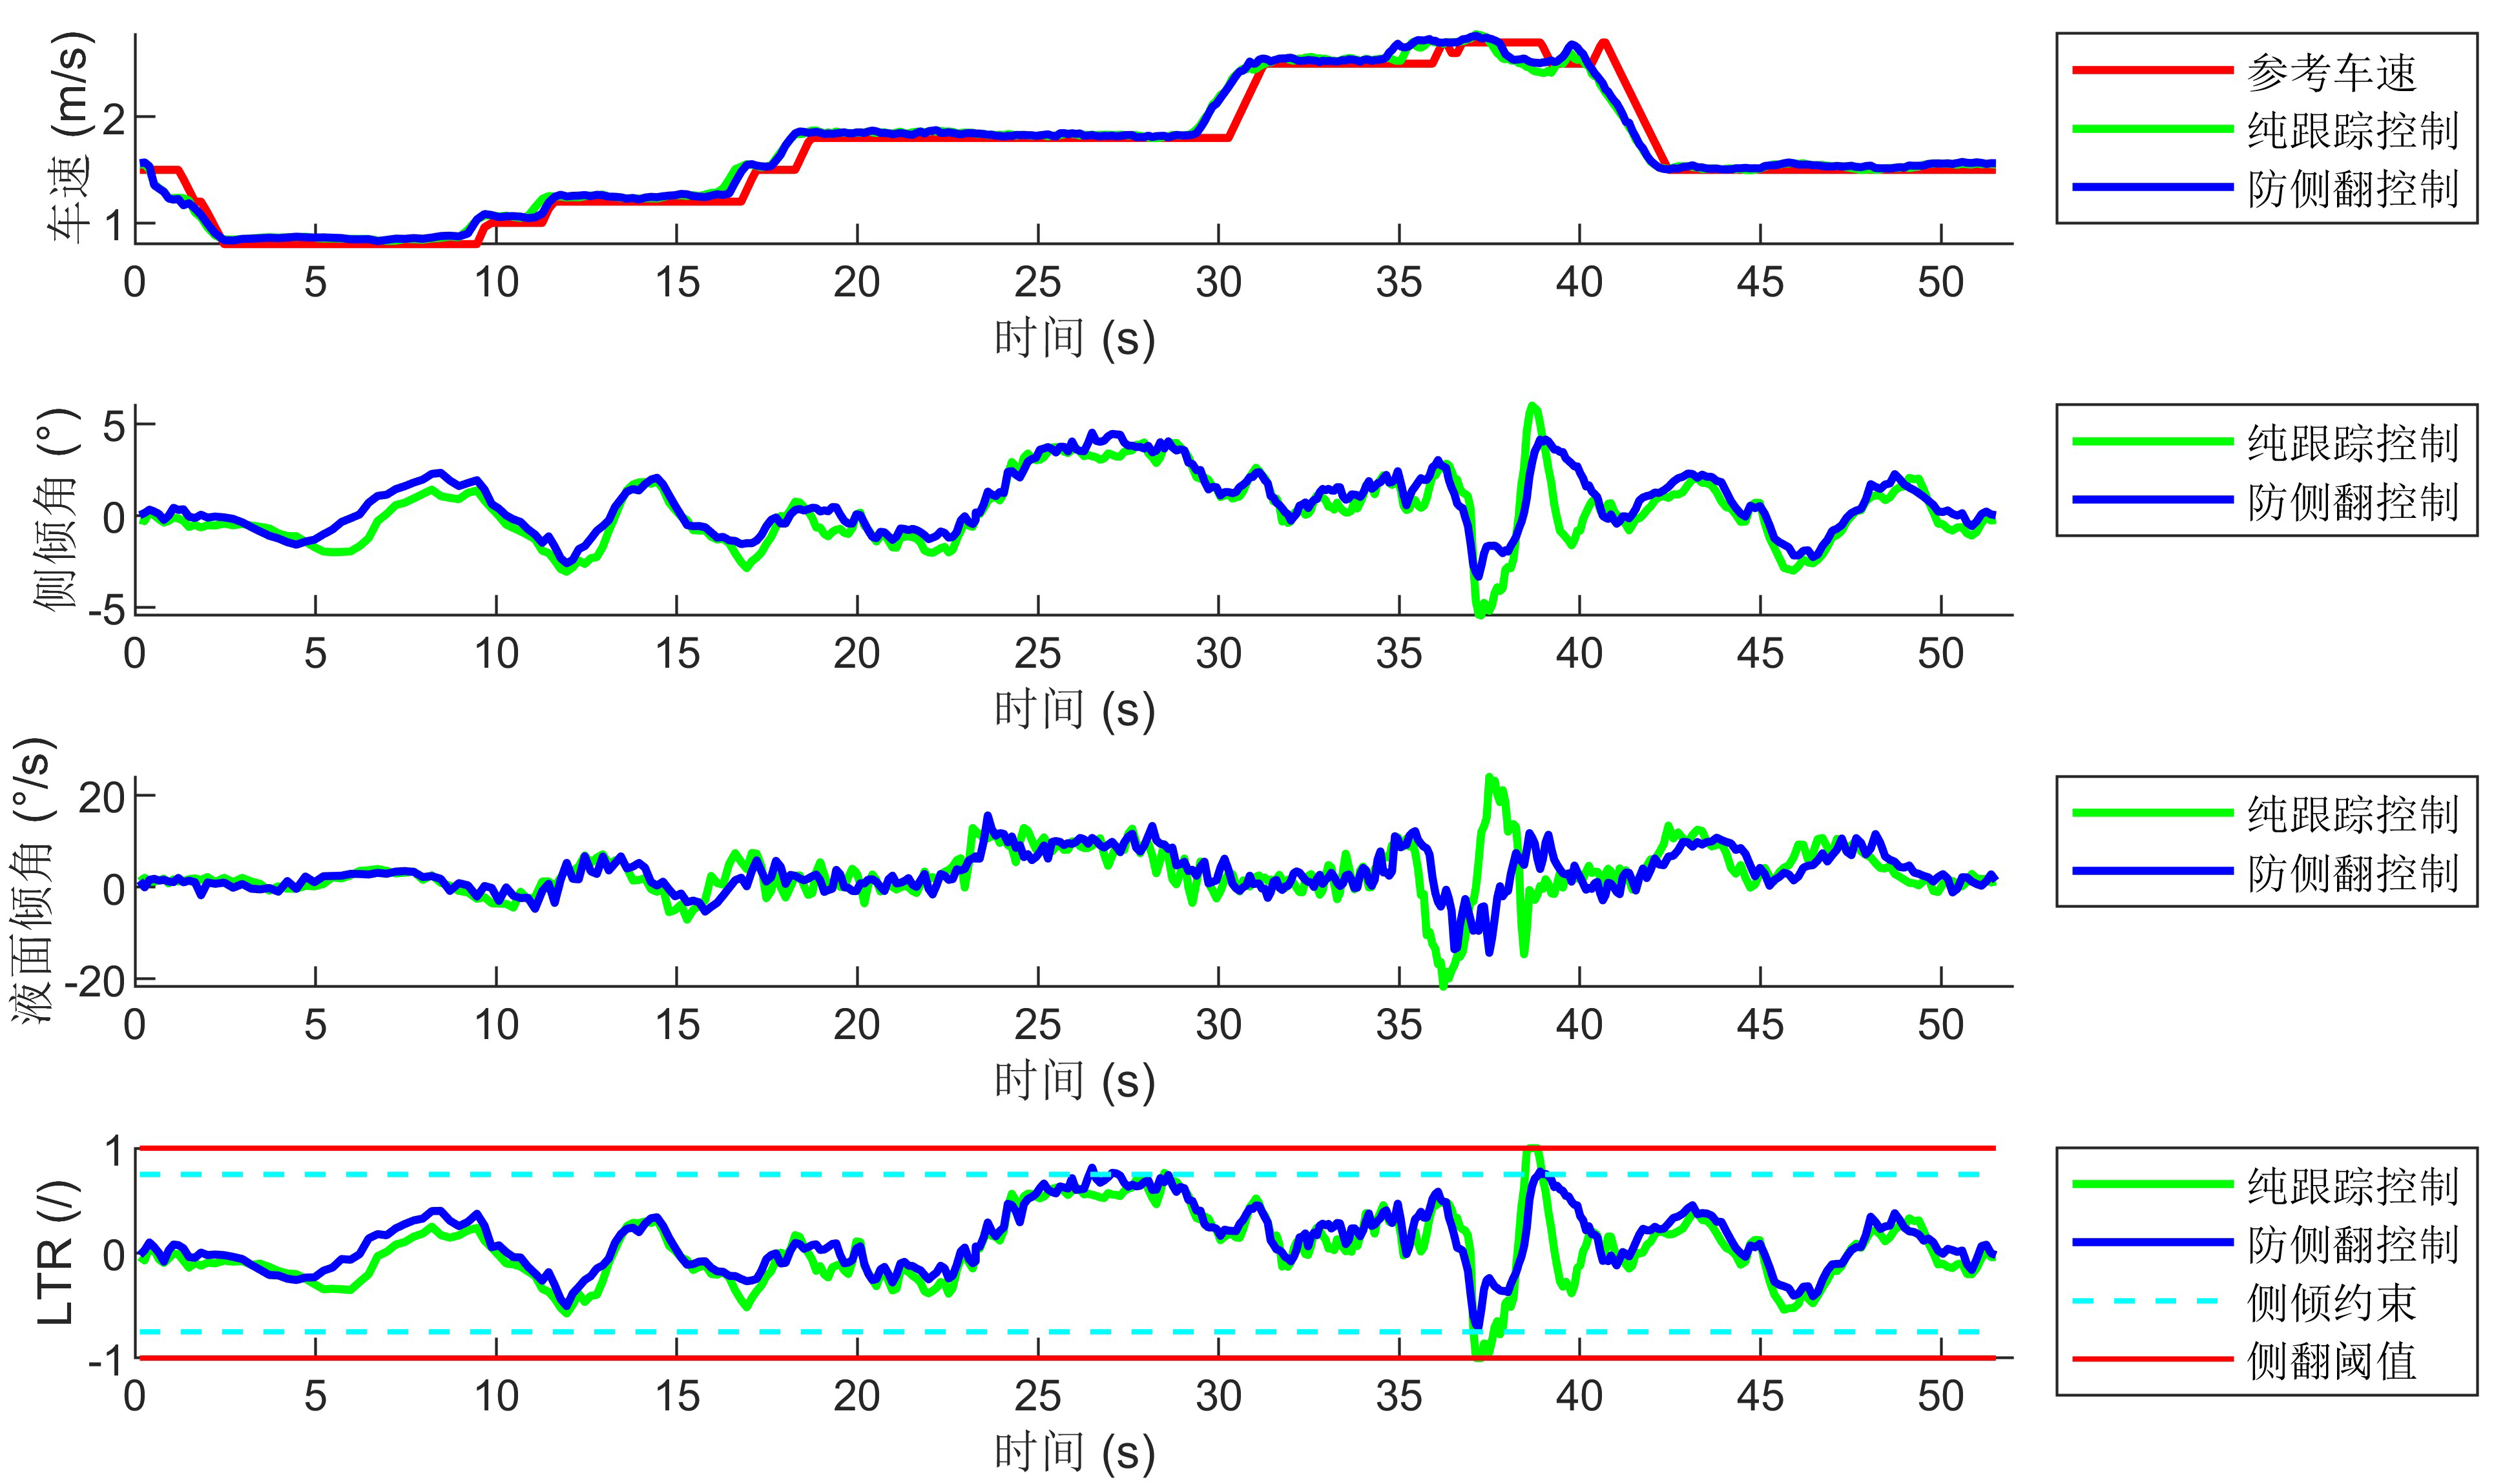
\includegraphics[width=1.0\linewidth]{fig/chap4/exp_x.jpg}
        \caption{模型车试验车辆状态量变化}
        \label{fig:exp_x}
        \end{figure}

        车辆控制量变化如图~\ref{fig:exp_u}所示，可以看出横向控制方面，防侧翻控制组倾向于输出更平缓的转角以抑制液体晃动并减小LTR峰值。求解器时间平均在\SI{15.4}{ms}，峰值求解时间小于\SI{25}{ms}，满足工程应用的实时性条件。

        \begin{figure}
        \centering
        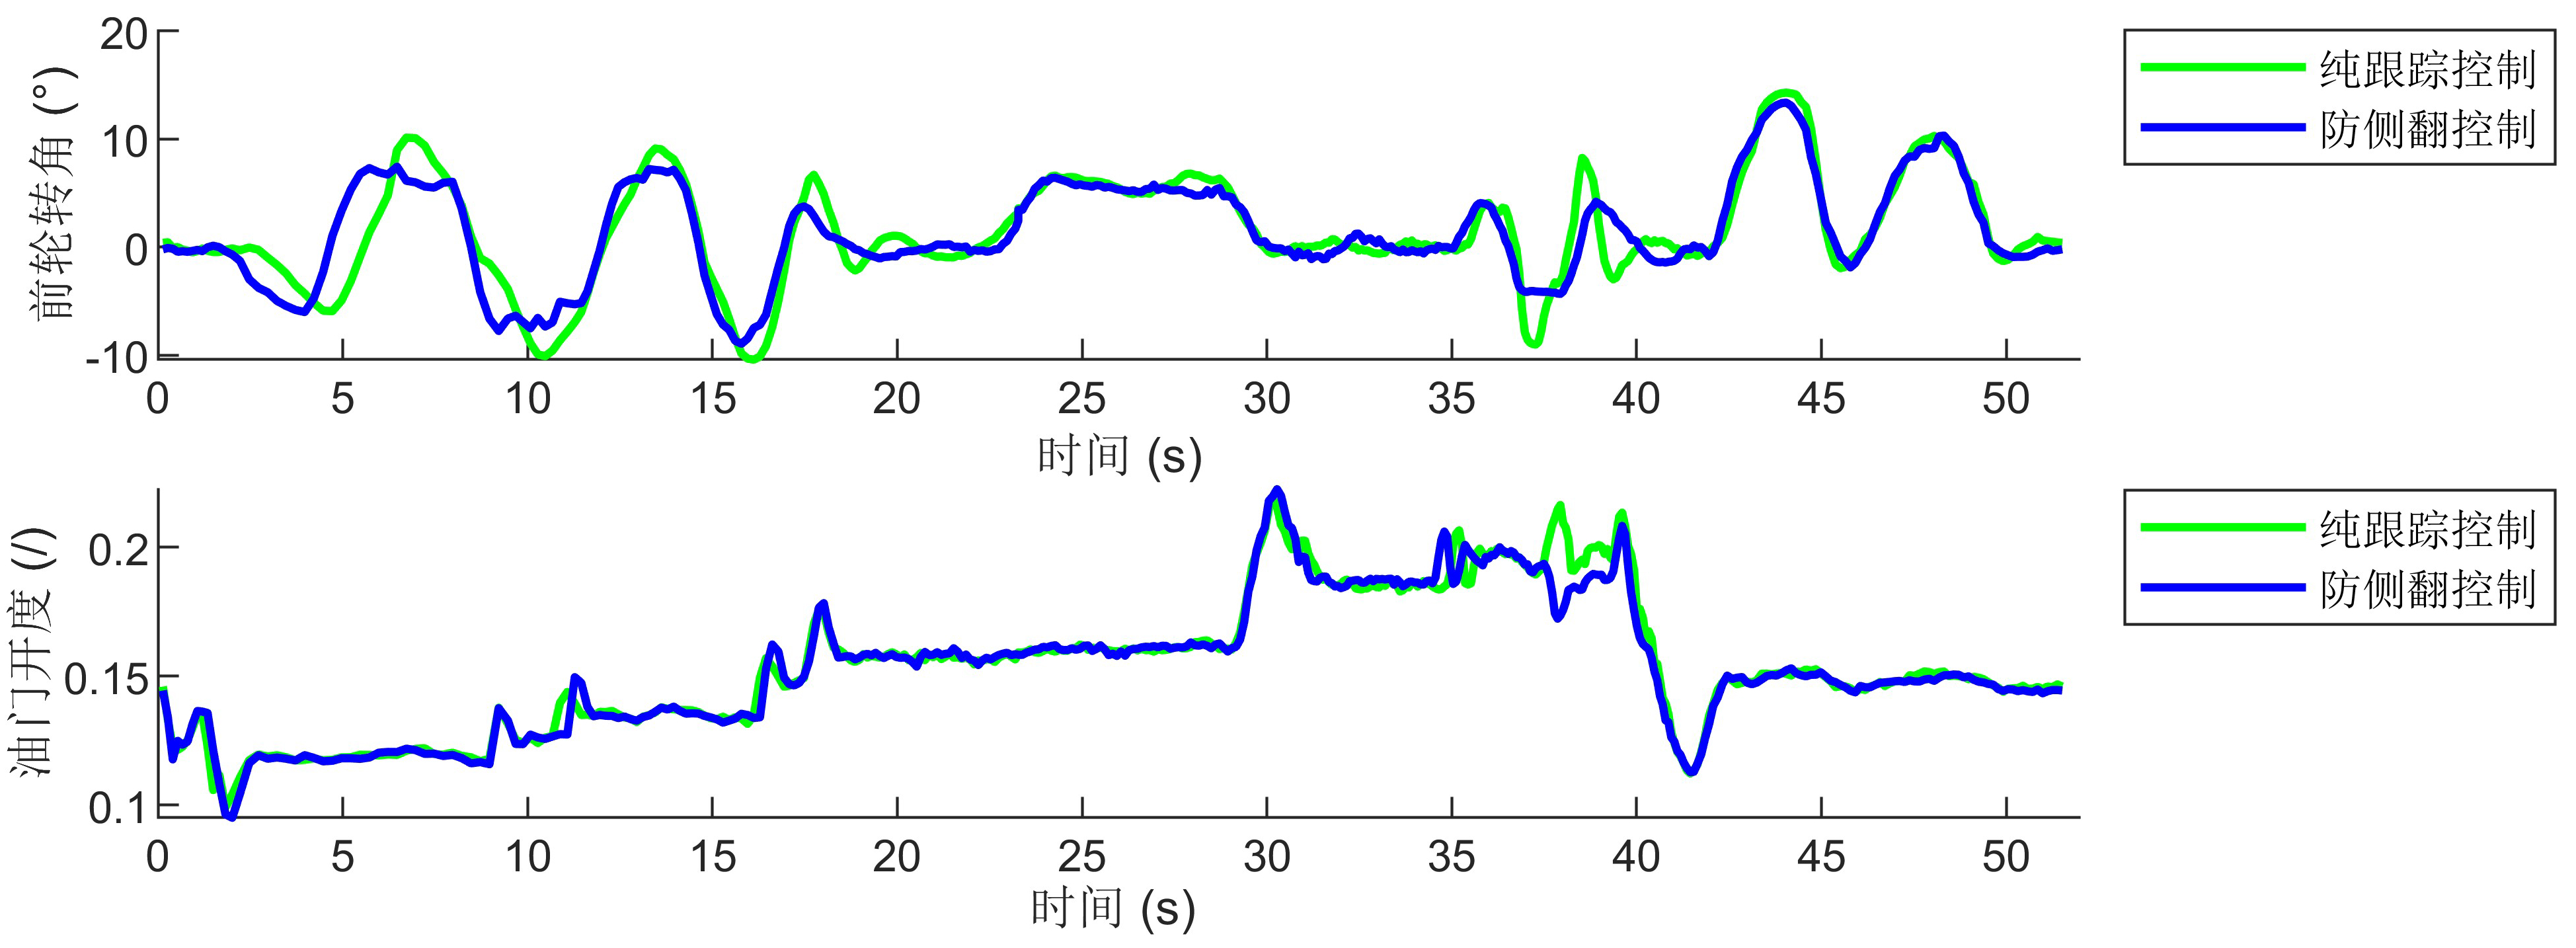
\includegraphics[width=1.0\linewidth]{fig/chap4/exp_u.jpg}
        \caption{模型车试验车辆控制量变化}
        \label{fig:exp_u}
        \end{figure}

        \begin{figure}
        \centering
        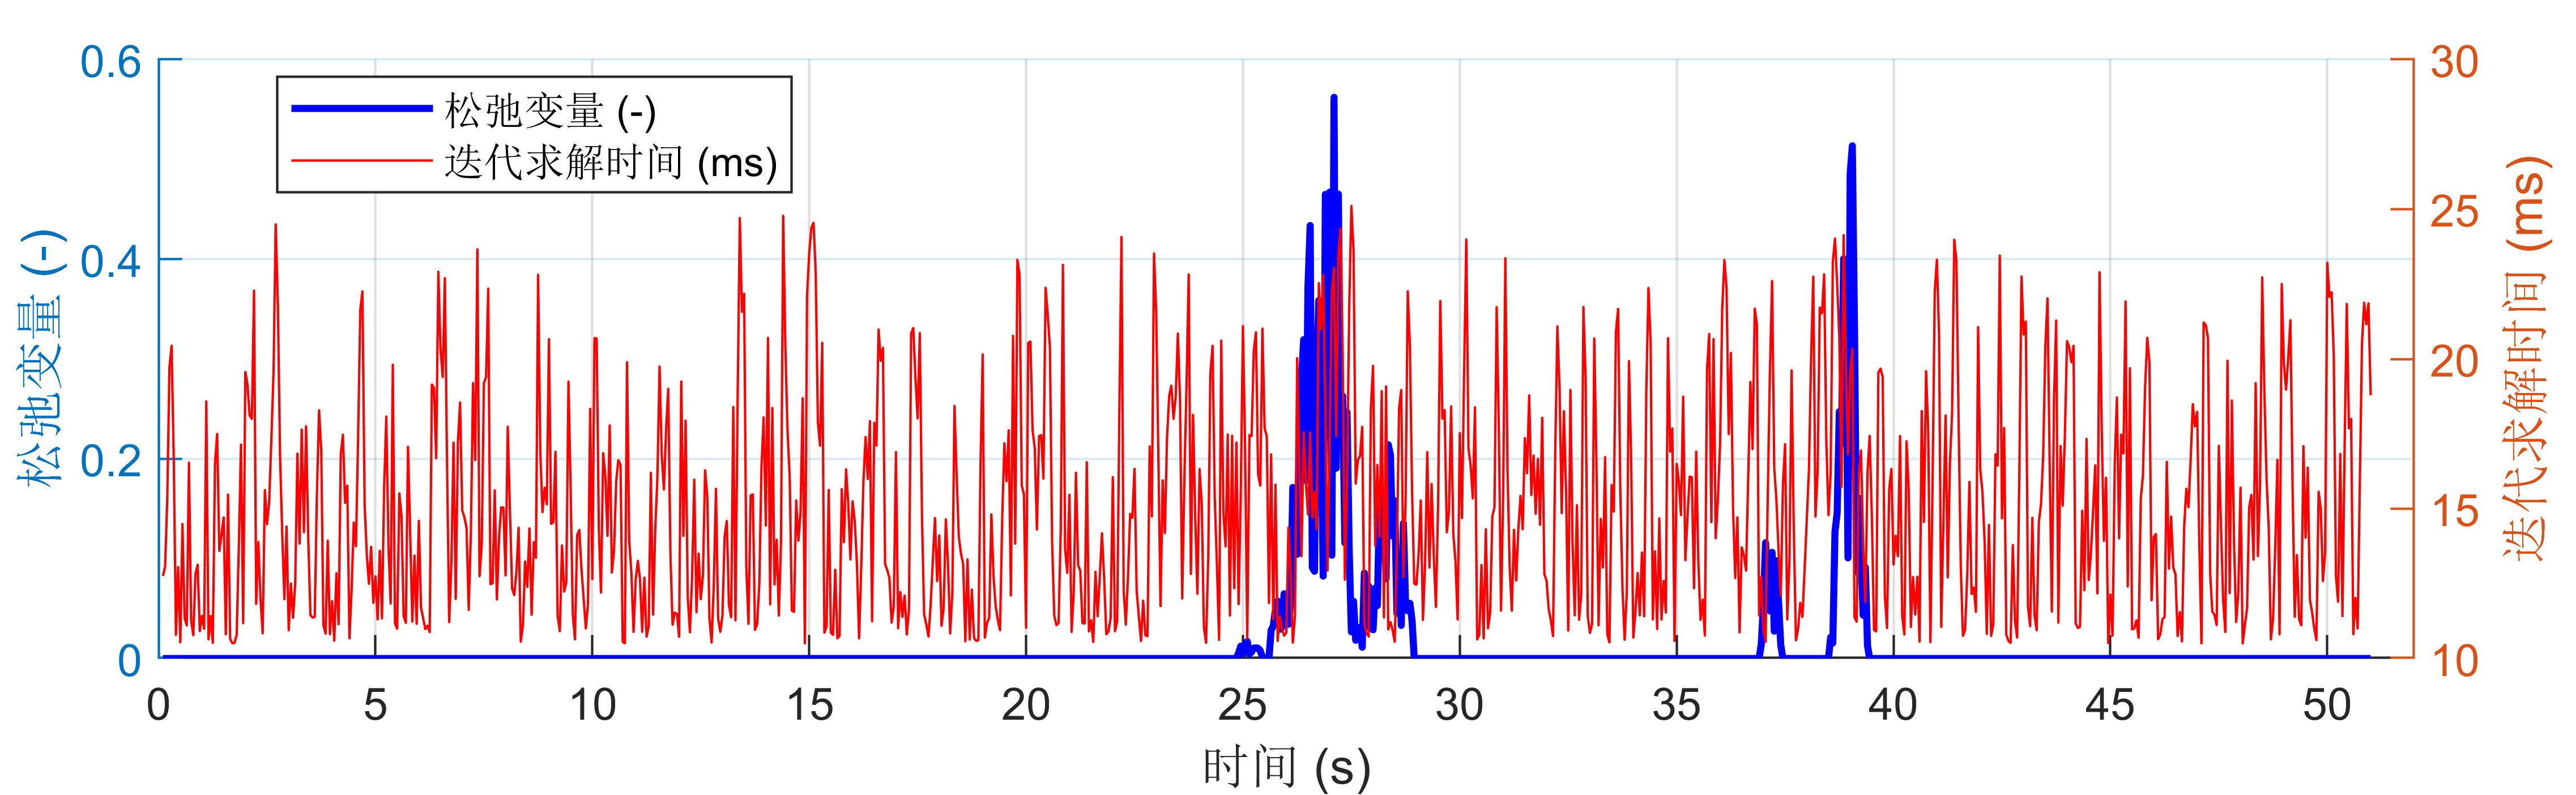
\includegraphics[width=1.0\linewidth]{fig/chap4/slack_iter.jpg}
        \caption{模型车试验求解时间与松弛变量变化}
        \label{fig:slack_iter}
        \end{figure}




\section{本章总结}
本章围绕车端稳定性干预，针对突发工况下液罐车侧翻风险的快速演化特性，构建了从车液耦合建模、在线可解防侧翻轨迹跟踪控制，到联合仿真与缩比模型试验验证的完整闭环，形成可支撑工程实时部署的车端防侧翻控制方案。主要工作总结如下：

\begin{enumerate}[label=(\arabic*)]
  \item 提出横纵向耦合液体晃动的滑动伸缩天平建模方法，并完成参数辨识与多工况验证。通过机械等效建模在力/力矩六自由度输出层面逼近高精度流体仿真结果，既刻画横纵耦合晃动，也能反映横摆及舱室液体转移的稳态变化，且计算效率显著优于高保真仿真，为在线控制提供高精度快速预测模型基础。
  
  \item 针对STL模型非解析、难以直接用于在线优化的问题，构建“基础解析模型+可学习残差”的重线性化框架。以线性双摆模型为解析基础，通过残差强化学习补偿模型误差并实现工况自适应，使复杂车液耦合动力学可在线求解，平衡精度与实时性。
  
  \item 建立横纵向耦合半挂液罐车动力学与多约束模型预测控制框架，实现抑晃防侧翻轨迹跟踪。将侧翻风险指标、轨迹跟踪误差、执行器约束及车辆动力学约束纳入优化问题，形成控制周期内可实时求解的稳定性干预策略；引入无模型自适应滑模残差补偿与差动制动，提升极限工况下的鲁棒性与稳定裕度。
  
  \item 搭建车液耦合联合仿真平台并完成多场景验证，结合缩比模型试验实证检验。左转弯、高速单移线等典型高风险工况中，所提方法可有效抑制侧倾与液体晃动、降低侧翻风险；缩比试验显示，防侧翻组侧倾角峰值最大降低约\SI{42}{\percent}，在线求解平均约\SI{15.4}{ms}、峰值小于\SI{25}{ms}，验证了工程可行性。
\end{enumerate}

综上，本章从高精度快速车液耦合建模出发，针对在线控制需求提出重线性化与残差补偿机制，多源验证证实了车端抑晃防侧翻轨迹跟踪控制的有效性与实时性，为下一步与云端预测性决策的协同闭环集成奠定车端基础。
